%!TEX TS-program = xelatex
%!TEX encoding = UTF-8 Unicode

\documentclass[School=EMC]{Dissertate}
\usepackage{tikz}
\usepackage{chapterbib}
\usepackage{natbib}

\usepackage{setspace}

\usepackage{pdfpages} % to include existing papers



%\newcommand\bookepigraph[4]{
%\vspace{1em}\hfill{}\begin{minipage}{#1}{\begin{spacing}{0.9}
%\small\noindent\textit{#2}\end{spacing}
%\vspace{1em}
%\hfill{}{#3}\\

%\vspace{-1em}\begin{flushright}{#4}\end{flushright}}\vspace{2em}
%\end{minipage}}


\newcommand\epigraph[3]{
    \vspace{1em}\begin{center}
    \begin{minipage}{#1}{
        \begin{spacing}{1.2}
        \small\noindent\textit{#2}\end{spacing}
        \vspace{1em}
        \hfill{}\small{#3}
    }
    \vspace{2em}
    \end{minipage}
    \end{center}
}


%\newcommand\anonymousepigraph[2]{
%\vspace{1em}\hfill{}\begin{minipage}{#1}{\begin{spacing}{0.9}
%\small\noindent\textit{#2}\end{spacing}}
%\vspace{1em}
%\end{minipage}}

\begin{document}

% the front matter
\begin{titlepage}
%\usepackage{tikz}
\tikz[remember picture,overlay]
\node[opacity=0.8,inner sep=0pt] at (current page.center){
    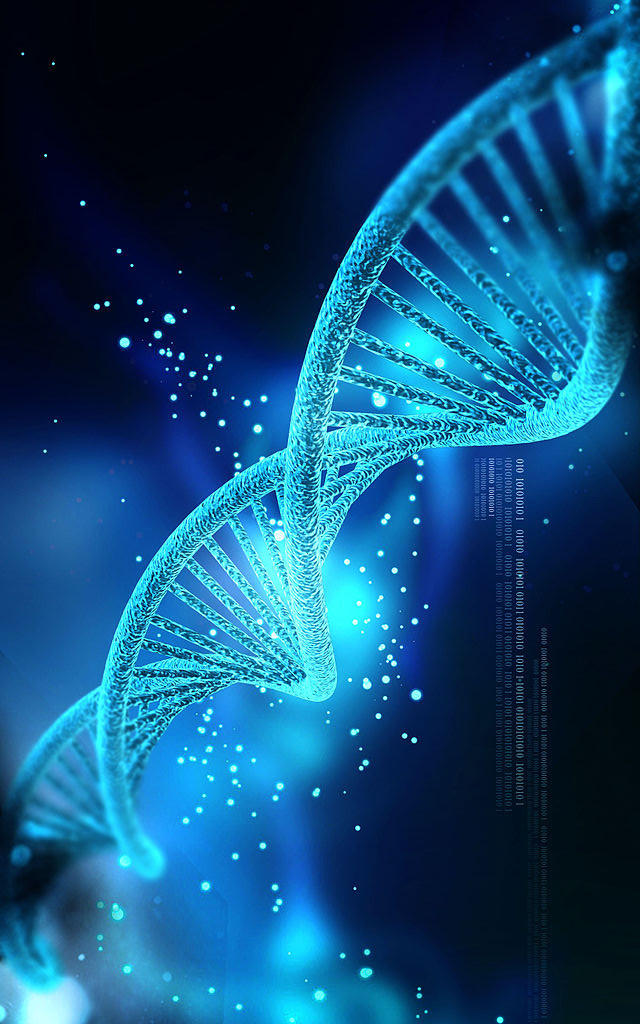
\includegraphics[width=\paperwidth,height=\paperheight]{frontmatter/images/cover2.jpg}
};
%\clearpage

\begin{center}

\color{white}{
\vspace{-2cm}
\huge{
    \sc{
    \textbf{ \uppercase{The Big Red Button}}} \\
    \normalsize toward the biologist's dream of a mystical button converting raw data into Nature papers

    \vspace{16.6cm}

    \LARGE Saskia Hiltemann}
}
\end{center}
\end{titlepage}

% Some details about the dissertation.
%\cleartorightpage
\title{Jigsaw Genomics}
\subtitle{Assembling the pieces toward open and accessible bioinformatics for all}
\titledutch{Jigsaw Genomics}
\subtitledutch{De puzzelstukjes op hun plaats leggen voor open en toegankelijke bioinformatica voor iedereen}
\author{Saskia Hiltemann}
\advisor{Bigname Scientist}
\rector{Prof.dr. R.C.M.E. Engels}
\defensedate{XX YY 2020}
\defensetime{00:00 uur}
\placeofbirth{Tilburg, Nederland}

% ... about the degree.
\degree{Doctor of Philosophy}
\field{Bioinformatics}
\degreeyear{2024}
\degreemonth{May}
\department{Bioinformatics}

% ... about the candidate's previous degrees.
\pdOneName{B.S.}
\pdOneSchool{Boston University}
\pdOneYear{2018}

\pdTwoName{M.A.}
\pdTwoSchool{Monster's Univeristy}
\pdTwoYear{2021}

\maketitle
\copyrightpage
%\abstractpage
\dedicationpage

% the abstract
\chapter*{Foreword}
\setlength\parindent{0pt}
\vspace{-1cm}
I like puzzles. Any type of puzzle. I always have. If I see a puzzle or a problem I have
to solve it. I think that is what makes cancer such a fascinating topic for me.

Imagine you are given a jigsaw puzzle. Now instead of a few hundred pieces, there are
several billion pieces. The picture on the box is not a picture of the puzzle inside the box,
it is just a somewhat similar image. Oh, and did I mention there are a whole bunch
of pieces missing? and that many pieces are duplicated? Some pieces don't even belong in our box,
but come from a completely different puzzle. On top of that your little sister has spilled paint
over some of the pieces so those can't be trusted to contribute to the image. And instead of one
single puzzle, the box contains several, they are all variations of the image on the box, but you have
no idea how many different puzzles the box contains.

Sound challenging? This is the problem we are solving whenever we sequence a cancer genome.

\vspace*{0.5cm}
\textbf{[Metaphor key]} \\
\textit{puzzle pieces} = sequence reads \\
\textit{picture on box} = reference genome \\
\textit{missing pieces} = hard-to-sequence areas \\
\textit{other puzzles} = contamination \\
\textit{painted pieces} = sequencing errors \\
\textit{multiple puzzles in box} = clonality

\verb+<thought: have the metaphor low-key run throughout thesis? >+

\chapter*{Stellingen}

(TODO: remove, just a placeholder for notes and ideas)


Eleven propositions must be added to the doctoral dissertation. Of these propositions,
five must relate to the contents of the doctoral dissertation and five must not relate,
either directly or indirectly, to the contents of the doctoral dissertation. These ten
propositions must be academically defensible. The eleventh proposition does not have
to meet the criterion of academic defensibility. The doctoral candidate must submit the
propositions to the doctoral dissertation supervisor as soon as possible following the
approval of the doctoral dissertation as referred to in Article 5.1.

\begin{itemize}
\item 5 from thesis, academically defensible
\item 5 unrelated to thesis, academically defensible
\item 1 anything goes, academically defensible or not
\end{itemize}

\begin{comment}
ideas

\begin{itemize}
\item This manuscript
    \begin{itemize}
    \item Training is pivotal

    \end{itemize}
\item Academia
    \begin{itemize}
     \item Scientists should write up results for general public as well as scientific journals
     \item Open science FTW, no more paywalled journals. or use money to pay peer reviewers to do thorough testing. or professional reviewers.
     \item Do we even need journals? system of completely open peer review could replace
     \item post-publication public peer review FTW
    \end{itemize}
\end{itemize}
\end{comment}

\chapter*{Scope of Thesis}

Chapter 1: General technical papers useful for many studies: Galaxy, iReport, Circos? \\
Chapter 2: Training Materials \\
Chapters 3-5: Technical paper \& the biological insight it led to/facilitated \\

\begin{enumerate}
    \item Tools: Galaxy, iReport, Circos(?)
    \item Training Materials
    \item Cancer - Fusion Gene detection: iFUSE \& VCaP Chromothripsis
    \item Cancer - Somatic Variant detection: CGtag \& Virtual Normal
    \item Microbiota profiling: GmT \& MYcrobiota
\end{enumerate}


\tableofcontents
%\authorlist
%\listoffigures

\abstractpage
%\doublespacing

% include each chapter...
\setcounter{chapter}{-1}  % start chapter numbering at 0 because (computer) science
\chapter{Introduction}
\label{introduction}
 % start numberings at 0 because (computer) science
\setcounter{figure}{-1}
\setcounter{table}{-1}
\setcounter{section}{-1}
\setcounter{NAT@ctr}{-1}

\setlength\parindent{0pt}


\begin{comment}
\section*{Contents}
\begin{enumerate}
\itemsep-0.5em
\item A Brief History of Genomics
\item A Primer on Sequencing (?)
\item The Bioinformatics Challenge
\item Bioinformatics Best Practices
\item The Galaxy Platform
\item Use case 1: Prostate Cancer
\item Use case 2: Microbiota Analysis
\item Scope of this Thesis.
\end{enumerate}
\end{comment}


\section{The Source Code of Life}

DNA. The blueprint of life. These long double-stranded helical molecules are present in all living cells on earth\footnote{As far as currently known. Some viruses contain only RNA, but these are often not considered "alive".} and encode the proteins which drive the functioning, regulation, structure and replication of the cells and tissues that make up an organism. In many ways, DNA is also analogous to computer code; any computer program, no matter how complex, can be described as a long series of just two characters, \verb+0+ and \verb+1+, known as \emph{bits}. Knowing the sequence of these bits and, crucially, the details about how they are being interpreted by the machine on which they are executed, lets us understand and predict the functions they encode. In much the same way, DNA uses just 4 different elements, called \emph{bases} or \emph{nucleotides}, to encode its blueprint for the cell. These 4 building blocks are adenine, cytosine, guanine and thymine, usually referred to simply by their first letters, \verb+A+, \verb+C+, \verb+T+ and \verb+G+. These bases combine together in pairs (\emph{base pairs}), with \verb+A+ always matching to \verb+T+ and \verb+C+ being complementary to \verb+G+ along a sugar phosphate backbone in their double-helix configuration (Figure \ref{fig:dnastructure}).

\begin{wrapfigure}{r}{210pt}
%\begin{figure}[h!]
    \centering
    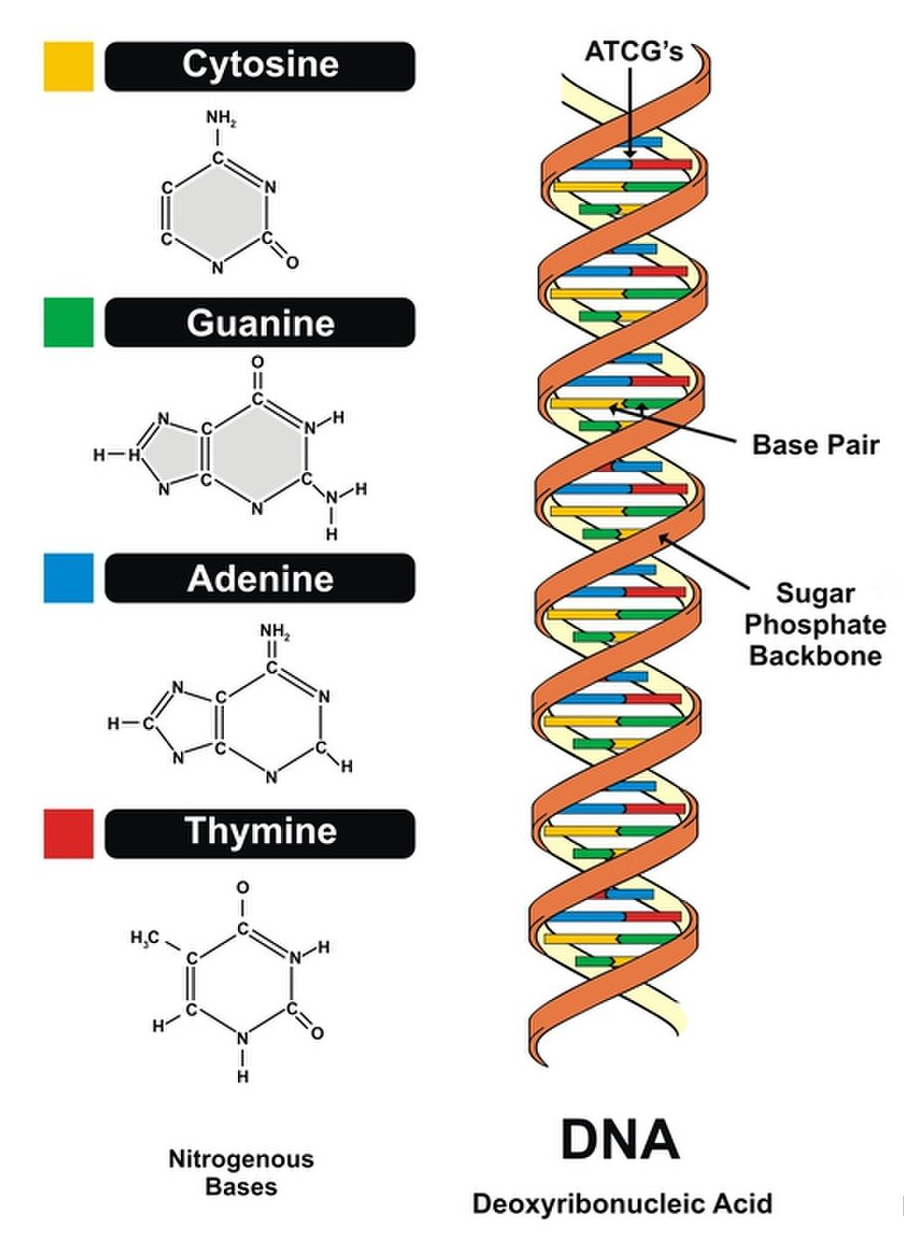
\includegraphics[width=200pt]{chapters/images/introduction/dna-structure.png}
    \caption{Structure of DNA}
    \label{fig:dnastructure}
%\end{figure}
\end{wrapfigure}

In humans, DNA is organised into 23 pairs of chromosomes, with a total length of over 3 billion base pairs. About 1\% of this DNA make up \emph{genes}; stretches of DNA which directly encode protein molecules. When these genes are expressed, the gene sequence is transcribed to a messenger molecule (\emph{mRNA}) which is subsequently translated into a protein molecule. The function of the remaining 99\% of the genome long remained a mystery, and was even referred to as \emph{junk DNA}. More recent studies have revealed that these stretches of non-coding DNA play an important role in the regulation of the expression of genes, stimulating or prohibiting the translation of genes to proteins and thereby influencing the functioning of the cell. For any two individuals, the vast majority of their DNA sequence will be identical, but small variations in the remaining locations of the genome are what make each of us unique. But it is also what can make us sick. Studying this natural variation in the genome sequence helps us unravel the mechanisms of life and disease.


\subsection{A Brief History of Genome Sequencing}
Friedrich Miescher was the first to isolate DNA molecules (which he termed \emph{nuclein}) in 1869. However, the molecule remained relatively understudied until Rosalind Franklin used X-ray crystallography to inspect the molecule's structure \cite{elkin2003rosalind}. Watson and Crick famously used this data to postulate the double-helix model of DNA in 1953 \cite{watson1953molecular}. This model illustrated for the first time that DNA molecules we ideally suited for replication, and solidified the idea that DNA, and not protein as was previously thought, was the primary carrier of hereditary information. Simultaneously, Frederick Sanger had developed techniques to sequence proteins, and later RNA and DNA molecules. This was the start of first generation of genome sequencing, and the first full gene was sequenced in 1972 () \cite{TODO}, followed by the first full genome in 1976 (bacteriophage Phi X 174, 5386 nucleotides long) \cite{}. These early techniques were only suitable for relatively small sections of DNA, and more technological advances would be required before larger genomes could be fully sequenced.

In 1990, the Human Genome Project \cite{olson1993human} set out to sequence the entire 3.2-billion-basepair-long human genome, an effort culminating in 2003 with the publication of the first human \textit{reference genome} \cite{international2004finishing}. Not only did this provide invaluable insights into human genetics, but it also paved the way for the next era in genetic research; something which would completely transform the field of genetic research. Over the next several years, next-generation massively parallel sequencers were developed by companies like Roche454 and Illumina, dramatically cutting the cost and time required to sequence a human genome, and for the first time demonstrated its potential utility in clinical and diagnostic settings. Through sustained technological advancements over the following years, these costs continued to decrease at exponential rates - outstripping even the pace predicted by Moore's law (\hyperref[fig:seqcost]{Fig. \ref{fig:seqcost}}) - and the long dreamed-about \textit{\$1,000 dollar genome} \cite{thousanddollargenome} \cite{sequencingcostsNHGRI} has now become a reality.

\begin{figure}[h!]
    \centering
    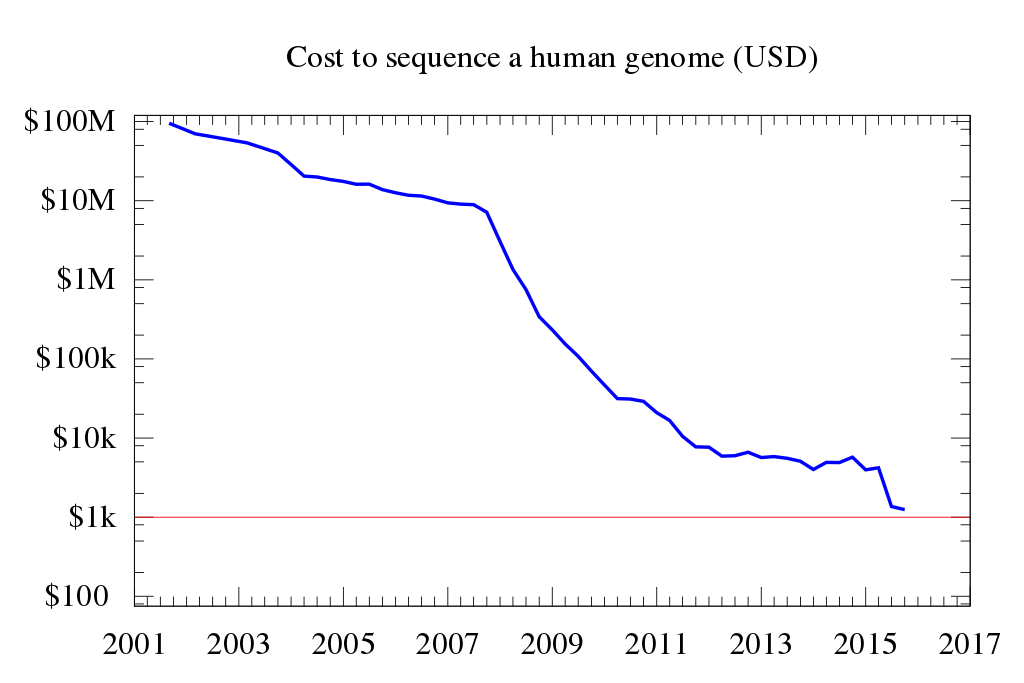
\includegraphics[width=300pt]{chapters/images/Historic_cost_of_sequencing_a_human_genome.png}
    \caption{The cost of sequencing a human-sized genome over time. Data from the NHGRI Genome Sequencing Program (GSP) }
    \label{fig:seqcost}
\end{figure}

Shortly after the publication of the human genome, high-throughput techniques emerged to also sequence the transcriptome (RNA-Seq), allowing for the identification and quantification of gene transcripts, and providing information about post-transcriptional mutations and other complexities such as alternative splicing \cite{wang2009rna}. Similarly, the study of epigenetics is revealing that non-coding DNA, far from the once-termed \textit{"junk DNA"}, is part of an intricate and complex regulatory system controlling the expression of genes \cite{zuckerkandl2007combinatorial}.

Now we are now moving into the era of third-generation sequencing, where single-cell \cite{gawad2016single}, long-read \cite{koren2015one}, and often real-time sequencing \cite{flusberg2010direct} are allowing for ever more accurate determination of nucleotide sequence, providing increased resolution even in highly diverse and complex samples such as cancer or metagenomic samples. All these technological advances have led to a deluge of data that must be managed and analysed, typically by bioinformaticians.


\section{The Bioinformatics Challenge}

With huge amounts of data now being generated at relatively low cost \cite{chen2014big}, and compute resources being available even on moderate budgets, the challenge in genomic research has shifted from the sequencing technologies to the analysis and interpretation of these big and highly complex datasets, and the development of the software required to do so, in order to gain new understanding of the underlying biological systems. This poses a significant challenge, both technologically and scientifically.

\subsection{Ever-changing landscape}
Sequencing technologies are evolving at a staggering pace, and with them, so must the software tools capable of analysing the data. Therefore, new tools are developed continually and existing tools must be updated regularly to remain relevant. As a consequence, there typically simply is not enough time for community standards and consensus analysis pipelines to emerge organically before the advent of new technologies make them obsolete. Because of this, there usually are a multitude of tools available for any given task, each with their own set of advantages and disadvantages, and the challenge is to find the right tool for the particular situation, and knowing when to use existing tools and when the development of novel tools is in order.

\subsection{Standardisation}
Such a lack of clear standards does not only apply to software tools, but also to file formats, and this poses a major hurdle in data analysis. While some clear data format standards exist [fastq, VCF], there are many cases that lack such a standard, hindering the interoperability of different tools. And even the more established file formats such as fastq and VCF allow for a variety of flavours, e.g. different fastq quality encoding schemes, which are not indicated inside the file format specification itself, but may influence downstream results. Thus, when creating analysis pipelines from existing tools, many file transformation steps are typically required as a kind of \textit{glue} between steps.

\subsection{Data Storage}
 \begin{comment} https://qumulo.com/blog/genomic-sequencing-qf2-storage/ \end{comment}
Sequencing data is being generate at a rate of X petabytes per year (TODO: find citation), and all this data must be stored somewhere. But there is more to data storage than buying a hard disk and copying data. The data must be backed up to prevent data loss, it must be made available for use in an efficient way (I/O matters), data must be organised and tracked in a usable manner, and any solution must be able to scale to the exponential trend of growth both in size and number of files generated. Furthermore, data storage must comply with privacy and security requirements, especially important in the case of human genetic data.


\subsection{The Specialist Bioinformatician}
All of these challenges have resulted in bioinformatics becoming a highly specialized field, which in itself poses a new challenge given the observation that the domain knowledge (biology) and the informatics know-how more and more often do not reside in a single individual, and the interpretation of the data cannot always be done by the person performing the data analysis and vice versa. Instead, close communication between the two fields is required, and the domain experts should be empowered to perform their own data analyses as much as possible.

\verb+informatician needs to shine a light in the black box that is the wetlab, domain expert needs to become comfortable with the informatics, since this has become an integral part of any analysis+


% some (partial) solutions to the above challenges, spoilers: open software, open science, open everything
\section{Bioinformatics Best Practices}
Since bioinformaticians are primarily academics -who are typically being judged on their publications, not their code-, the quality of bioinformatics tools is highly variable and tool authors often struggle to find the time and resources to maintain their code. The open-source community is instrumental in this respect, allowing the most popular and useful tools to be taken up by the community which can collectively maintain and update the bioinformatics software packages. Adhering to a set of best-practices guidelines can greatly reduce this maintenance burden, and increase the chance of tools being taken up by the community.

Many journals require authors to submit datasets to public repositories in order to allow other scientists to reproduce their findings. With bioinformatics now such a fundamental part of any publication, a clear description of the analysis pipeline is also required for true reproducibility, but the majority of scientific publication do not contain all the information required to reproduce the in-silico experiment [cite]. Making analysis software open-source and adhering to a set of bioinformatics best-practices can improve the reproducibility of bioinformatics analysis pipelines.

Such bioinformatics best-practices include:

\begin{enumerate}
    \itemsep-0.5em
    \item Accessibility of tools and data %(usability) of tools (documentation, open source, github etc, galaxy, galaxy, dependency management, docker)
    \item Reproducibility %(conda, docker, galaxy, version control, code notebooks)
    \item Interoperability %(data formats, common frameworks, generic, allow for packaging)
    \item Maintainability of software %(testing, continuous integration, community buildingi, scalability)
    \item Visualization and reporting
    %\item Data management and sharing %(FAIR data, LIMS, PIDs)
\end{enumerate}


\subsubsection{Accessibility}
Most bioinformatics tools are commandline unix tools, and biologists are not typically trained in the use of such. Even for the experienced bioinformatician, running some of these tools can be a challenge due to lack of documentation or quality of the tool. Ideally, once a tool or pipeline has been validated, the analysis can be run by the domain expert, i.e. the research scientist responsible for the interpretation of the analysis results, without being reliant on the support of a bioinformatician at every step \cite{kumar2007bioinformatics}.

Creating user-friendly software is not a trivial task. Application linking (also referred to as wrapping), can ease this burden for the tool developer. In such an approach, existing user-friendly interfaces host third-party software packages -at miniumum effort to the developer of the hosted software- and thereby offer a layer of abstraction to the end-user that shields them from the implementation details of the tool and provides a uniform usage paradigm for all tools, regardless of their differences behind the scenes. Examples of such hosting frameworks in the context of bioinformatics are Galaxy \cite{giardine2005galaxy,goecks2010galaxy}, Taverna \cite{}, [more?].

Accessibility also includes high-quality documentation of the tool, both for developers and end-users, and ideally some form of training manual to educate users in the proper use of tool and warn about possible pitfalls and biases.

\subsubsection{Reproducibility}

A cornerstone of the scientific method is reproducibility of results. Experiments should be described in sufficient detail to allow for their reproduction and independent verification by fellow scientists. In reality however, this remains a big challenge, and many publications can not be reliably reproduced based on the information provided in publication []. In many cases this holds not only for the wetlab experiment, but also for the in-silico downstream data analysis. Reproducing bioinformatics analyses often becomes an exercise in \textit{"forensic bioinformatics"}; trying to piece together the exact procedure used through trial and error and educated guessing. In part this is caused by journals not having clear submission guidelines for bioinformatics pipeline description as they do for the physical samples. The latter are commonly required to be submitted to biobanks before submission, and the raw datasets generated from them to be stored in online repositories. No such requirements are generally imposed on the downstream analysis, or when they are these requirements are not strict enough to ensure true reproducibility. This is not without consequences; in some cases this has lead to clinical trials being started based on incorrect conclusions not revealed during peer review due to lack of reproducibility \cite{baggerly2009reproducible}.

% dependency management
But even if the full source code were made available, reproducibility of the entire dependency chain of all software and system libraries used remains problematic. Every package in this dependency tree has the potential to influence the final result. While reproducibility is a high priority in the scientific community, this isn't the same for software developers in general, and many packages will simply be removed when an update has been made available. This is where package managers such as Conda \cite{gruning2017bioconda} or GNU Guix \cite{courtes2013functional} offer significant improvement, by allowing specific versions of tools to be installed, and mandating that any changes made to a package must be submitted as a new version, and existing version remain available and unchanged indefinitely. This ensures that the stack of software obtained when installing a tool at a specific version will yield identical results today as it will a year from now.

% provenance
Once the correct set of software is obtained, the provenance of how the tools were applied to the data must also be logged. This includes the sequence and interplay of different tool executions, with the full parameter settings and input and reference data used at every step. Keeping a lab journal of the in-silico experiment is a good start, but too error-prone as a manual process. Projects such as Jupyter Notebooks \cite{kluyver2016jupyter} for Python, or Sweave \cite{leisch2002sweave} and KnitR \cite{xie2014knitr} for R, allow for the mixing of text and tools to create interactive journal articles if you will, where the calculations are embedded within the manuscript, and these calculations can be examined and rerun or adjusted with ease. A drawback of this of course comes when tools require a lot of resources or are not all written in the same language, as is typically the case for NGS analyses. Workflow platforms such as Galaxy \cite{} automatically keep track of provenance for the user and have the advantage of supporting a wide range of tools.


\begin{comment}
"forensic bioinformatics" -> have to figure out by trial and error what was done

https://bmcmedresmethodol.biomedcentral.com/articles/10.1186/s12874-017-0377-6
https://www.biostars.org/p/52561/
https://www.nature.com/naturejobs/science/articles/10.1038/nj7396-137a
https://www.nature.com/nm/journal/v13/n11/full/nm1107-1276b.html
\end{comment}

\subsection{Interoperability}

A plethora of bioinformatics tools are available, and most analyses require combining a number of tools together into an analysis pipeline, also referred to as a workflow. The different components in such a pipeline usually do not work seamlessly together without a bit of "glue"; custom scripts that convert the output of one tool so that it can be used as input for the next. This is necessary due to the frequent lack of clear data formats. For example for structural variations, no clear data format exists, and most tools output custom formats. Many of these custom formats contain the same information, it is often formatted differently. Any tools working on such datasets make assumptions about its format, so we must take care to adhere to these expectations. Even in cases where file formats are more standardized, variations in the exact implementations may still require careful consideration within a pipeline. Consider for example the fastq format; this is a relatively simple format, just 4 lines per sequence read, but the fourth line, the line containing quality score, is the source of some divergence in the format. A range of ASCII characters is used to encode numerical values indicating a PHRED-like quality score of the base call, but the range and start position of this character range comes in different flavours. Furthermore, because these ranges overlap, it is not always possible to deduce which convention was used unless some quality encoding are present in the file that only appear in one of the conventions. It is therefore important to know the convention used for any datasets entering your pipeline, and know when tools make assumptions about their input data. If necessary, a format conversion step can be employed to resolve any mismatches between the format expected by a tool and the format of the input dataset. Similar widespread variations in standard formats include chromosomal location (0-based or 1-based numbering, open or closed) and chromosome names (with or without a `chr` prefix). These issues are not hard to deal with, but can lead to inaccurate results if not carefully taken into account by the creator of the pipeline.

% packaging
On a more technical level, different tools may be written in different programming languages and/or compiled for different operating systems, and it can be a challenge to combine these into a single analysis. Luckily, tool developers can undertake steps to make their tools more interoperable. Package managers such as bioconda will compile software from its source for different operating systems. For bash scripts, many OS-dependent syntax variations can hinder interoperabililty, but by taking care to comply with POSIX standards, such concerns can be mitigated. Vitally, precise documentation of any assumptions made in the code is indespensible, and making source code open further facilitates this transparancy.


\begin{comment}
file format standards, common frameworks, good documentation, open-source,
allow for packaging (don't deliver code as VMs etc),
\end{comment}

\subsection{Maintainability}
In bioinformatics, the emphasis for scientific accomplishments is placed on scientific publications, not on software products. As a result, many tool developers struggle to find the time and resources to maintain their software beyond its release. Since scientific research depends increasingly on these pieces of software, decreasing the burden of tool maintainence is valuable and worthwhile pursuit. Furthermore, many tools are written by small research groups or single individuals who are simply unable to perform the necessary maintainence without support. By making tools open-source, the entire bioinformatics community is able to step up as co-developer, allowing them to discover bugs and contribute fixes or enhancements. Code sharing platforms like GitHub \cite{} and BitBucket \cite{} facilitate this community-driven approach to software maintainance.

Using code versioning such frameworks such as git \cite{} or mercurial \cite{} ensures precise tracking of changes and ability to revert to any previous state at minimal effort, and facilitates merging of that Incorporating tests at every phase of development can further decrease the maintenance effort. Unit tests ensure that small code modules show expected behaviour at all times. Functional tests ensure that these different units of code always yield the desired result when working in conjunction. Code quality checks can help streamline the code itself and increase readability, benefiting future development. Continuous integration is the paradigm whereby changes to the mainline code are incorporated incrementally and continually, and thoroughly reviewed and tested at every stage.

%versioning continuous integration, functional testing, code review, dependency resolution (conda)

\subsection{Visualisation and Reporting}

As scientists become increasingly reliant on large and complex computational analyses in their research \cite{chen2014big}, the final analysis result datasets become similarly complex and have  often grown beyond the realm of what can be manually viewed and interpreted, both in terms of the number of files and their sizes, as in terms of complexity. Analysis results therefore require summation and visualisation and must be presented to the domain expert in a comprehensible and accesible manner. Such a report should also contain detailed descriptions of the methods used and assumptions made and citations to any third-party tools employed, as an understanding of these factor can assist in interpretation \cite{kumar2007bioinformatics}.

For genomics data, visualisation tools such as Circos \cite{circos} [list more examples] enable the integration of various output datasets, often in the order of millions of lines each, to be summarized in a single image. While some resolution may be lost in such visualisations, they do enable the easy identification of areas of interest and guide the interpretation by pointing the domain experts in the direction of further inspection.


\section{The Galaxy Project}
The Galaxy project \cite{afgan2016galaxy} facilitates many of the best-practice bioinformatics guidelines outlined in the previous section. Galaxy provides a graphical web-based interface to commandline bioinformatics tools, bringing the data analysis to the domain experts equipped to perform the interpretation of the results. With its heavy focus on accessibility and reproducibility, Galaxy is an important component in creating high-quality bioinformatics pipelines. Galaxy keeps track of the full analysis provenance, manages tool dependencies with bioconda \cite{}, has built-in visualisations, and is accesible by end users with nothing more than a browser. For developers, Galaxy provides a convenient framework to package tools to make these available for researches throughout the global community. The Galaxy toolshed

\section{Training}
With -omics research becoming increasingly computational in nature, and many research groups not having access to a dedicated bioinformatician, there is a great need for high-quality bioinformatics training to ensure that the domain experts who interpret the results of data analyses are optimally equipped to do so. Surveys confirm this need for bioinformatic training; the majority of researchers (>95\%) work with or plan to work with large datasets, but most (>65\%) possess only minimal bioinformatics skills and are not comfortable with statistical analyses \cite{larcombe2017elixir}, \cite{williams2017vision}. Demand for training currently greatly exceeds the supply \cite{attwood2017global}. In a recent survey \cite{survey2013embl} over 60\% of biologists expressed a need for more training while only 5\% called for more computing power. Thus one can assume that the true bottleneck of the current data deluge is not storage or processing power, but the knowledge and skills to utilize existing resources.

With its focus on accessibility and user-friendliness, the Galaxy platform is also an ideal environment for teaching. Trainees are shielded from the minutia of the implementation details of the underlying tools, and need nothing more than a browser to execute the tutorials. Because Galaxy can host any commandline tools and the tools available in the tool shed cover a wide range of topics, creation and maintainence of a set of training materials must be a a community effort, with content being created by a large number of people with expertise in the various topics.

[TODO: slightly plagiarized from my own paper, rephrase?]

\newpage
\thispagestyle{empty}
\begin{center}
\vspace{2cm}
\begin{minipage}{6in}
\tikz[remember picture,overlay]
\node[opacity=0.8,inner sep=0pt] at (current page.center){
    %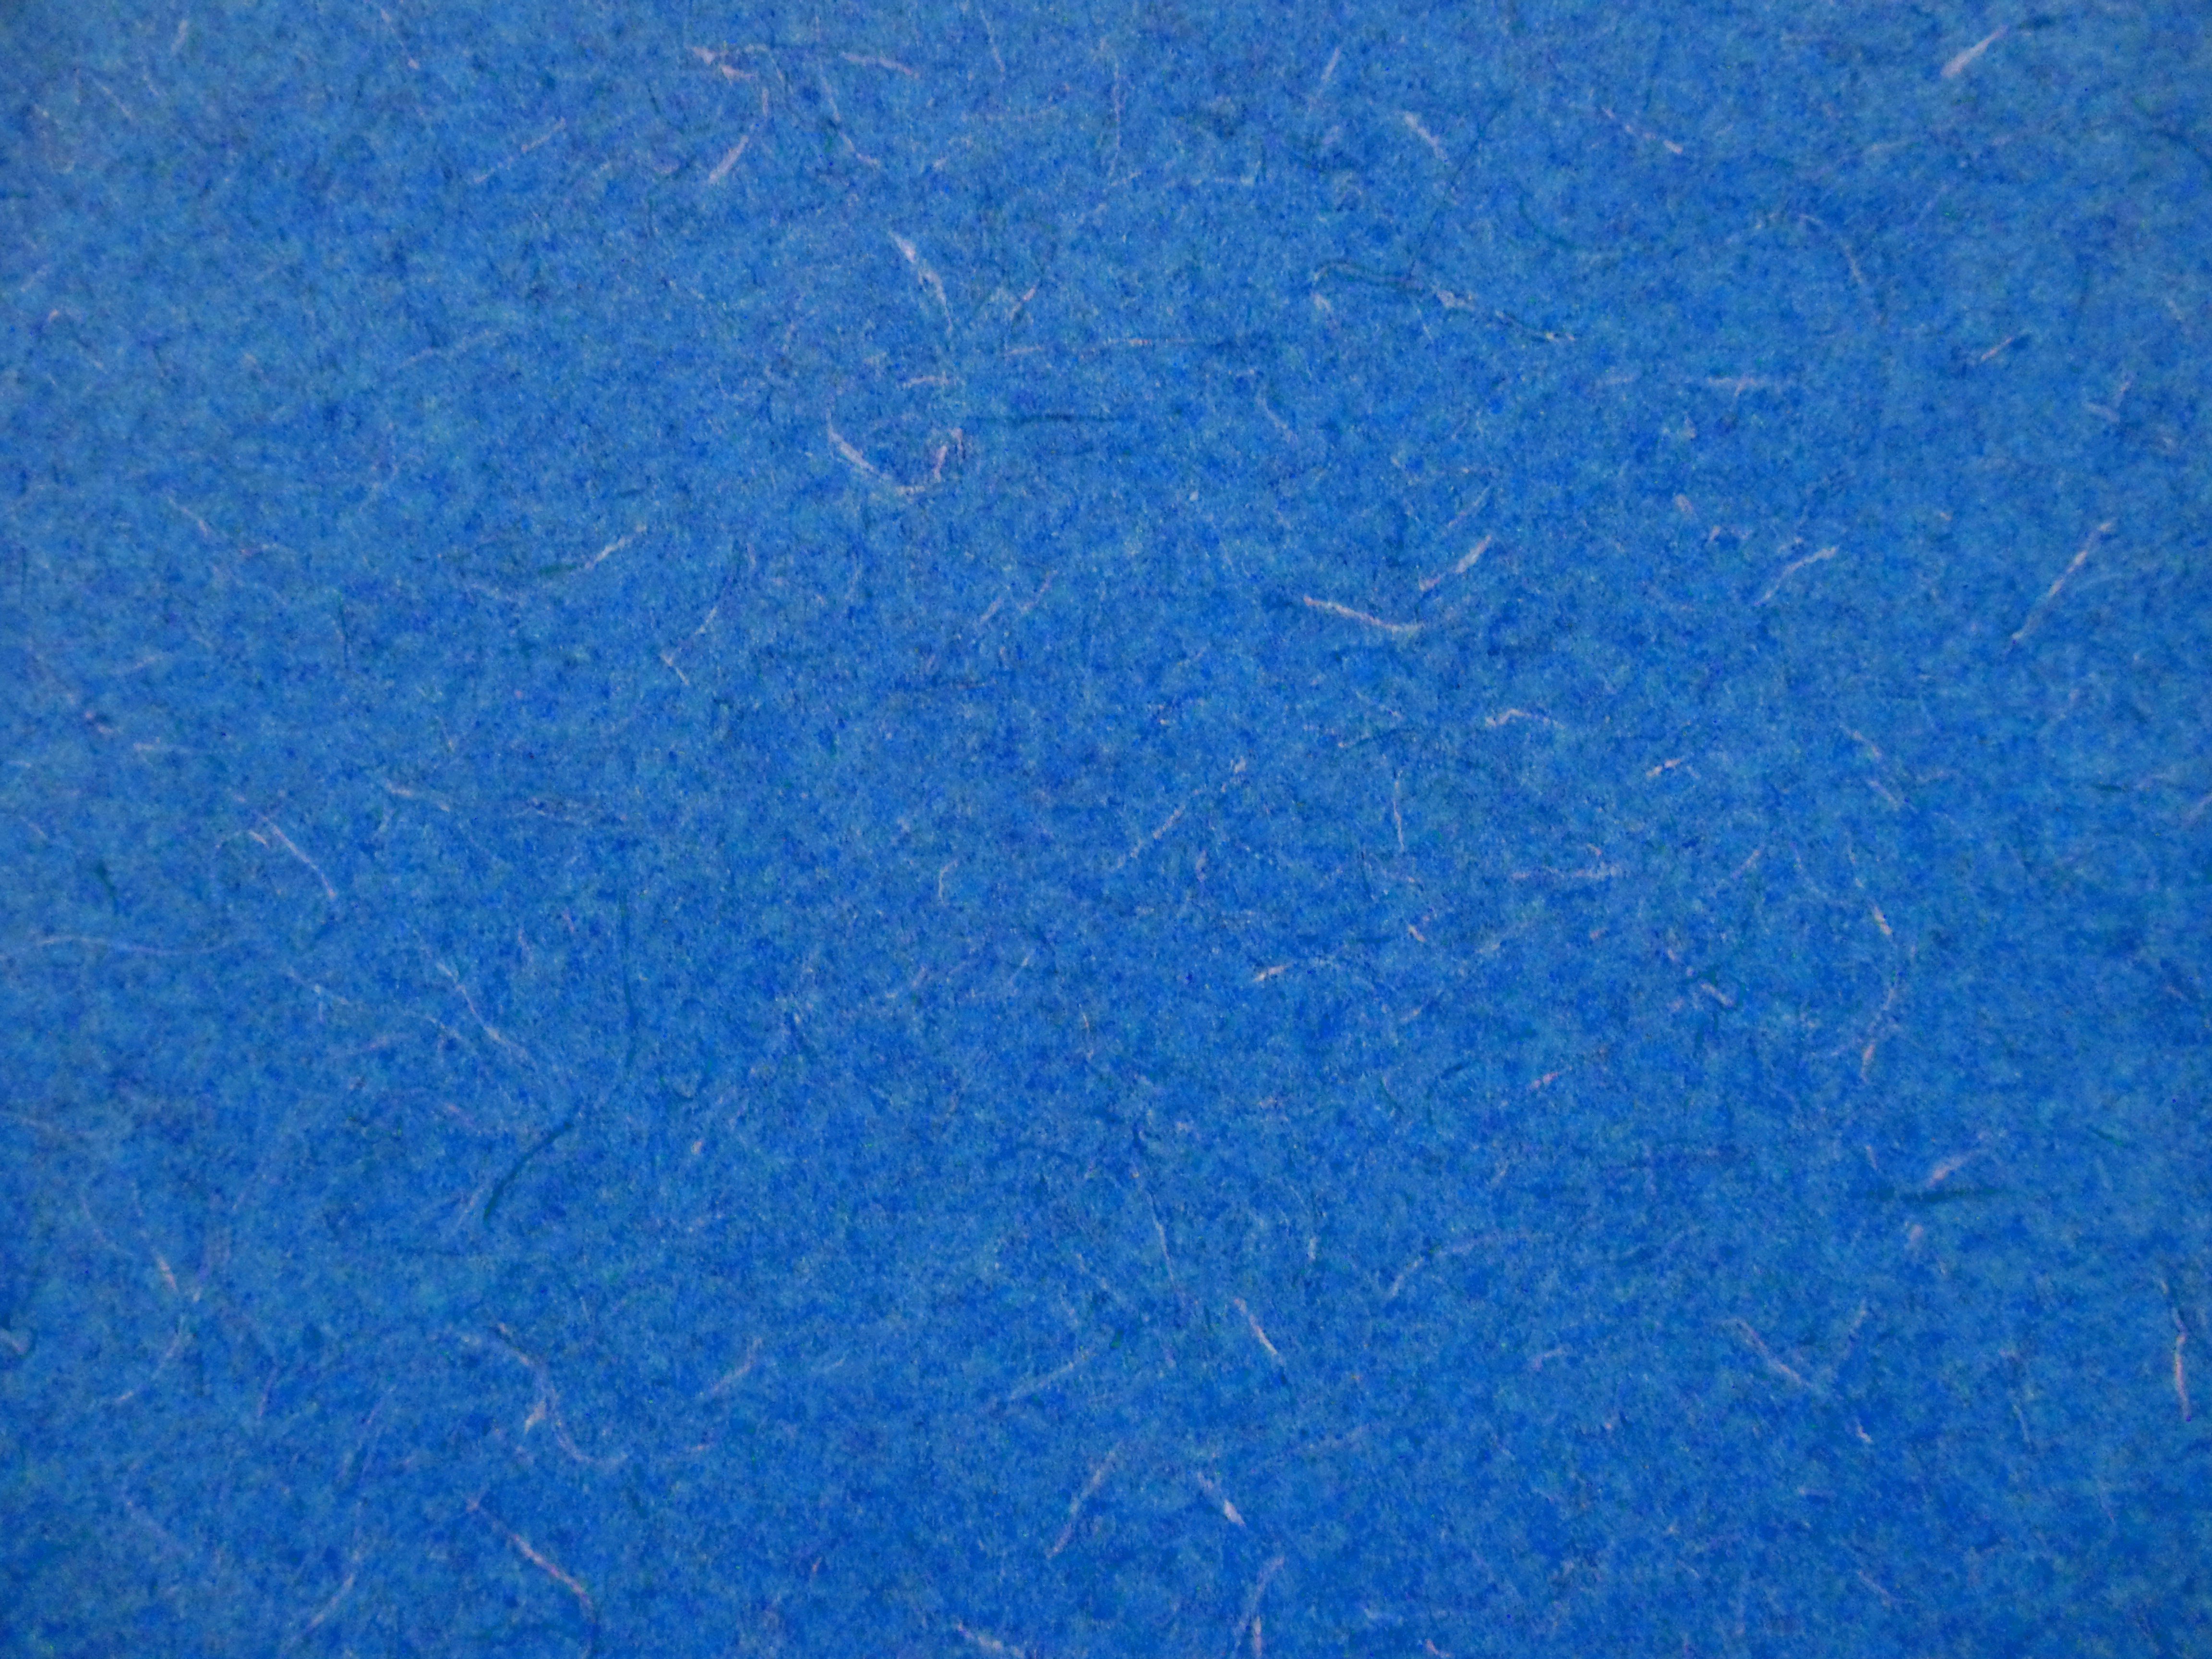
\includegraphics[width=\paperwidth,height=\paperheight]{chapters/images/background-texture-blue.jpg} %higherquality image but too big for overleaf
    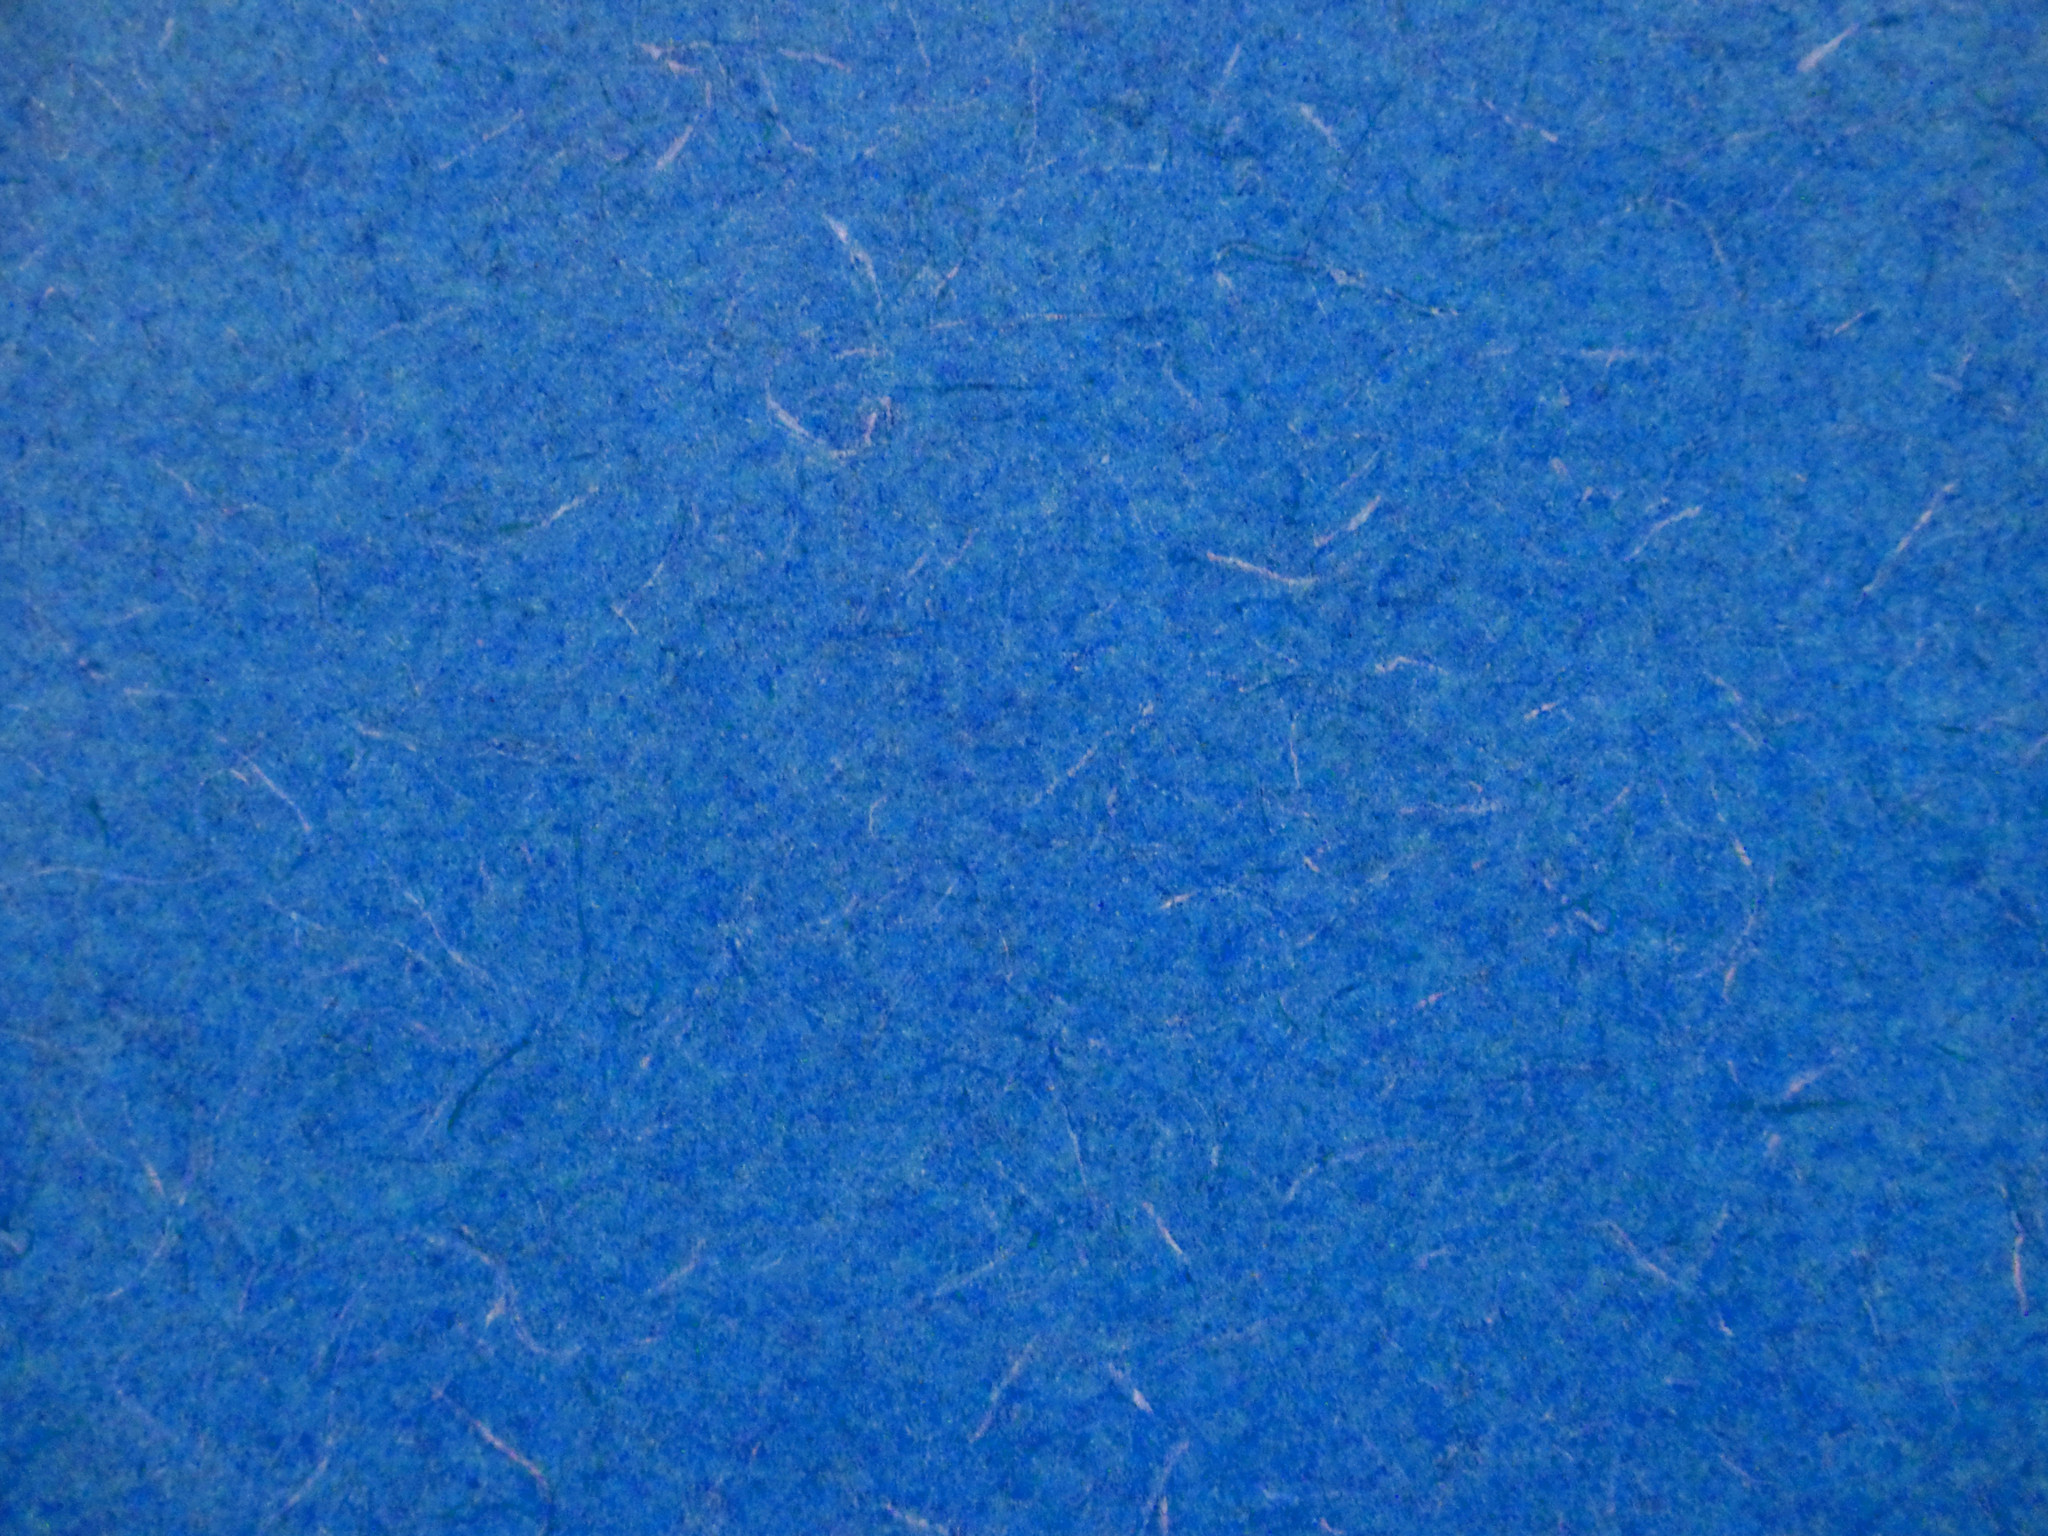
\includegraphics[width=\paperwidth,height=\paperheight]{chapters/images/background-texture-blue-reduced.jpg}
};
\sc
\begin{center}

\color{white}{
\Large Prostate Cancer \normalsize
\vspace{2cm}


I like puzzles. Any type of puzzle. I always have. If I see a puzzle or a problem I have to solve it. I think that is what makes cancer such a fascinating topic for me.

\vspace*{0.5cm}

Imagine you are given a jigsaw puzzle. Now instead of a few hundred pieces, there are several billion pieces. The picture on the box is not a picture of the puzzle inside the box,
it is just a somewhat similar image. Oh, and did I mention there are a whole bunch of pieces missing? and that many pieces are duplicated? Some pieces don't even belong in our box,
but come from a completely different puzzle. On top of that your little sister has spilled paint over some of the pieces so those can't be trusted to contribute to the image. And instead of one
single puzzle, the box contains several, they are all variations of the image on the box, but you have no idea how many different puzzles the box contains. Sound challenging? This is the problem we are solving whenever we sequence a cancer genome.

\vspace*{0.5cm}
\textbf{[Metaphor key]} \\
\textit{puzzle pieces} = sequence reads \\
\textit{picture on box} = reference genome \\
\textit{missing pieces} = hard-to-sequence areas \\
\textit{other puzzles} = contamination \\
\textit{painted pieces} = sequencing errors \\
\textit{multiple puzzles in box} = clonality
}

\end{center}
\end{minipage}
\end{center}



\newpage
\section{Use case 1: Prostate Cancer}

\epigraph{3in}{The time has come in America when the same kind of concentrated effort that split the atom and took man to the moon should be turned toward conquering this dread disease.}{President Richard Nixon}

On December 23, 1971, President Richard Nixon, buoyed by recent technical feats such as the moon landing, signed into law the National Cancer Act, thereby declaring a war on cancer. Today, more than 45 years later, that war is still being waged in full force. While great advancements have been made towards this goal, some of the initial optimism has been quelled by discoveries of the great complexity and heterogeneity underlying cancer.


\subsection{The Hallmarks of Cancer}

Tumor cells evolve from normal cells through the acquisition and accumulation of mutations. The human body has mechanisms in place to repair or dispose of damaged cells and to prevent runaway cell division, so in order for a tumour cell to survive and thrive it needs to acquire changes that provide it with advantages for proliferation and evasion of the cell's defense mechanisms. Evidence suggests this transformation from healthy cells into malignant cells follows a strikingly similar path across all different tumour types \cite{}. A cell's acquired abilities that drive tumour progression are know as the \emph{hallmarks of cancer} and consist of the following six characteristics:

\begin{itemize}
    \itemsep-0.5em
    \item self-sufficiency in growth signals
    \item insensitivity to anti-growth signals
    \item evasion of programmed cell death
    \item limitless replicative potential
    \item sustained angiogenesis
    \item tissue invasion and metastasis
\end{itemize}

Each of these steps overcomes one of the body's anti-cancer defense mechanisms. This evolution into malignancy is an almost darwinian process where the mutations acquired are random, but those cells that have gained mutations which are advantageous for survival will be able to replicate and thrive and accumulate further mutations. Distinguishing the mutations that impart a strategic advantage and thereby \emph{drive} a tumour's progression, from the often huge number of less harmful \emph{passenger} mutations accumulated over the lifetime of a cancer cell is no easy task. The optimal course of treatment for a patient often depends on the mutations present and how the cell functions are subsequently impacted by those mutations. %However, many different mutations may lead to the same disruptions of key pathways, therefore we must evaluate mutations not just at the DNA level but in the broader context of their functional impact on the cell's internal processes.



\subsection{Cancer's Complexities}

Determining the exact genetic sequence of healthy individuals is already quite a challenging endeavor; trying to extend this to cancer genomes takes this challenge to the extreme. There are several complexities present in cancer geneomes that make accurate determination of the genetic changes and their downstream impacts a difficult task. In the following sections we will discuss some of these complexities and explore the biological and informatics challenges they pose.

\subsubsection{The Bio}
\paragraph{Small variants} comprise the simplest class of mutations; those consisting of alterations of just a handful of bases, for instance the \emph{substitution}, \emph{deletion} or \emph{insertion} of one or more nucleotides.

The impact of such mutations depends on where in the genome they occur. Single nucleotide variants (SNVs) in exonic regions can range from having no effect on the resulting protein (silent), to changing an amino acid in the protein to a different amino acid (missense mutations), to changing a codon into a stop codon (nonsense mutation) which nearly always results in a nonfunctional protein. If this happens in a protein that is vital to the functioning of the cell this can have disastrous consequences <some examples of SNVs causing serious problems/phenotypes>

While variants within the coding sequence are most likely to have an impact on cell health, small variants \emph{outside} the coding sequence can also have drastic impact on health; for example, 70\% of melanomas exhibit a point mutation in one of two positions in the promoter region of TERT (Horn et al. 2013; Huang et al. 2013), suggesting such somatic point mutations in regulatory regions may play a role in tumorigenesis.

\paragraph{Structural variations (SVs)} are larger-scale mutations involving rearrangement of segments of DNA of more than roughly 50 bp. In some cases, these rearrangements can cause (parts of) two genes that are usually separated by some distance on the genome to come together to form new hybrid genes, which may be transcribed into fusion proteins, and which have a potentially disastrous effect on cell processes. The text book example of such a gene fusion is the so-called Philedelphia fusion frequently observed in leukemia \cite{TODO}. In this Philedephia chromosome, a translocation between chromosomes 9 and 22 leads to a fusion of the BCR and ABL1 genes. This fusion gene is expressed, and the aberrent fusion protein causes disruptions to key signalling pathways governing the cell cycle, causing the cells to divide uncontrollably and thereby drive tumor progression. Accurate detection of such structural variations is crucial, as they may serve as diagnostic markers \cite{nowell1960chromosome,nowell1961chromosome} or even therapeutic targets \cite{druker2001activity, druker2001efficacy}.

SVs often occur outside coding regions, but this does not diminish their potention for great impact, for instance by disruption of the regulatory mechanisms of tumour supressor genes or oncogenes \cite{TODO}. These types of SVs not involving coding regions directly, may only be detected through whole-genome sequencing.

%Numerous fusion genes have been found to play a role in tumorigenesis \cite{TODO},
%in prostate cancer the TMPRSS2-ERG fusion is present in roughly 40\% of tumours, \cite{TODO}

\paragraph{Clonality} refers to the phenomenon that cells in different physical areas in a tumour may be genetically very distinct. As a cell obtains a mutation that is beneficial to proliferation, it may instigate a new cluster, or \textit{clone}, of genetically similar cells while in other areas of the tumour cells may follow a different evolutionary path and create genetically different subclones. When sequencing a tumour, DNA from different cells -and thus potentially very different genomes- is mixed together and sequenced as one. Reconstructing the different clonal genomes from this data is immensely challenging.

\paragraph{Further complexities} in the analysis of cancer genomes include the temporally evolving nature of tumours; performing the same sequencing experiment on the same tumour at different points in time will often yield a very different picture as the composition of the tumour and the acquired mutations will have changed. This further complicates the process of comparing different samples and elucidating key characteristics that have the potential to aid in the diagnosis and treatment of patients. Furthermore, studies in epigenetics have shown that tumorigenesis is not solely driven by mutations in nucleotide sequence, but secondary alterations such as DNA methylation may have an equal if not greater impact \cite{TODO}.

\subsubsection{The Informatics}

All these complexities in the biology of cancer gemomes translate to complexities of the downstream informatics analysis pipelines.


We know that changes in sequence and structure of DNA contributes to cancer development. But how do we describe these properties? Any two healthy individuals differ greatly in their DNA sequence; it's what makes us us. How to denote these differences is a non-trivial problem, as is determining which of these differences are just part of the natural variation between individuals and which are ones detrimental to our health and functioning.

If you were asked to describe the differences between two Shakespeare plays, how would you go about it? They are made up of the same alphabet, and share many of the same words and even whole sentences, but to list the differences between them can be done in many ways. You could number the words in both books and take note of the ones that are different in each position, but then if you were to take two identical sentences and prefix one with a single extra word, all positions would end up being flagged as different while clearly these sentences are nearly identical. And ..

<note: ditch the book analogy? example shakespearean sentence to illustrate? >

poor concordance between variant callers: https://genomemedicine.biomedcentral.com/articles/10.1186/gm432


Currently variations in DNA are described relative to a \emph{reference genome}; a sequence intended to represent the \emph{average} human genome, which was constructed by taking the most frequently observed nucleotide at any given  position in the genome
<discuss some drawbacks/things to realize: based on relatively small set of samples, not optimally diverse set of individuals>

\begin{comment}
As we have seen, the choice of software can impact downstream analysis, and variant calling is no exception. Different aligners employ different mapping strategies, which leads to different variant calls for the same observed sequence depending on the choice of algorithm, complicating variant comparisons between studies \cite{zook2014integrating}. While there do exist tools to canonicalise some of these differing representations \cite{vcflib}, complex variants remain that do not have a single obvious standard form (Figure \ref{fig:variant-multiple-representations}).
But even for the simpler cases, there is not always a clear consensus on how to standardise representation. Consider for instance the case where an adenine nucleotide has been inserted, transforming the sequence \verb+TAAG+ to \verb+TAAAG+. Do we describe the insertion to have happened at position 1 (after the \verb+T+), position 2 (between the two \verb+A+s), or at position 3 (before the \verb+G+)? While this particular case is easily solved by agreeing on a convention of either left-aligning or right-aligning these variants, such community agreement does not currently exist, with most next-generation analysis tools opting for left-alignment, while certain variant databases such as HGVS [TODO cite] still recommend (but do not enforce) alignment to the position nearest the 3\` end of the gene \cite{hgvs-position}, which translates to right-alignment in genomic coordinates for reverse strand genes. Furthermore, once variants have been submitted to online databases, information about surrounding variants observed in the same sample is often not kept, making it impossible to resolve equivalency of variant representations going forward.
\end{comment}


\begin{figure}[h!]
    \centering
    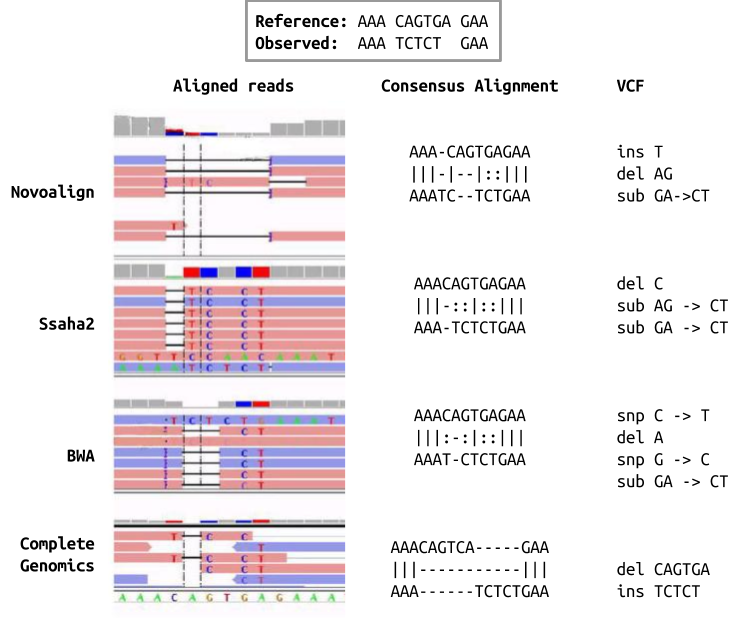
\includegraphics[width=400pt]{chapters/images/variant-representation-all.png}
    \begin{comment}
        image in google drive https://docs.google.com/drawings/d/1WWmzW6uWtJ7HZ5WVgtg_oAMA_3E_569M4Ikjz4Ecjic/edit
    \end{comment}
    \caption{Complex variants can be represented in multiple ways. Four different aligners (Novoalign, Ssaha2, BWA, Complete Genomics) treat the same variant in vastly different ways, which leads to such differing sets of variant descriptions in the VCF files that it is no longer apparent that these variants in fact describe the same observed sequence.}
    \label{fig:variant-multiple-representations}
\end{figure}


<not to mention sequencing errors, at rate of abt x/100, sequencing depth helps but tradeoff with cost>

sources of mismatch with reference genome \\
- real mutation \\
- wrong base call \\
- wrong mapping/variant call \\


<repetitive regions>

The result of all of this is that different variant calling tools will produce different sets of variants given the exact same input dataset and reference genome, and it is hard to know who does a better job, if their respective papers are to be believed each one of them far outstrips all the others. But as with everything in life, the truth lies somewhere in the middle. Each of the variant callers has its strengths and weaknesses, some may very accurate in calling one type of variant but have  more difficulty with others. Some are very accurate in healthy genomes but less so in highly mutated genomes or vice versa. One possible solution is to run a set of variant callers

\paragraph{Structural variations}
<very very poor overlap between different methods>

<hard to resolve exact location of junctions>

<chainfinder>
\paragraph{Clonality}
\paragraph{Temporal Evolution}
\paragraph{Epigenetics}



\newpage
\thispagestyle{empty}
\begin{center}
\vspace{2cm}
\begin{minipage}{5in}
\tikz[remember picture,overlay]
\node[opacity=0.8,inner sep=0pt] at (current page.center){
    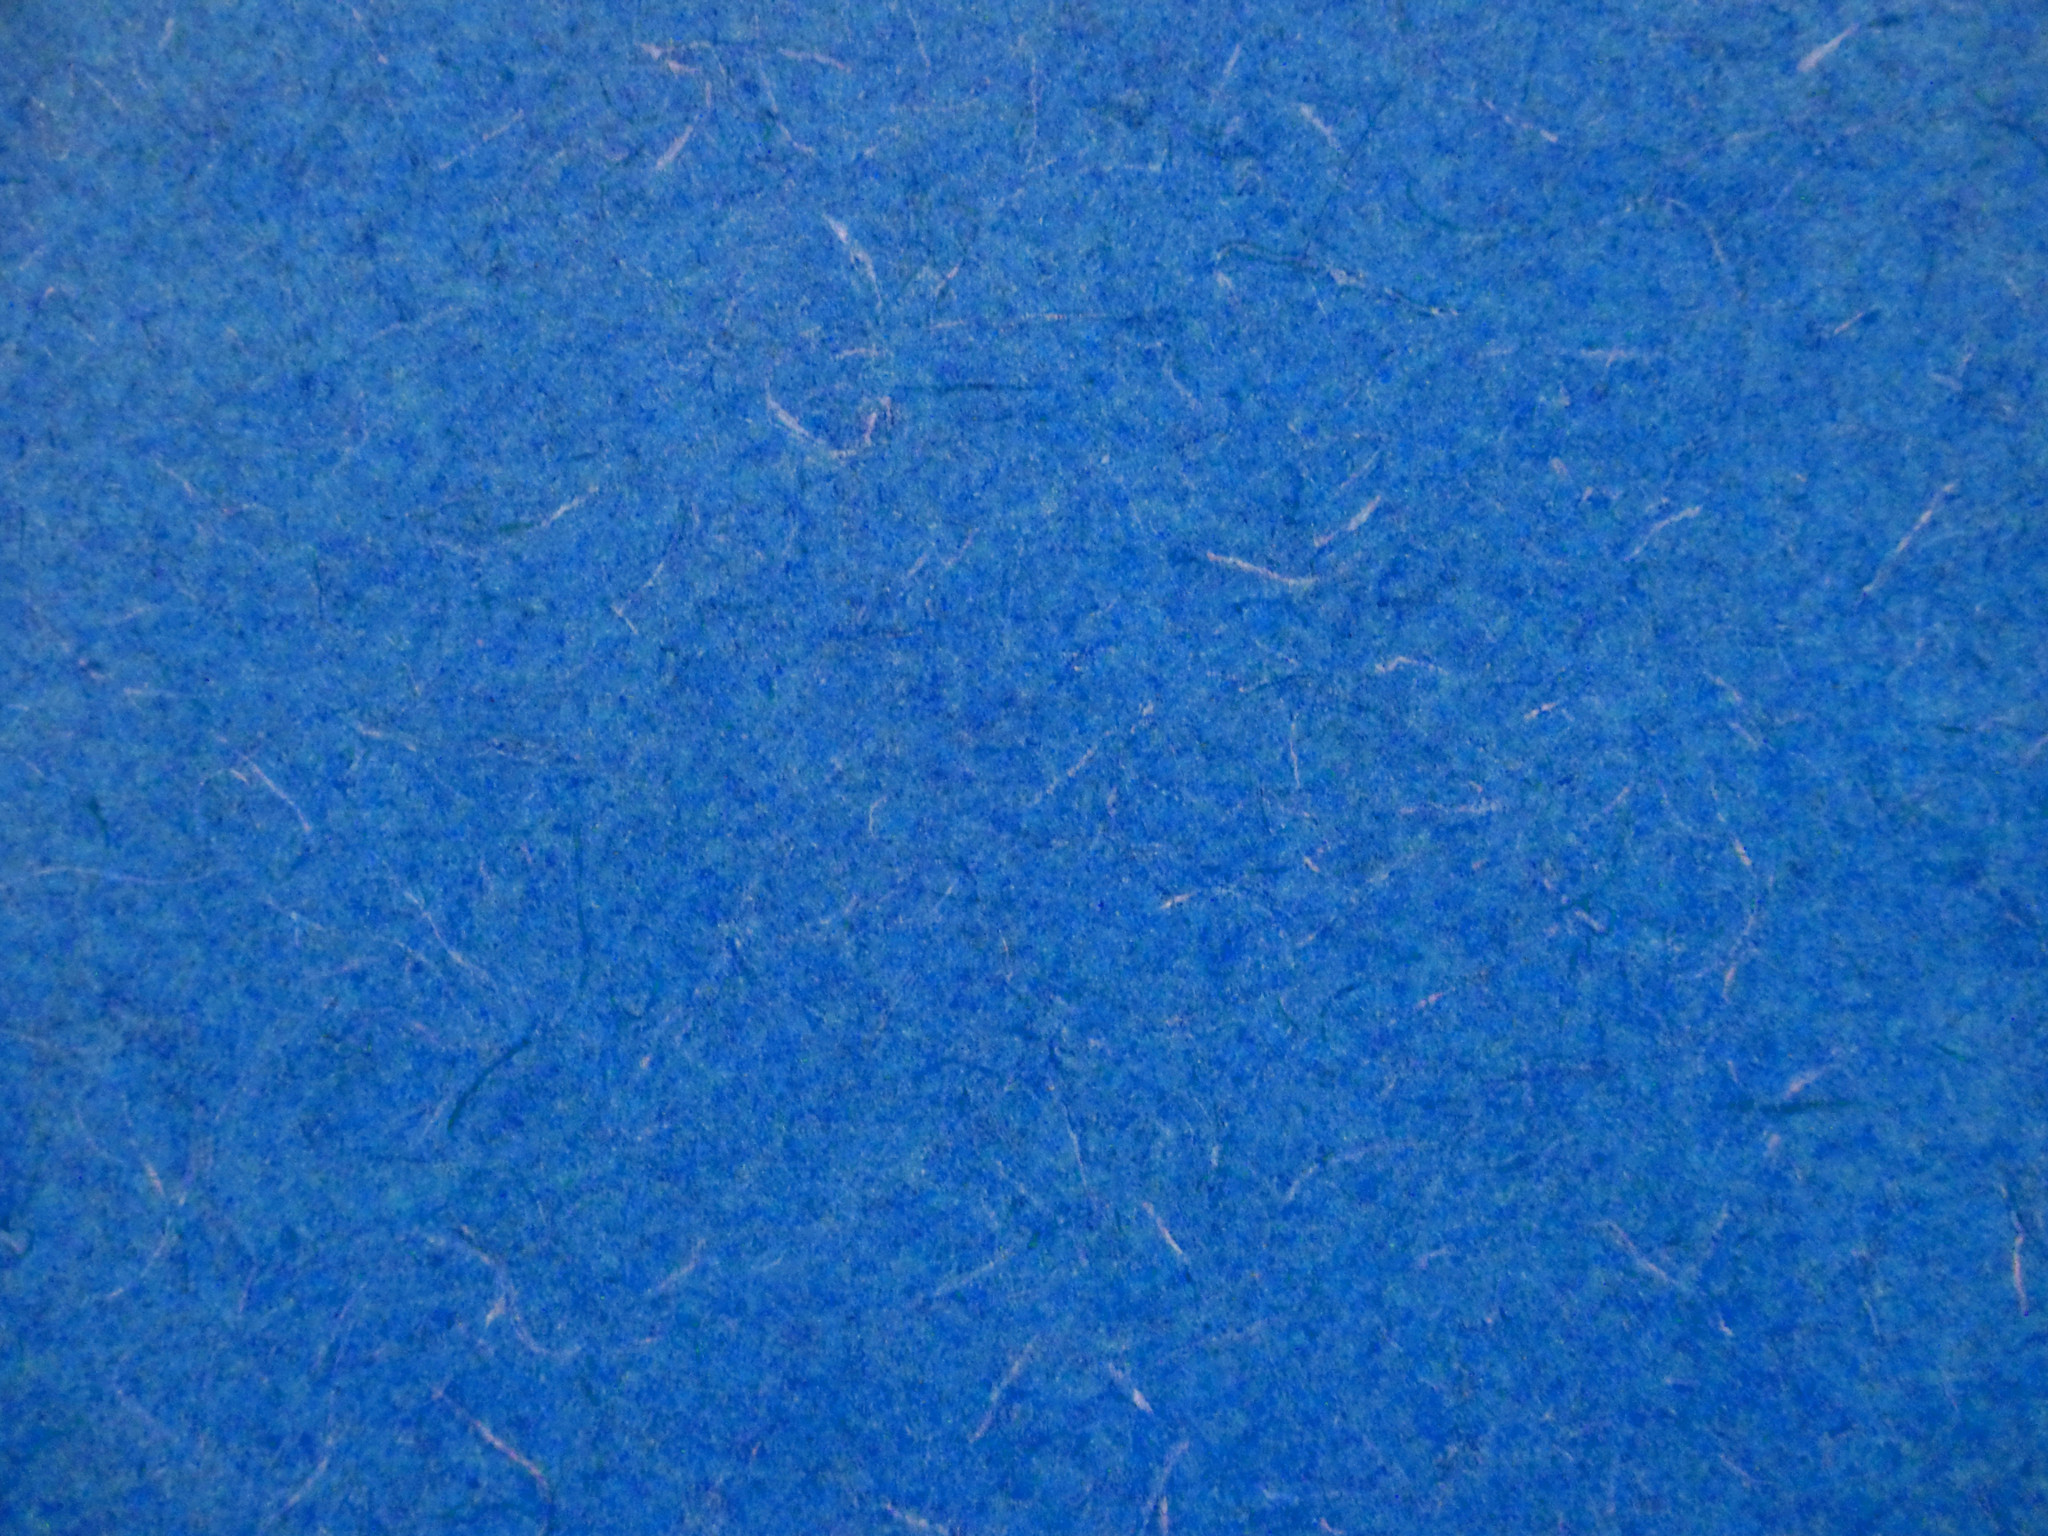
\includegraphics[width=\paperwidth,height=\paperheight]{chapters/images/background-texture-blue-reduced.jpg}
};
\sc
\begin{center}

\color{white}{
\Large The Human Microbiome \normalsize
\vspace{2cm}

When Dutch inventor and scientist Antonie van Leeuwenhoek first turned his microscope to a drop of rain water and discovered within a wealth of microscopic life which he termed \textit{animalcules}, a whole new world of knowledge opened up. Soon after, it was discovered that while these organisms might be microscopic in size, their impact on human lives was enormous, causing food to spoil and disease to spread. Through the study of these micro-organisms, scientists were able to develop methods for enhanced food preservation and eventually also new treatments and vaccines for a whole range of illnesses.

Cost of sequencing has now dropped enough that it has become feasible to sequence not only a patient's own DNA, but also the DNA of their microbiome to make a diagnosis or to determine the best treatment option.




\vspace*{2cm}
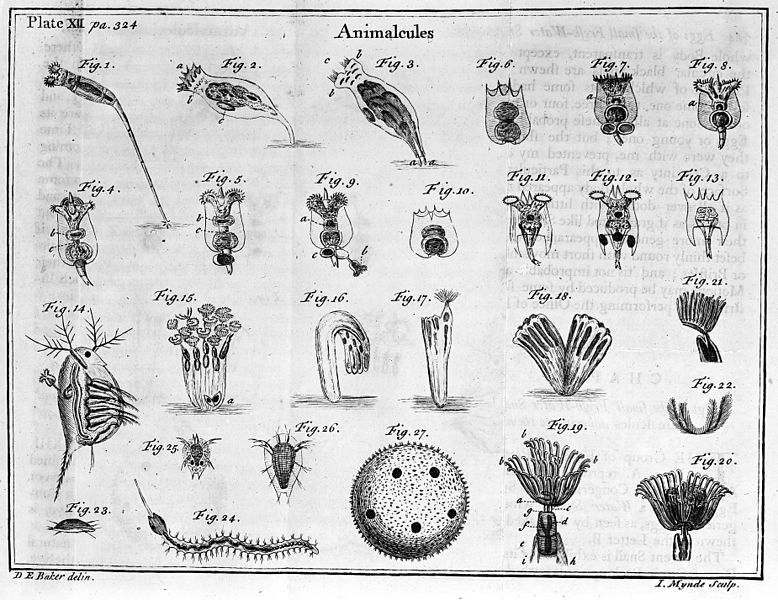
\includegraphics[scale=2]{chapters/images/mycrobiota/animalcules2.png}

}

\end{center}
\end{minipage}
\end{center}

\newpage


\section{Use case 2: Microbiota}

\begin{comment}

overview of reading materials about the human microbiome

http://www.richardsprague.com/note/2017/10/16/best-academic-papers-about-the-microbiome/

informal history of microbiology: https://www.bioexplorer.net/history_of_biology/microbiology/
\end{comment}

\subsection{The Bio}
first complete bacterial genomes published in 1995  \cite{land2015insights}

16S rRNA

whole genome shotgun

\subsection{The Informatics}


\begin{comment}
history of microbiolgy: https://courses.lumenlearning.com/boundless-microbiology/chapter/introduction-to-microbiology/

<WGS reveals changes outside coding regions, such as one affecting regulation of genes are of importance, and can reveal large scale changes (SVs), fusion genes>

<epigenetics>

<potential of developing treatments from all this knowledge>

sources:
- Hallmarks of cancer: the next generation [@hanahan2011hallmarks]
- Chromosome aberrations in solid tumors [@albertson2003chromosome]

~~~
low-resolution methods:
- fluorescent in sit hybridisation FISH [Pinkel et al 1988, Thompon and Gray, 1993]
- chromosome painting [Jauch et al, 1992]
- spectral karyotyping [Schrock et al 1996]
- comparative genome hybridisation CGH [Kallioneimi 1992]

- arrays

high-throughput:
 - LOH [@hampton1996simultaneous]
 - GWAS

 - 2003 still infeasible to sequence entire tumor genome, so
   ESP (end sequencing profiling) used [Volik et al 2003]
       (- BAC library from tumor, sequence ends, map to reference)
    → reconstruction from ESP data [Rapael et al 2003]

now: WGS
- NGS: DNA short reads
- NGS: RNA Seq
- NGS: Paired end mapping [@korbel2007paired]
- limitations of current methods
~~~

advanced in cancer research specifically from next generation methods: [@meyerson2010advances]

\end{comment}







\begin{comment}

types of SVs: standard, complex, chromothripsis [@stephens2011massive]

- well-known examples
    - TMPRSS ERG
    - ABL gene on chr9, chronic myeloid leukema, translocation between chr9 and 22,
       changes regulation, promotor becomes promotor of BCR gene on chr22
      [Heisterkamp et al 1983]

#### usefulness in biomarker and treatment development

- Gleevec, targeting BCR-ABL fusion gene [@druker2001efficacy]
- Herceptin, targeting ERBB2 amplification [@kauraniemi2004effects]


#### SV Tools and databases

~~~
- catalogued in Mitleman database [Mitelman 2003]
- COSMIC
- ..
~~~

## Clonality

## Temporal evolution

## etc..
~~~
<Informatics/analysis methods>
 - History of methodologies (gwas, ..)
 - NGS: Huge datasets, excel and manual analyses no longer suffice
 - Cancer: Germline correction, drivers vs passengers

<Limitations of current methods>
 - imperfect data
 - disagreements and biases per lab/informatics technique

<Challenges in tumour genome reconstruction>
→ explain in biology section, here describe why that complicates things

 - Normal Contamination
 - Clonality detection
 - Event Chains detection
 - Temporal evolution detection


\end{comment}

\section{Scope of this Thesis}
Bioinformatics is a vital part of many fields of research. While these may differ greatly in the biology involved, many of the bioinformatics concepts are shared among them. In \hyperref[chapter:general]{Chapter \ref{chapter:general}} we discuss several such widely-applicatble bioinformatics projects. Galaxy for reproducible analysis workflows, iReport for results reporting withing Galaxy. (Circos? myFAIR?)



\bibliographystyle{ieeetr}
\bibliography{references}

\begin{savequote}[75mm]
Nulla facilisi. In vel sem. Morbi id urna in diam dignissim feugiat. Proin molestie tortor eu velit. Aliquam erat volutpat. Nullam ultrices, diam tempus vulputate egestas, eros pede varius leo.
\qauthor{Quoteauthor Lastname}
\end{savequote}

\chapter{Technical: iReport, myFAIR, Circos?, Training?}
\setcounter{figure}{-1}
\setcounter{table}{-1}
\setcounter{section}{-1}
%\setcounter{enumiv}{-1}
\setcounter{NAT@ctr}{-1}

\newthought{There's something to be said} for having a good opening line. Morbi commodo, ipsum sed pharetra gravida, orci  $x = 1/\alpha$ magna rhoncus neque, id pulvinar odio lorem non turpis \cite{Eigen1971, Knuth1968}. Nullam sit amet enim. Suspendisse id velit vitae ligula volutpat condimentum. Aliquam erat volutpat. Sed quis velit. Nulla facilisi. Nulla libero. Vivamus pharetra posuere sapien. Nam consectetuer. Sed aliquam, nunc eget euismod ullamcorper, lectus nunc ullamcorper orci, fermentum bibendum enim nibh eget ipsum. Donec porttitor ligula eu dolor. Maecenas vitae nulla consequat libero cursus venenatis. Nam magna enim, accumsan eu, blandit sed, blandit a, eros.
$$\zeta = \frac{1039}{\pi}$$

\verb+short intro to chapter tying the different papers together +

% For an example of a full page figure, see Fig.~\ref{fig:myFullPageFigure}.
\newpage

%%%%%%%%%%%%%%%%%
%    iReport
%%%%%%%%%%%%%%%%%

\articletitle{iReport: A generalised Galaxy solution for integrated experimental reporting}
Saskia Hiltemann\textsuperscript{\ref{affil:emc-bioinf},\ref{affil:emc-urology}},
Youri Hoogstrate\textsuperscript{\ref{affil:emc-bioinf},\ref{affil:emc-urology}},
Peter van der Spek\textsuperscript{\ref{affil:emc-bioinf}},
Guido Jenster\textsuperscript{\ref{affil:emc-urology}},
Andrew Stubbs\textsuperscript{\ref{affil:emc-bioinf}}

\small
\begin{enumerate}
\itemsep-0.5em
\item Department of Bioinformatics, Erasmus Medical Center, Rotterdam, The Netherlands. \label{affil:emc-bioinf}
\item Department of Urology, Erasmus Medical Center, Rotterdam, The Netherlands. \label{affil:emc-urology}
\end{enumerate}
\normalsize


Published in: GigaScience \\
DOI: \url{https://doi.org/10.1186/2047-217X-3-19} \\

\section*{Abstract}

\textbf{Background:} Galaxy offers a number of visualisation options with components, such as Trackster, Circster and Galaxy Charts, but currently lacks the ability to easily combine outputs from different tools into a single view or report. A number of tools produce HTML reports as output in order to combine the various output files from a single tool; however, this requires programming and knowledge of HTML, and the reports must be custom-made for each new tool.\\
\textbf{Findings:}We have developed a generic and flexible reporting tool for Galaxy, iReport, that allows users to create interactive HTML reports directly from the Galaxy UI, with the ability to combine an arbitrary number of outputs from any number of different tools. Content can be organised into different tabs, and interactivity can be added to components. To demonstrate the capability of iReport we provide two publically available examples, the first is an iReport explaining about iReports, created for, and using content from the recent Galaxy Community Conference 2014. The second is a genetic report based on a trio analysis to determine candidate pathogenic variants which uses our previously developed Galaxy toolset for whole-genome NGS analysis, CGtag. These reports may be adapted for outputs from any sequencing platform and any results, such as omics data, non-high throughput results and clinical variables.\\
\textbf{Conclusions:} iReport provides a secure, collaborative, and flexible web-based reporting system that is compatible with Galaxy (and non-Galaxy) generated content. We demonstrate its value with a real-life example of reporting genetic trio-analysis.


\section*{Findings}

Structured reporting and documentation of experimental outcome is required for the successful transfer of knowledge from the research scientist to their peers and to the broader academic community.

Galaxy is a platform that aims to provide complex bioinformatics services and tools in an easy-to-use web-based graphical user interface \cite{goecks2010galaxy,blankenberg2010galaxy,giardine2005galaxy}. The output from these tools can be displayed using built-in Galaxy visualisation applications \cite{goecks}, via specialised visuals implemented as a component in the workflow deployed in Galaxy \cite{cgtag} or by downloading the results and visualising the output with applications external to Galaxy (e.g., Excel, TIBCO spotfire, R, spreadsheet programs, \emph{etc}).

Galaxy has the capacity to track the provenance of the source data, the workflow, as well as the workflow components used to analyse the data. Currently users can share their workflow and results within Galaxy, but do not have access to a simple method to summarise results from multiple tools and/or workflows in an integrated report. To address this issue we have developed iReport, an integrated reporting application that provides users with a flexible means to produce dynamic HTML reports which can be shared with other Galaxy users or downloaded to disk.

Systems used by end-users to deliver graphical output range from open-source applications, such as \emph{Ad Hoc} reports \cite{url-adhoc}, Google charts (and docs) \cite{url-googlecharts} and OpenOffice \cite{url-openoffice}, to commercial applications such as Microsoft Office.
Indeed scientific reporting applications both open-source (Bioconductor \cite{url-bioconductor}, Circos \cite{circos}\cite{url-circos}) and commercial software (e.g., Omniviz \cite{url-omniviz}, Partek \cite{url-partek}) include a multitude of visualisation capabilities with a focus on data reporting and presentation of data in the context of the experimental design and with associated meta-data.
There are some applications, like TIBCO spotfire \cite{url-spotfire}, which are capable of integrating results from multiple sources including associated text and meta-data and other applications which serve as an electronic lab note book (e.g., IDBS \cite{url-idbs}).
Additionally there have been many products developed to address the selection and reporting of variants for pathogenic variant selection including the workflow to identify those variants (e.g., Gensight \cite{url-gensight}, Cartagenia \cite{url-cartagenia}, Clincial Genomicist \cite{clinicalgenomist}).
For data generated in R, dynamic reporting packages such as KnitR \cite{url-knitr}, Sweave \cite{sweave} and R-Markdown \cite{url-rmarkdown}, allow for the integration of data-generating code within the report specification itself. Similar systems exist for other programming languages, for example Tangle \cite{url-tangle} (JavaScript), Active Markdown \cite{url-activemarkdown}(CoffeeScript) or IPython Notebooks \cite{url-ipythonnotebook} (Python).
These are very versatile tools, but require programming knowledge to use effectively. iReport offers an open-source application for both Galaxy and non-Galaxy produced results allowing for the generation of customized integrated reports for any type of project or workflow.
The advantage to Galaxy users is that the output from any application can be included into any report, and that a report template can be reused for other projects.
Also, the report may be securely shared with one or many users of that Galaxy instance or made publicly available. iReports can be completely configured from the tool web interface, and requires no programming or knowledge of the underlying system.

We demonstrate iReport’s utility through an example where a genetic report is generated from outputs of an existing Galaxy next-generation sequencing (NGS) toolkit, CGtag \cite{cgtag}. iReport can also be used as an electronic lab notebook by creating an iReport which links out to various other iReports containing different analysis reports from various samples. It can be also be coupled to output from other Galaxy instances, for example output generated by specialized Galaxy instances such as Confero \cite{confero}, ORIONE \cite{orione}, and Galaxy-P \cite{url-galaxyp}.

\section*{Functionality}
iReport dynamically generates HTML, and employs JavaScript and jQuery to create interactive components, such as searchable, sortable, paginated tables and zoomable images. iReport is ideally suited to use as the final step in a workflow; the pipeline developer configures the report once and end-users are then presented with a templated report each time users run the workflow, while only needing to provide the input files for the pipeline \cite{CGtagpipeline}. iReport can also be used directly by end-users as a means of easily sharing their results with other Galaxy users, or the public via Galaxy's native sharing capabilities.

The generic reporting functionality and usage of iReport is outlined below using an example iReport created for the recent Galaxy Community Conference, which is also available for viewing online \cite{url-ireport-tutorial}. It is followed by an example of a genetic report that can be used for trio analysis, which can easily be modified for any trio reporting or extended to quartets or larger families, also available from our demo galaxy \cite{url-genetic-ireport}.

\section*{iReport Structure}

iReport produced a report webpage consisting of one or more subpages with one or multiple elements included on each subpage. The primary output of iReport is:


\begin{enumerate}
 \item A cover page
  \begin{enumerate}
    \item Title of the report
    \item Cover image
  \end{enumerate}
 \item Main report page consisting of a set of tabs. Each tab consisting of one or more \emph{content items}. Each content item can be one of the following types:
  \begin{enumerate}
    \item Text
    \item Images
    \item Tables
    \item PDF Files
    \item Links
  \end{enumerate}
\end{enumerate}

An iReport tutorial has been developed to demonstrate and explain the functionality of iReport, and is available as a shared history from the CTMM-TraIT public Galaxy instance \cite{url-ireport-tutorial}. The following sections describe each of the components of iReport in more detail.

\subsection*{Cover Page}
The cover page consists of a user-specified title and a cover image. The cover image parameter is optional and when the field is left blank a default image is used (\hyperref[fig:defaultcover]{Figure \ref*{fig:defaultcover}}).
By clicking on the image, or the link above it, the user can access the main report page. There is also a link to download the entire iReport webpage, including all dependency files, for storing or viewing on different systems.

\begin{figure}[h!]
    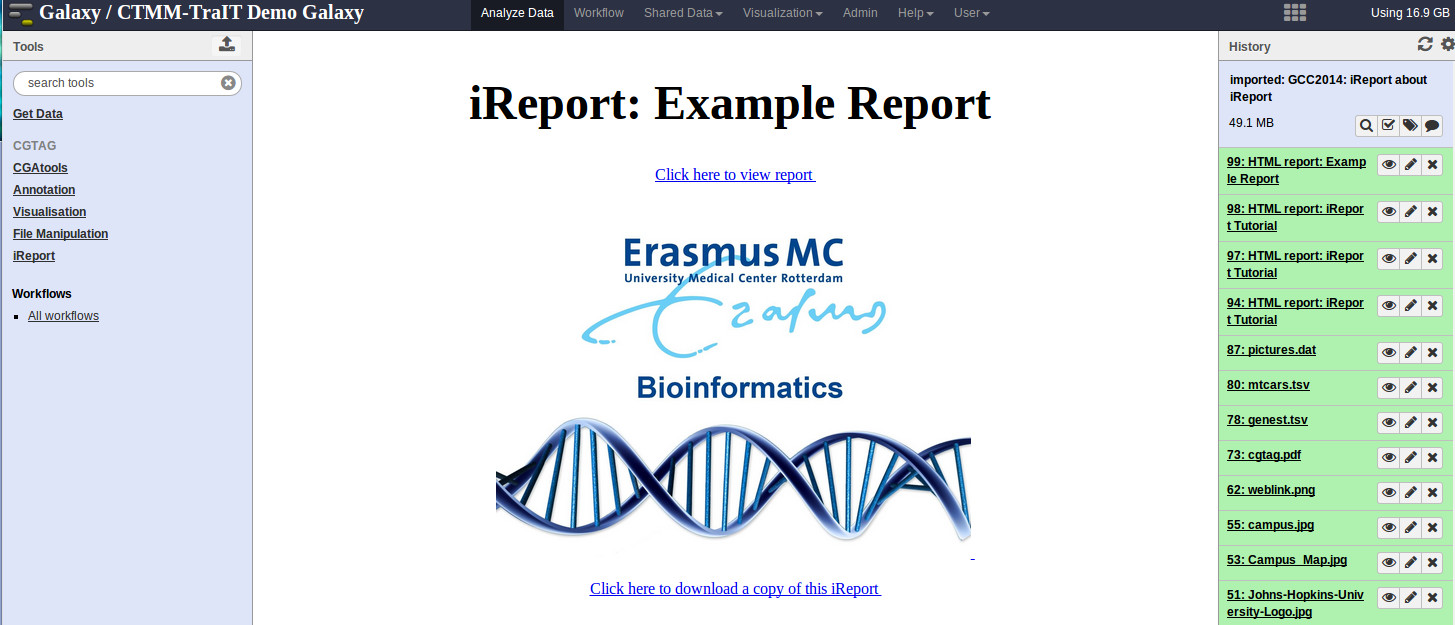
\includegraphics[width=\textwidth]{chapters/images/iReport/Hiltemann_defaultcover.jpg}
    \caption{Example cover page.Example of a cover page with title \emph{Example Report} and the default cover image. A link to download the entire iReport web page is also provided.}
    \label{fig:defaultcover}
\end{figure}


\subsection*{Main Report Page}
An arbitrary number of tabs may be added via a repeat parameter. Each tab can be labelled with a name specified by the user. An arbitrary number of \emph{content items} may then be added to each tab in a repeat parameter. A type must be specified for each content item (e.g., text, image, table \emph{etc.}), as well as several other parameters depending on the type chosen (\hyperref[fig:wrapper]{Figure \ref*{fig:wrapper}}). Layout is mostly left up to the browser, but users can explicitly add a line-break after each item to force items to appear underneath each other.

% Galaxy wrapper
\begin{figure}[h!]
    \centering
    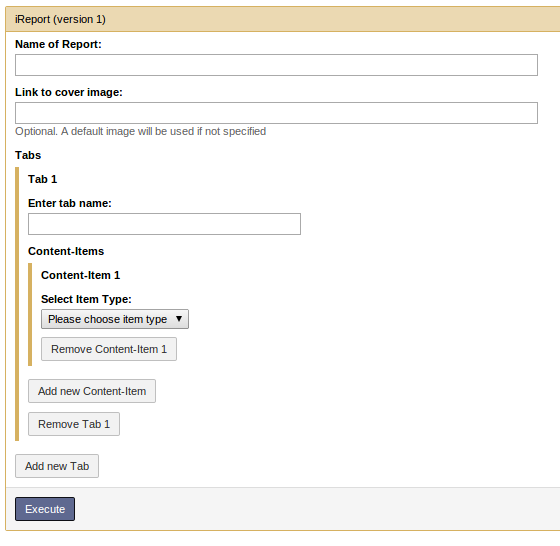
\includegraphics[scale=0.5]{chapters/images/iReport/Hiltemann_wrapper.jpg}
    \caption{iReport tool wrapper. iReport's tool interface. Minimally a report title and at least 1 tab with 1 content item need to be specified.}
    \label{fig:wrapper}
\end{figure}

\paragraph*{Content item: Text Field}
Text can be entered in a text field in the tool interface, for example to create an introduction paragraph and to give a description of the items on the page. Text is printed verbatim, although a small number of HTML tags are allowed in order to give the user some control over formatting (e.g., \verb+b, i, em, strong, h1-h6+ tags). Text files can also be specified, and the contents of the file will be printed to the screen verbatim.

\paragraph*{Content item: Images}
Many tools produce images as output, which can also be displayed by iReport. Users specify the image file from their Galaxy history, and the desired image size. For images that have been scaled down, an optional jQuery zoom-on-mouseover effect may  be added (\hyperref[fig:imagezoom]{Figure \ref*{fig:imagezoom}})\cite{url-jqueryzoom}. Currently supported image formats are JPG, PNG and SVG.

%% zoomeffect
\begin{figure}[h!]
    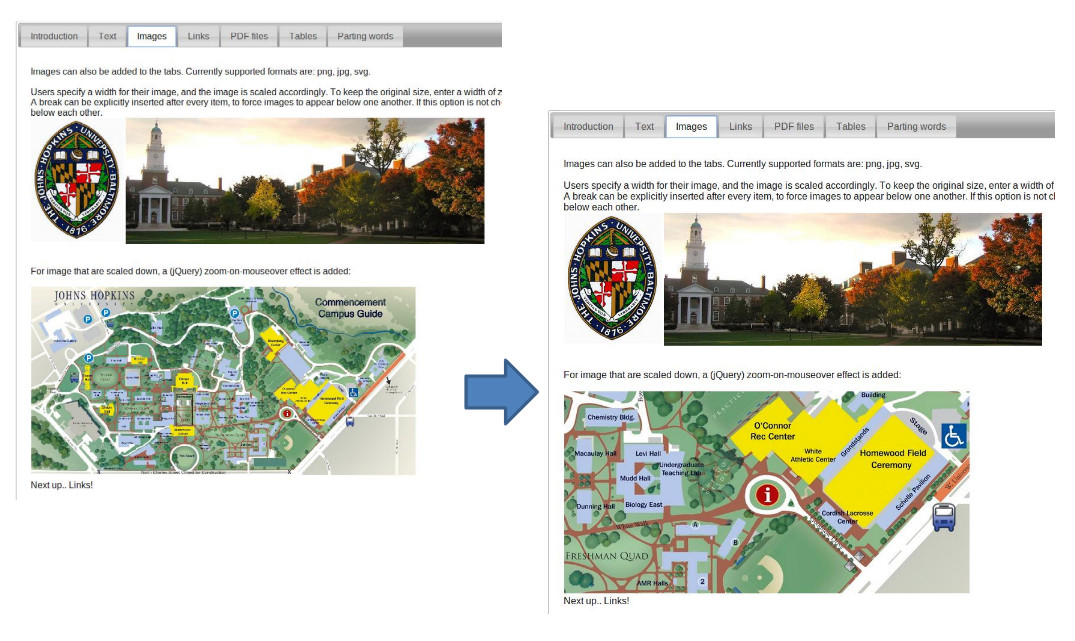
\includegraphics[width=\textwidth]{chapters/images/iReport/Hiltemann_zoomeffect.jpg}
    \caption{Zoom effect.Images that have been scaled down can optionally be enhanced with a jQuery zoom-on-mouseover effect. In this example, the bottom image has this effect added, and when the user moves their mouse over the image, a zoomed version of that area of the image is shown. }
    \label{fig:imagezoom}
\end{figure}

\paragraph*{Content item: Tables}
iReport can also display tables. The input must be a tab-delimited file from the users' Galaxy history, and the first nonempty line not starting with a hash symbol (\verb+#+) is assumed to contain the column headers. The jQuery library \emph{DataTables} \cite{url-datatables} is used to create tables which can be searchable, sortable and paginated, if requested by the user. There is an option to create hyperlinks within the columns of a table by providing a column number, a URL prefix and a URL suffix. This is illustrated in \hyperref[fig:collinks]{Figure \ref*{fig:collinks}}, where the first column contains gene names and by including the GeneCards \cite{genecardspaper,url-genecards} URL prefix \verb+http://www.genecards.org/cgi-bin/carddisp.pl?gene=+. This generates a hyperlink to the corresponding GeneCards entry for every item in the column in the table.

%% weblinks from table columns
\begin{figure}[h!]
    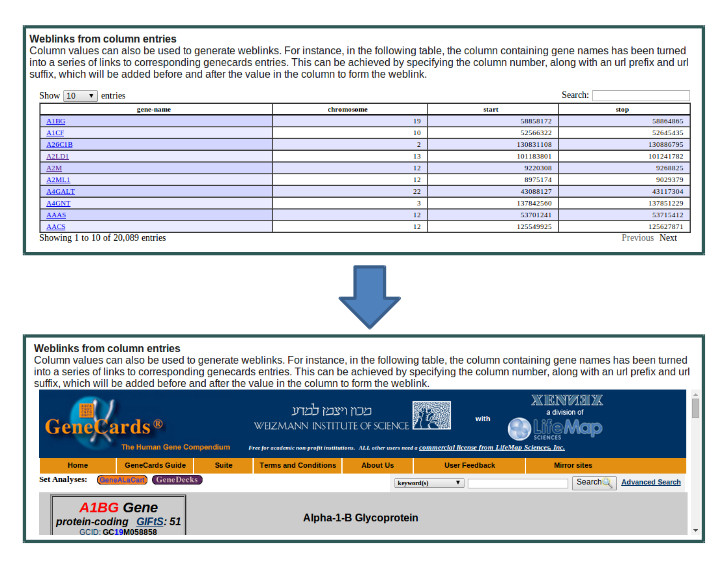
\includegraphics[width=\textwidth]{chapters/images/iReport/Hiltemann_columnlinks.jpg}
    \caption{Weblinks from table columns
   A series of web links can be created within a table by specifying a prefix and suffix to be placed before and after each column entry.}
    \label{fig:collinks}
\end{figure}

\paragraph*{Content item: PDF Files}
This is one of the simplest content items. The user provides a PDF file from the Galaxy history, which will be embedded in the page. If the browser does not have the necessary plug-ins installed, a download link for the file will be generated instead (\hyperref[fig:pdfexample]{Figure \ref*{fig:pdfexample}}).

%% PDF example
\begin{figure}[h!]
    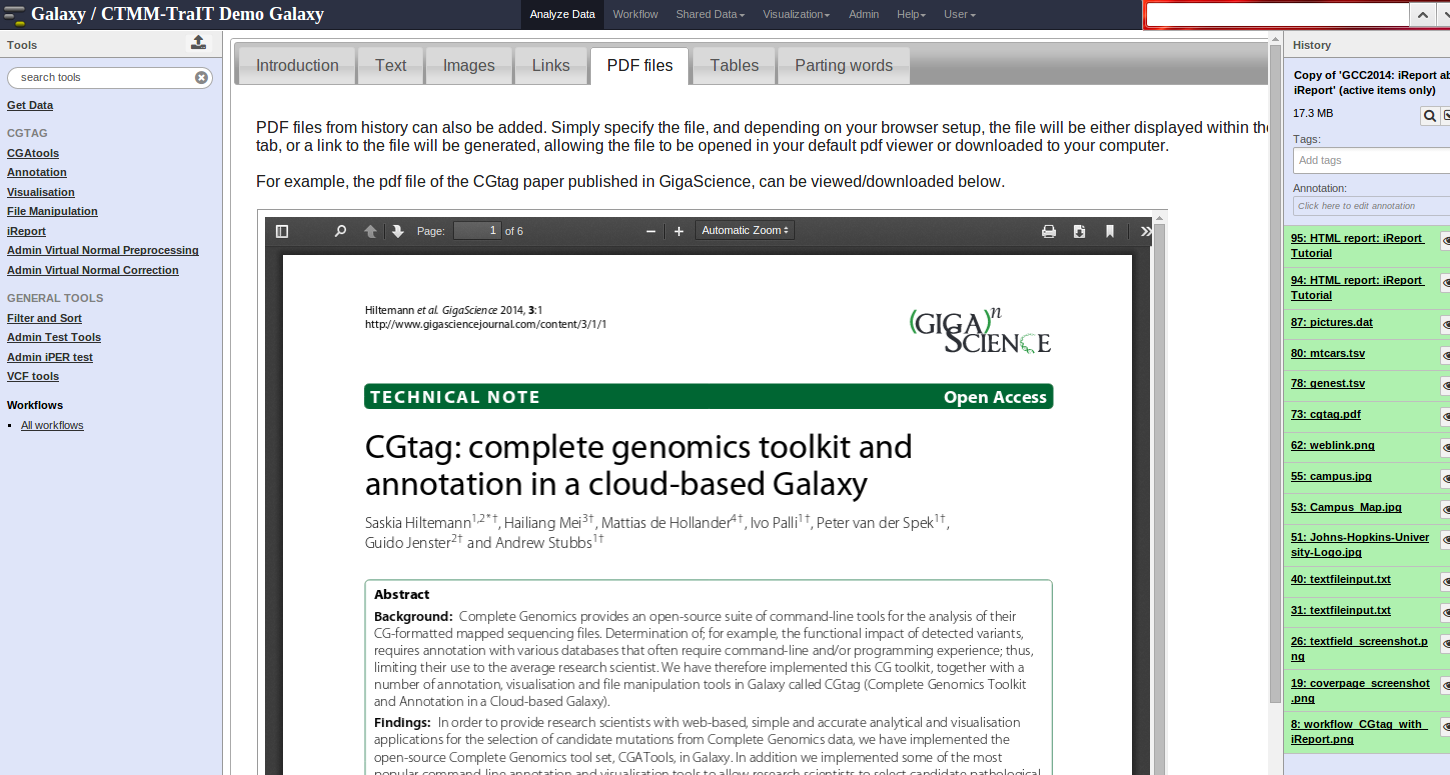
\includegraphics[width=\textwidth]{chapters/images/iReport/Hiltemann_PDF.jpg}
    \caption{Embedded PDF files. iReports can also display PDF files. For browsers without PDF plug-in, a download link to the file will be created instead. }
    \label{fig:pdfexample}
\end{figure}

\paragraph*{Content item: Links}
Users can create links to web locations by specifying a URL and a link text. Links to datasets in the history can also be created here by specifying a dataset and a link text. Several tools create archives of files as output (for example a zip file containing the plots for each chromosome). Links to all files contained in an archive can also be created, and will be named with the file names (excluding file extension). Currently the supported archive formats are zip, bz2, tar, gz and tar.gz. An example can be seen in \hyperref[fig:archivelinks]{Figure \ref*{fig:archivelinks}}, where an archive with images was used as input and a series of links to each contained file was created. An option to create a link to an iReport is also present. This allows users to create a kind of electronic lab notebook, by creating an overview of all their samples and linking to one or more iReports for each sample.

%% links from archive
\begin{figure}[h!]
    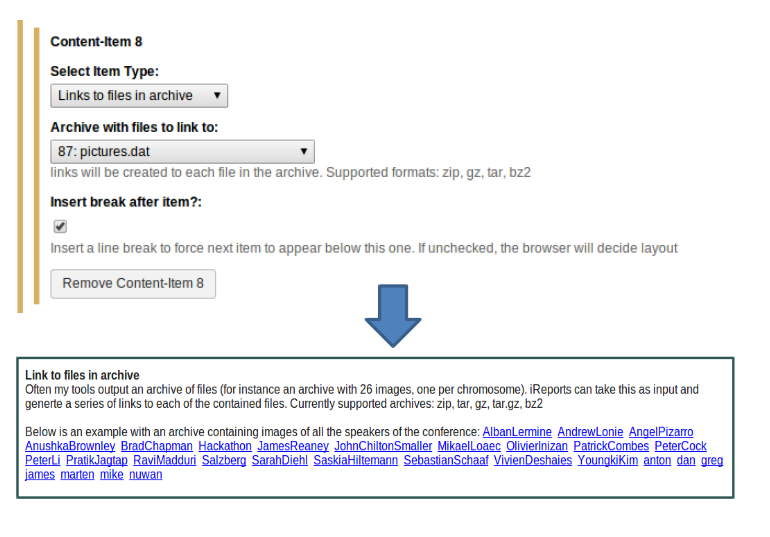
\includegraphics[width=\textwidth]{chapters/images/iReport/Hiltemann_archivelinks.jpg}
    \caption{Links to all files in an archive.Given an archive of files, iReport can create a series of links to all files contained in the archive. Link texts are the filenames (without file extension).}
    \label{fig:archivelinks}
\end{figure}

\section*{Genetic report for a trio of HapMap individuals}

Accurate, reproducible and traceable reporting is an essentialrequirement to the evaluation of the genetic outcome from any assay \cite{skyline}, including those variations predicted from NGS analysis. Since iReport is capable of including many formats, we have used the outcome from a trio analysis generated from the Complete Genomics \cite{drmanac} NGS platform to demonstrate its utility in representing these data in a user-defined format, which contains the provenance of the underlying analysis. In this example we use a trio of individuals sequenced in the International HapMap Project \cite{hapmap}\cite{hapmap2}, to demonstrate how to select protein affecting candidate variants based on a recessive genetic model.  All data in this example is freely available for download from the Complete Genomics website \cite{url-CGpublicdata}.

This example iReport has one tab devoted to explaining the protocol used (\hyperref[fig:trioscreenshots]{Figure \ref*{fig:trioscreenshots}B}), one tab with circos plots and an explanation of the family structure (\hyperref[fig:trioscreenshots]{Figure \ref*{fig:trioscreenshots}D}), and one tab with tables containing the candidate pathogenic variants determined by the protocol based on a recessive model for selection. This iReport is also available as a published history on the TraIT-CTMM public Galaxy \cite{url-traitgalaxy}.

%% Genetic Report
% file: Hiltemann_geneticreport[A-D].jpg
\begin{figure}[h!]
   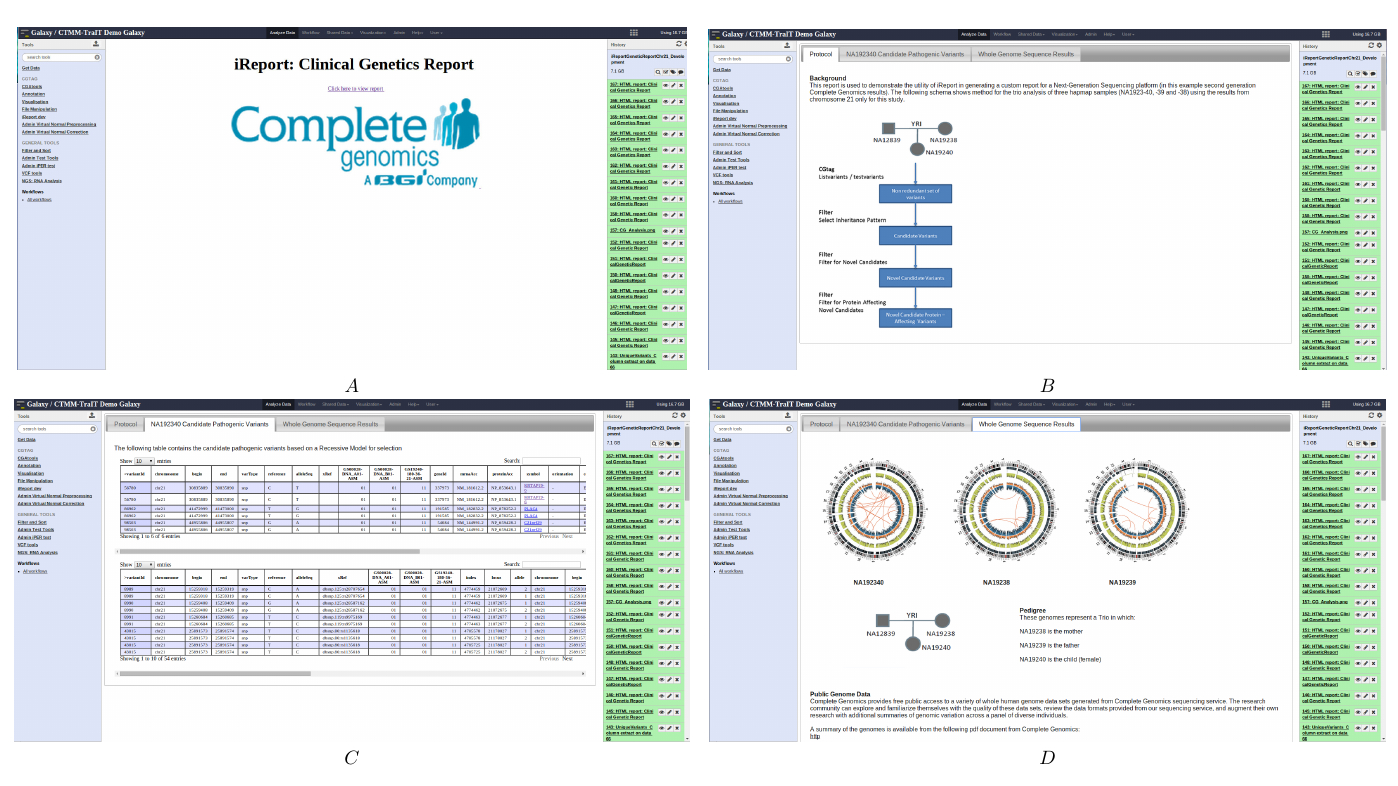
\includegraphics[width=\textwidth]{chapters/images/iReport/Hiltemann_geneticreport.jpg}
%    \begin{center}$
%    \begin{array}{cc}
%    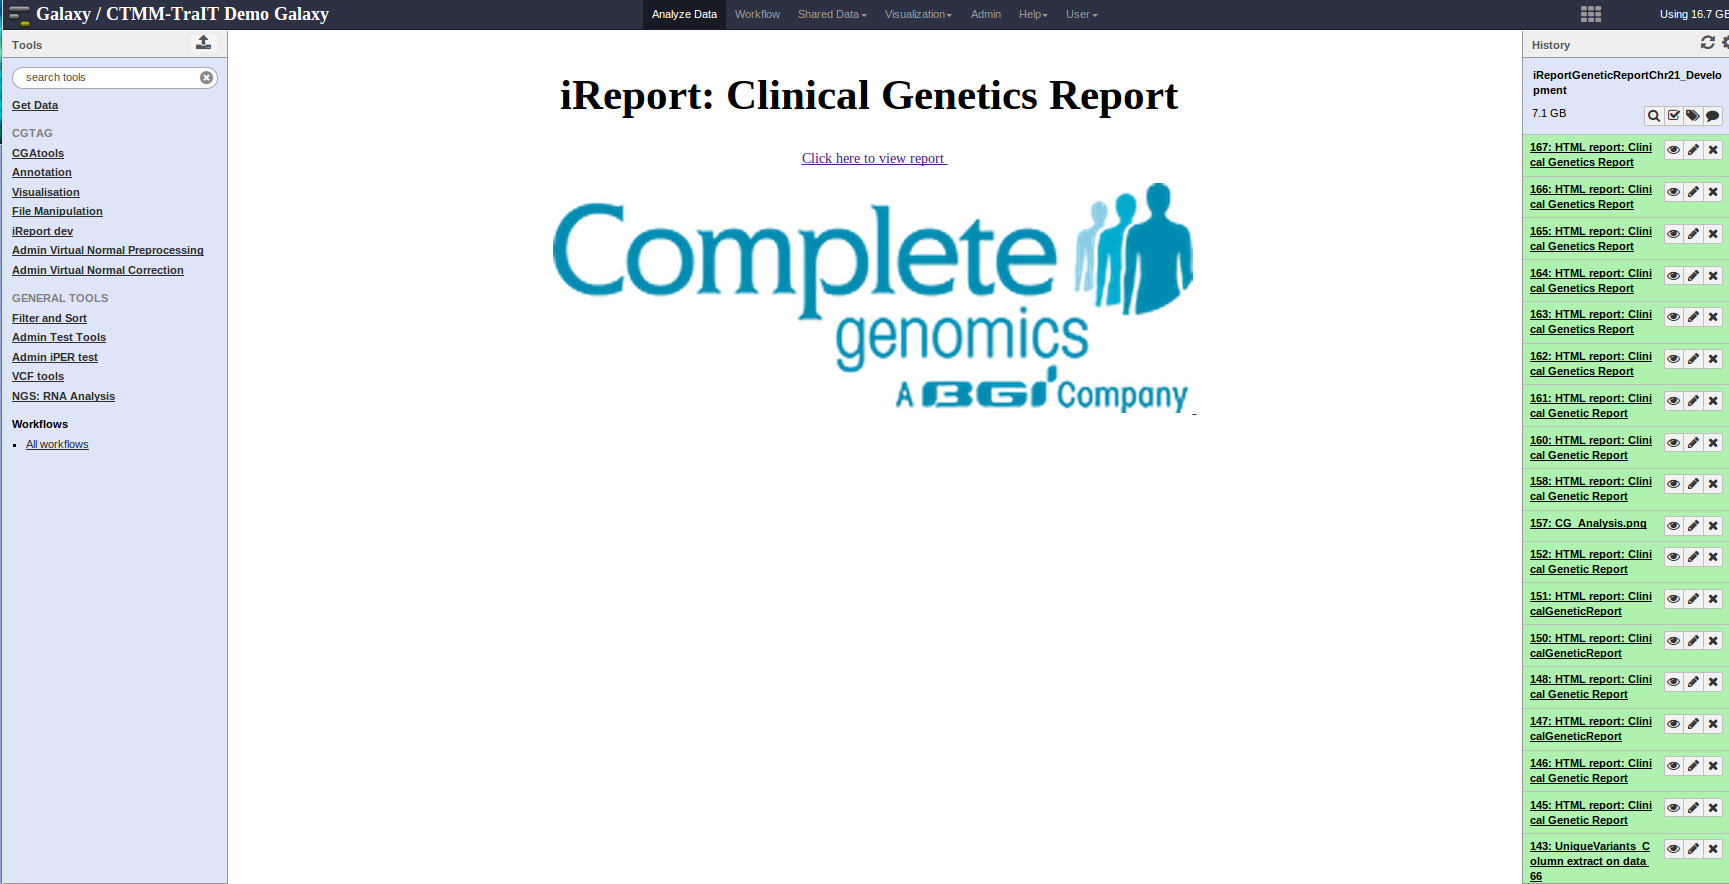
\includegraphics[scale=0.08]{chapters/images/iReport/Hiltemann_geneticreportA.jpg}   &
%    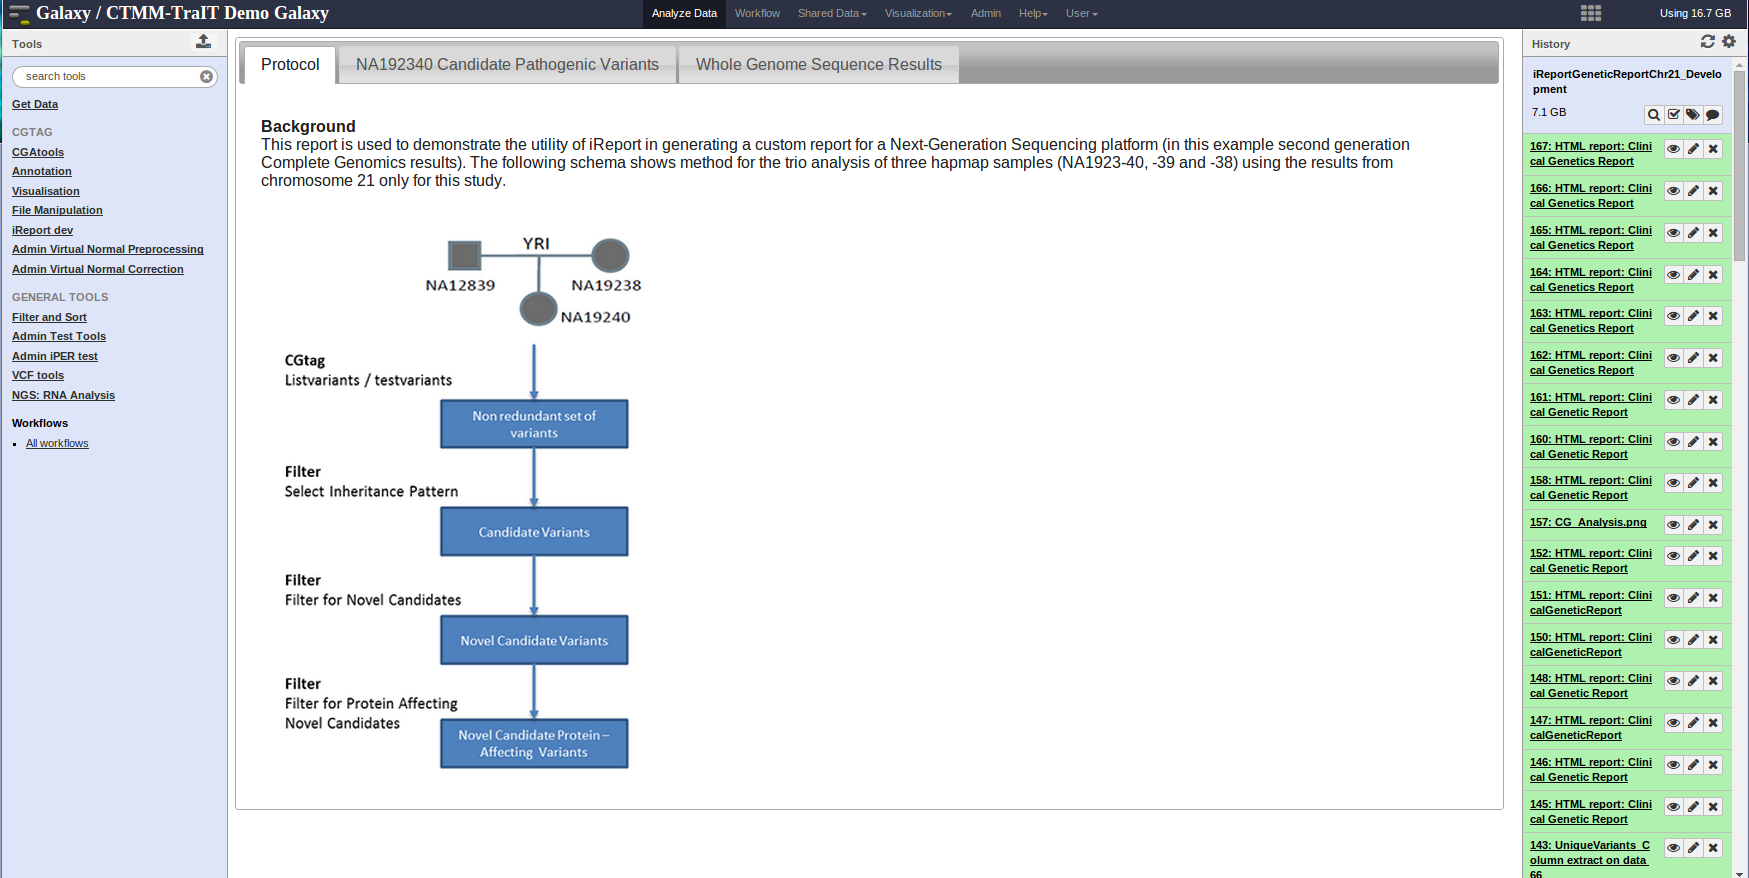
\includegraphics[scale=0.08]{chapters/images/iReport/Hiltemann_geneticreportB.jpg}   \\
%    A & B \\
%    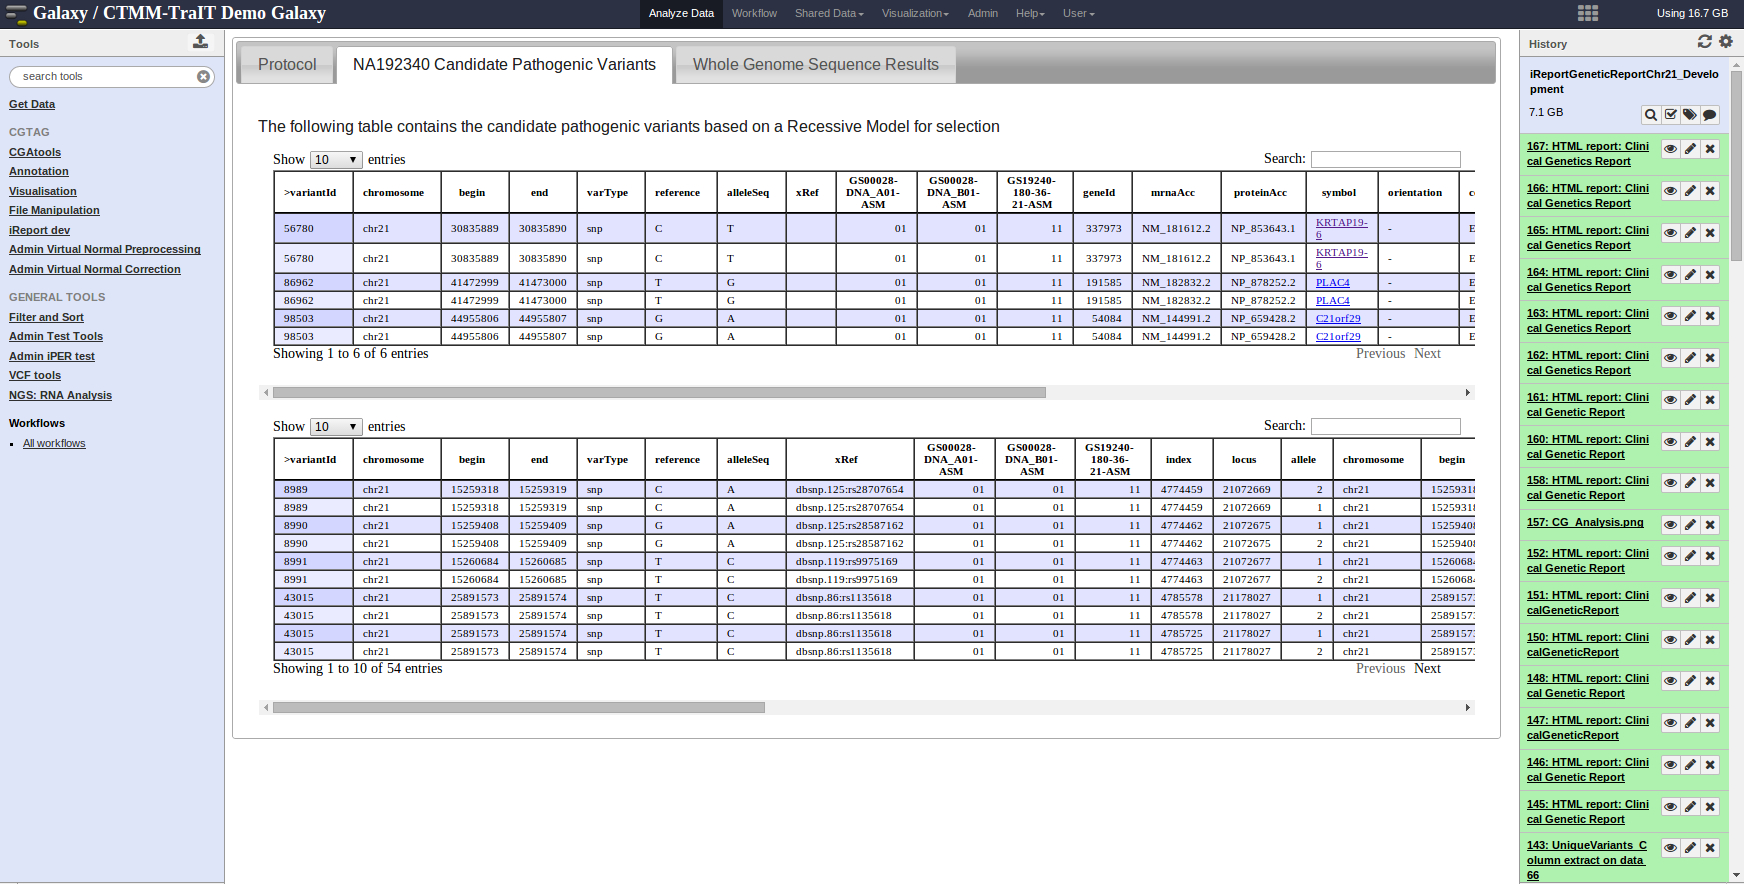
\includegraphics[scale=0.08]{chapters/images/iReport/Hiltemann_geneticreportC.jpg}   &
%    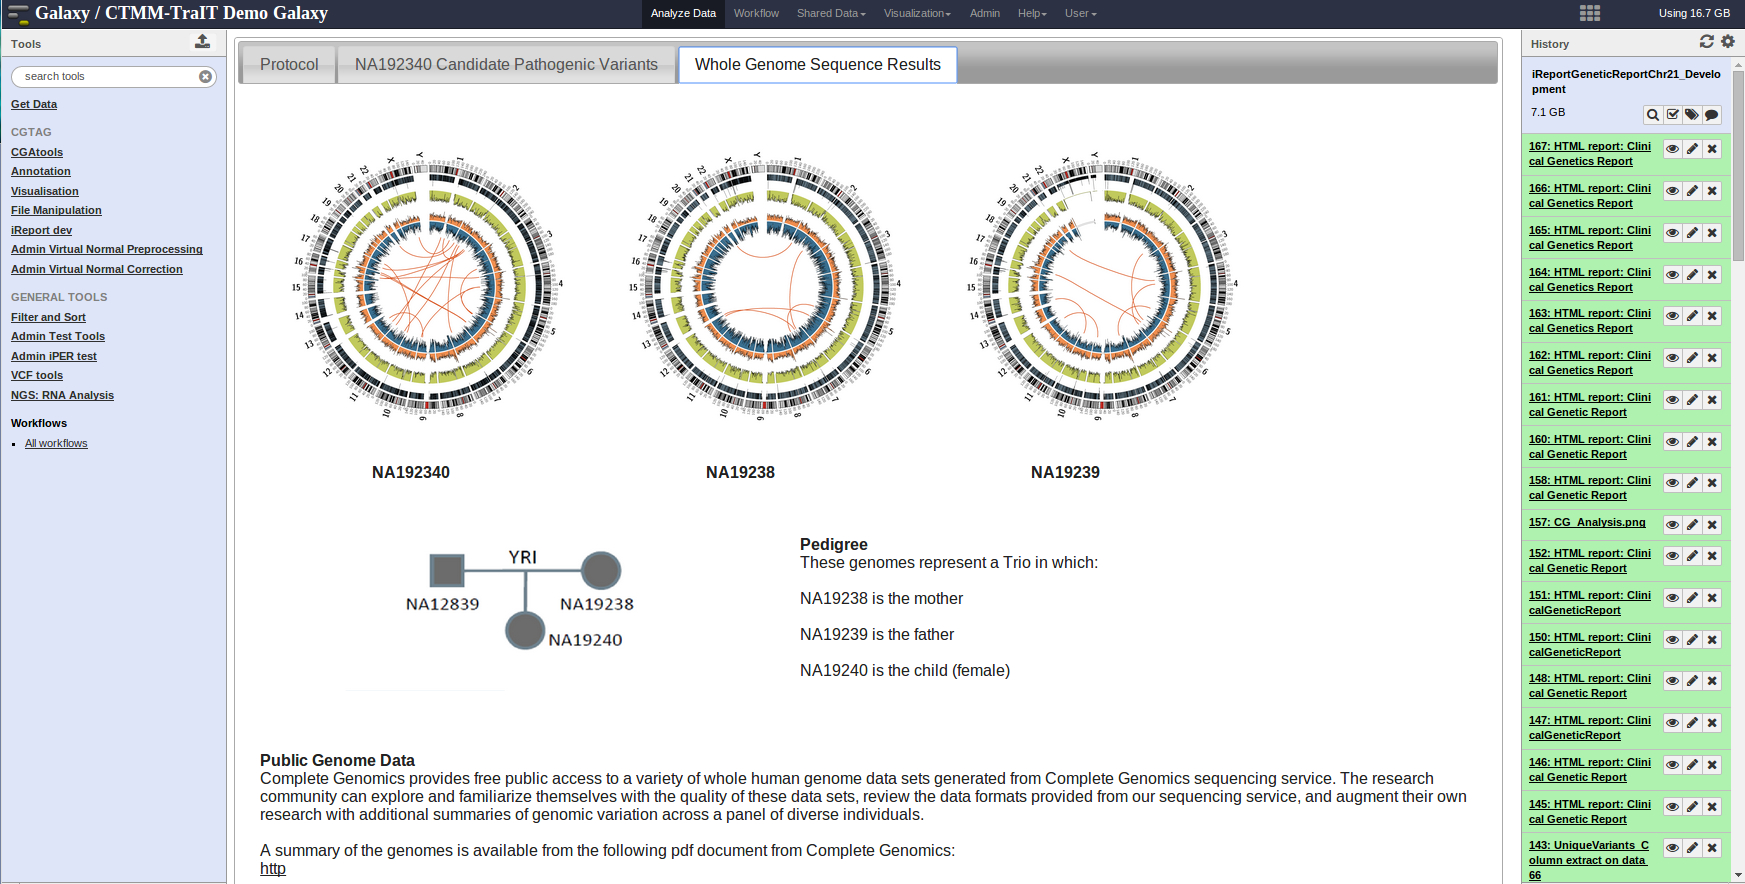
\includegraphics[scale=0.08]{chapters/images/iReport/Hiltemann_geneticreportD.jpg}   \\
%    C & D \\
%    \end{array}$
%    \end{center}
    \caption{Example iReport: Genetic Report. Example iReport for Clinical Genetics. A) Cover page with custom image. B) First tab, explaining the protocol used. C) Second tab, tables of candidate pathogenic variants, gene columns linking out to GeneCards. D) Fourth tab showing Circos images and family structure.  }
    \label{fig:trioscreenshots}
\end{figure}

\section*{Conclusions}
iReport is a easy-to-use, flexible tool for generating traceable, standardized reports which are easily shared between users within and across platforms. We have demonstrated that iReport is capable of creating a customised genetics report from results generated within Galaxy and may be shared with collaborators on the same platform, or with the public. Additionally, data or results generated externally can be uploaded into Galaxy and can also be used by iReport. These reports are generated as web pages and may be downloaded in their entirety to be easily shared across systems.

The genetics report presented here represents the bare minimal reporting that is required to summarise the output for a genetic variation analysis. Whilst we used a trio of individuals to demonstrate how to select protein-affecting candidate variants based on a recessive model, any number of model outcomes and other assay results may be included in an iReport.

We developed iReport to simplify reporting and sharing the output from \emph{omics} and non-high throughput assays analysed both in and external to Galaxy. We have also utilised iReport for more complex analysis workflows, such as summarising translational research and diagnostic applications for cancer and immunological research and diagnostics.

\section*{Availability and requirements}
Project name: iReport \\
Project home page: https://github.com/shiltemann/iReport \\
CTMM-TraIT public Galaxy instance: galaxy.ctmm-trait.nl \\
iReport tool shed repository: https://toolshed.g2.bx.psu.edu/view/saskia-hiltemann/ireport \\
\ \\
Operating system(s): Unix-based Operating Systems \\
Programming languages: Bash, Perl, Python \\
Other Requirements: Galaxy \\
License: GNU GPL \\
Any restrictions to use by non-academics: none \\
\ \\
Examples: \\
iReport about iReport published history: \url{http://galaxy.ctmm-trait.nl/u/saskia-hiltemann/h/gcc2014-ireport-about-ireport}, or \url{tinyurl.com/llrzz9w} \\
Clinical Genetics iReport published history: \url{http://galaxy.ctmm-trait.nl/u/andrew-stubbs/h/ireportgeneticreportchr21} \\

%Tool shed repository for iReport: https://toolshed.g2.bx.psu.edu/view/saskia-hiltemann/ireport \\
%GitHub repository: https://github.com/shiltemann/iReport \\

\section*{Availability and supporting data}
The iReport tool, user manual (published page), and example data and histories are available at the CTMM-TraIT Galaxy server \cite{url-traitgalaxy}.

\section*{Abbreviations}
CGtag: Complete Genomics Toolkit and Annotation in a Cloud-based Galaxy. \\
CTMM-TraIT: Center for Translational Molecular Medicine - Translational IT. \\
NGS: Next Generation Sequencing. \\
URL: Uniform Resource Locator. \\


\section*{Acknowledgements}
 This study was performed within the framework of the Center for Translational Molecular Medicine (CTMM). TraIT project (grant 05T-401).

\bibliographystyle{plain}
\bibliography{references}

\begin{savequote}[75mm]
Nulla facilisi. In vel sem. Morbi id urna in diam dignissim feugiat. Proin molestie tortor eu velit. Aliquam
\qauthor{Quoteauthor Lastname}
\end{savequote}

\chapter{Training}
\label{chapter:training}

Training is a vital component of accessible research. Galaxy enables the domain experts to perform complex analyses without needing to consult with a bioinformatician. This also makes Galaxy an ideal platform for training, allowing learners to focus solely on the analysis and scientific concepts, not the minutia of tool installation and maintenance or the commandline interface details. To this end, we developed a training infrastructure for the Galaxy platform, designed for ease-of-use for both learners and trainers.

\begin{figure}[t!]

\includegraphics[scale=0.1]{chapters/images/training-coverart.jpg}
\end{figure}
\setcounter{figure}{-1}
\setcounter{table}{-1}
\setcounter{section}{-1}

\begin{savequote}[75mm]
This is some random quote to start off the chapter.
\qauthor{Firstname lastname}
\end{savequote}

\chapter{iFUSE \& VCaP Chromothripsis}
\setcounter{figure}{-1}
\setcounter{table}{-1}
\setcounter{section}{-1}

We created iFUSE to explore structural variants and find possible fusion genes, and then used this to detect chromothripsis and multiple fusions in VCaP cell line.

%\includepdf[pages=1-2]{chapters/myarticles/iFUSE.pdf}
\newpage
\articletitle{iFUSE: integrated fusion gene explorer}
Saskia Hiltemann \textsuperscript{1}, Elizabeth A. McClellan\textsuperscript{2}, Jos van Nijnatten\textsuperscript{2}, Sebastiaan Horsman\textsuperscript{2}, Ivo Palli\textsuperscript{2}, Ines Teles Alves\textsuperscript{1,3}, Thomas Hartjes\textsuperscript{1}, Jan Trapman\textsuperscript{3}, Peter van der Spek\textsuperscript{2}, Guido Jenster\textsuperscript{1}, and Andrew Stubbs\textsuperscript{2}

\small
\begin{enumerate}
\itemsep-0.5em
\item Department of Urology, Erasmus MC, 3015 GE Rotterdam, The Netherlands.
\item Department of Bioinformatics, Erasmus MC, 3015 GE Rotterdam, The Netherlands.
\item Department of Pathology, Erasmus MC, 3015 GE Rotterdam, The Netherlands.
\end{enumerate}

Published in: Bioinformatics \\
DOI: \url{10.1093/bioinformatics/btt252} \\

\section*{Abstract}

\textbf{Summary:} We present iFUSE (integrated FUSion gene Explorer), an online visualization tool that provides a fast and informative view of structural variation data and prioritizes those breaks likely representing fusion genes. \color{black} This application uses calculated breakpoints to determine fusion genes based on the latest annotation for genomic sequence information, and where relevant the structural variation (SV) events are annotated with predicted RNA and protein sequences. iFUSE takes as input either a Complete Genomics (CG) junction file, a FusionMap \cite{ge2011fusionmap} fusion detection report file, or a file already analysed and annotated by the iFUSE application on a previous occasion.

\textbf{Results:} We demonstrate the utility of iFUSE with case studies from tumour-normal SV detection derived from Complete Genomics whole-genome sequencing results.

\textbf{Availability:} iFUSE is available as a web service at \url{http://ifuse.erasmusmc.nl}


\section*{Introduction}

Structural variation analysis is a common requirement in the study of cancer where many fusion genes have been implicated in the progression of cancer \cite{mitelman2007impact, kumar2008recurrent}
The use of next-generation sequencing for fusion gene detection in cancer \cite{edgren2011identification, ge2011fusionmap, mcpherson2011defuse}, structural variation in non-cancerous diseases \cite{rareallele, rareallele2} and in normal genomes \cite{1000Genomes} has expanded knowledge of the importance of these events.
In a recent study the use of \textit{de novo} assembly in association with SV detection suggests that SVs account for more diversity between individuals than do single nucleotide polymorphisms (SNPs) \cite{li}. Complete Genomics uses \textit{de novo} assembly during SV, single nucleotide variation (SNV) and copy number variation (CNV) determination \cite{carnevali}.

Traditionally, for a given SV, a user can visualize the individual (sides of the) breaks in viewers such as IGV \cite{igv, igv2}, but not the resulting event or fusion gene as a whole, and must manually retrieve the sequence of the resulting event based on the exons from both genes of the proposed fusion gene and determine the orientation and frame of the predicted transcript and encoded polypeptide sequences. Other applications also offer visualisation, but with the caveat that the user must process their data within the application, e.g inGAP-SV \cite{ingap-sv}, or that a bioinformatician is required to render the visualization using e.g. Circos \cite{circos}. Our aim is to deliver a web-based application that allows scientists to visualize all detected SV events and fusion genes determined in their results and to provide the concomitant candidate transcripts and polypeptide sequences associated with the detected fusion genes (Fig \ref{fig:screenshot}). No other application exists at the moment to categorize and visualize the candidate fusion genes, and determine the proposed sequence for gDNA, RNA and polypeptides from standard SV files.

\begin{figure}
\centerline{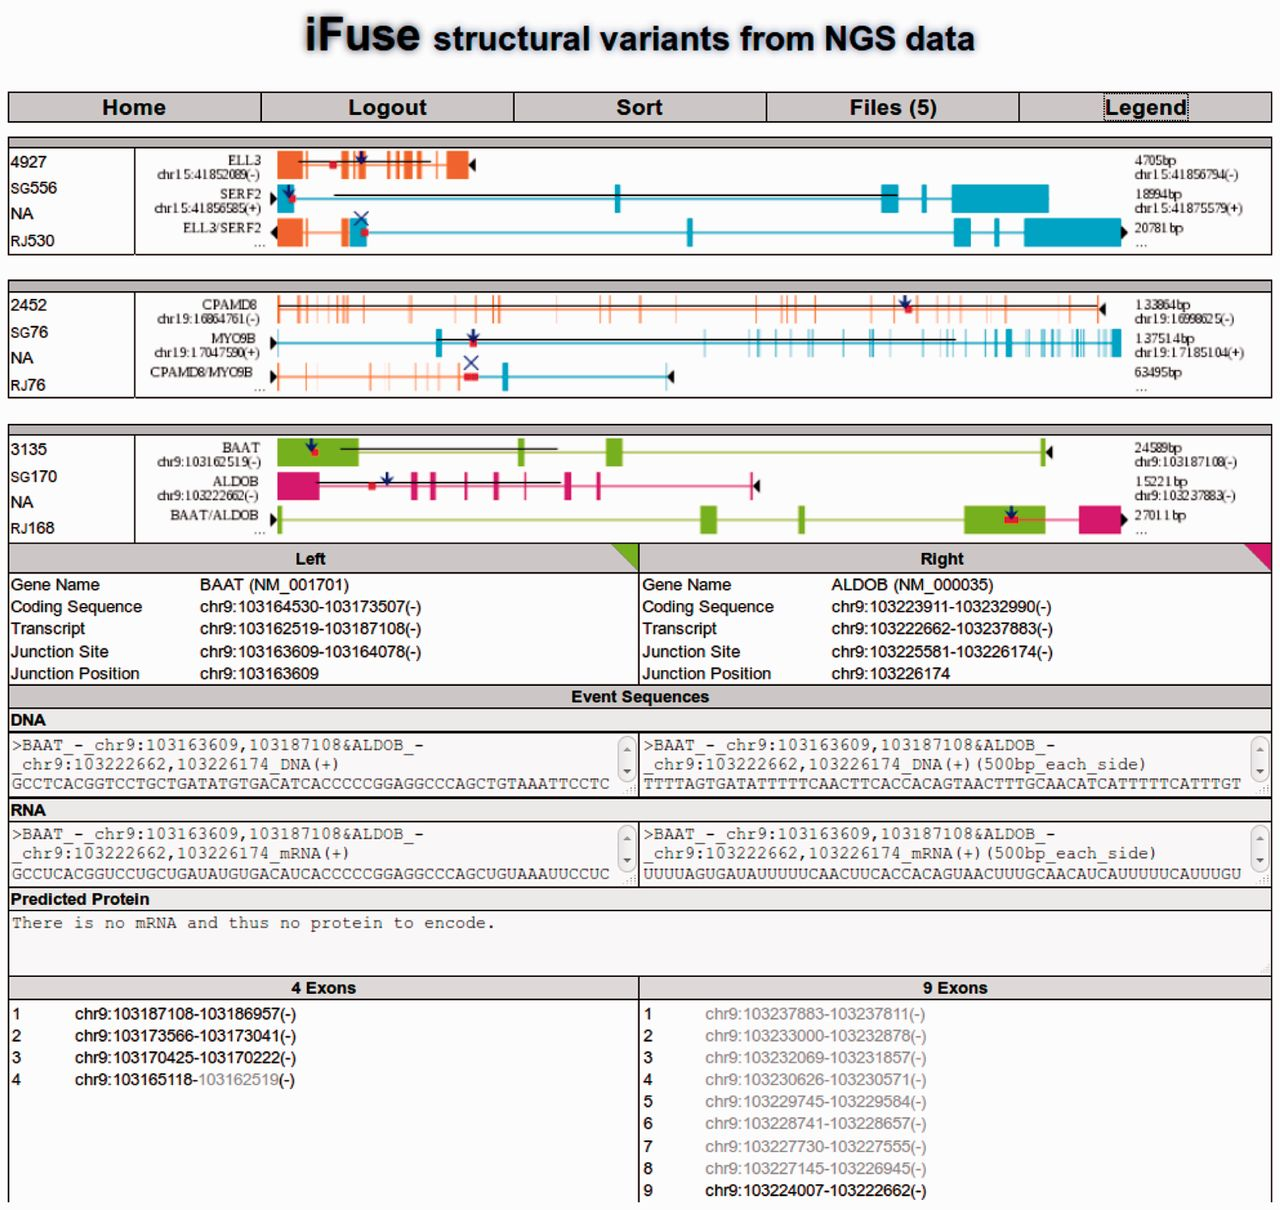
\includegraphics[width=250pt]{chapters/images/iFUSE/ifusess.jpeg}}
\caption{Screenshot of iFUSE. SVs are visualised and where applicable, the predicted DNA, RNA and protein sequences are reported.}
\label{fig:screenshot}
\end{figure}


\section*{Methods}

iFUSE is a PHP-coded application running on an Apache web server with a mySQL database for user management and R for data analysis. Gene-based feature annotation is provided using the UCSC gene tables (hg18 and hg19). Documentation details, including full application configuration, are available from the website (\href{http://ifuse.erasmusmc.nl}{http://ifuse.erasmusmc.nl}).

iFUSE takes as input either a Complete Genomics (CG) junctions file or a fusion detection report as generated by the FusionMap tool \cite{ge2011fusionmap}.  To perform a comparison of two or more genomes, the Complete Genomics tool Junctions2Events can be used prior to visualisation within iFUSE.\color{black}
The input file is validated and then analyzed using R, after which a graphical representation for each event is generated. This representation displays the promotor, introns, exons and the junction site, and additional information including DNA, RNA and protein sequences are presented to the user. These events can be filtered and sorted by the user, either using general properties or by zooming in on a single event and filtering for nearby junctions or events with similar properties.

The input files uploaded to iFUSE are annotated in R using information retrieved from UCSC gene tables and the input files. The resulting output file can be retrieved from iFUSE for manual inspection, and can also be used directly as input to iFUSE.

Example input files can be downloaded from the downloads section of the iFUSE website and users can test the application without registration by selecting the option to start an anonymous session. Any files uploaded by the user will be deleted at the end of the anonymous session.

iFUSE accounts are password protected, the application has been tested for security risks such as SQL injections, and our servers undergo periodical CERT vulnerability scans (http://www.cert.org). Furthermore, when a user deletes a file via the iFUSE web interface, it is purged completely from our systems.

\section*{Discussion}


Two public cancer genomes have been used to demonstrate the utility of iFUSE for the prediction of fusion genes. Genomes were downloaded from Complete Genomics (\href{ftp2.completegenomics.com}{ftp2.completegenomics.com}). The results can be found in Table \ref{tab:results}.


\begin{table}[!t]
    \begin{tabular}{lcccc}
        \toprule
                              & S1 Tumour  & S1 Normal  & S2 Tumour   & S2 Normal \\
        \midrule
        HG18                  &            &            &             &         \\
        Junctions             & 1579       & 1594       & 1558        & 1387    \\
        Genes on both sides   & 32         & 15         & 23          & 4       \\
        Same orientation      & 21         & 14         & 16          & 1       \\
                              &            &            &             &         \\
        HG19                  &            &            &             &         \\
        Junctions             & 1581       & 1592       & 1559        & 1390    \\
        Genes on both sides   & 21         & 12         & 31          & 7       \\
        Same orientation      & 10         & 6          & 17          & 3       \\
        \toprule
    \end{tabular}
    \caption{Results from iFUSE on public datasets. Sample 1 (S1): HCC1187, Sample 2 (S2): HCC2218, public datasets downloadable from Complete Genomics. (ftp://ftp2.completegenomics.com/Cancer\_pairs/)
    }
    \label{tab:results}
\end{table}

An event is labeled as a fusion gene if the breakpoint has two different genes on either side. If the two sides also have the same orientation (are on the same strand, or in the case of an inversion on opposite strands) and are also in frame, the event is called a fusion protein.

\section*{Conclusion}

iFUSE provides scientists with a convenient method to visualize, categorize, and filter structural variation analysis output using Complete Genomics junction files or the FusionMap fusion detection report files as input to the application.

\section*{Acknowledgements}

This study was performed within the framework of CTMM, the Center for Translational Molecular Medicine. TraIT project (grant 05T-401).

We would like to thank Rick Tearle and Steve Lincoln from Complete Genomics whose valuable discussions on Complete Genomics analysis methods supported our application development.


\bibliographystyle{plain}
\bibliography{references}

\begin{savequote}[75mm]
Nulla facilisi. In vel sem. Morbi id urna in diam dignissim feugiat. Proin molestie tortor eu velit. Aliquam erat volutpat. Nullam ultrices, diam tempus vulputate egestas, eros pede varius leo.
\qauthor{Quoteauthor Lastname}
\end{savequote}

\chapter{Somatic Variant Detection}
\setcounter{figure}{-1}
\setcounter{table}{-1}
\setcounter{section}{-1}
\setcounter{NAT@ctr}{-1}

We integrated the Complete Genomics toolsuite into Galaxy and used it to analyse tumour samples without a matching normal.


\newpage
\phantomsection
\addcontentsline{toc}{section}{The Informatics: CGtag}
\articletitle{CGtag: Complete Genomics Toolkit and\\Annotation in a Cloud-based Galaxy}
Saskia Hiltemann\textsuperscript{\ref{affil:emc},*},
Hailiang Mei\textsuperscript{\ref{affil:nbic}},
Mattias de Hollander\textsuperscript{\ref{affil:knaw}},
Ivo Palli\textsuperscript{\ref{affil:emc}},
Peter van der Spek\textsuperscript{\ref{affil:emc}},
Guido Jenster\textsuperscript{\ref{affil:emc-uro}},
Andrew Stubbs\textsuperscript{\ref{affil:knaw}}

\small
\begin{enumerate}
\itemsep-0.5em
\item Department of Bioinformatics, Erasmus Medical Centre, Rotterdam, The Netherlands. \label{affil:emc}
\item Netherlands Bioinformatics Center, NBIC, Nijmegen, The Netherlands \label{affil:nbic}
\item Department of Microbial Ecology, Netherlands Institute of Ecology, NIOO-KNAW, Wageningen, The Netherlands \label{affil:knaw}
\item Department of Urology, Erasmus Medical Centre, Rotterdam,  The Netherlands \label{affil:emc-uro}
\end{enumerate}
\normalsize

Published in: GigaScience, January 2014 \\
DOI: \url{https://doi.org/10.1186/2047-217X-3-1}

\section*{abstract}

\textbf{Background:} Complete Genomics provides an open-source suite of command-line tools for the analysis of their CG-formatted mapped sequencing files. Determination of; for example, the functional impact of detected variants, requires annotation with various databases that often require command-line and/or programming experience; thus, limiting their use to the average research scientist. We have therefore implemented this CG toolkit, together with a number of annotation, visualisation and file manipulation tools in Galaxy called CGtag (Complete Genomics Toolkit and Annotation in a Cloud-based Galaxy).


\textbf{Findings:} In order to provide research scientists with web-based, simple and accurate analytical and visualisation applications for the selection of candidate mutations from Complete Genomics data, we have implemented the open-source Complete Genomics tool set, CGATools, in Galaxy. In addition we implemented some of the most popular command-line annotation and visualisation tools to allow research scientists to select candidate pathological mutations (SNV, and indels). Furthermore, we have developed a cloud-based public Galaxy instance to host the CGtag toolkit and other associated modules.

\textbf{Conclusions:} CGtag provides a user-friendly interface to all research scientists wishing to select candidate variants from CG or other next-generation sequencing platforms’ data. By using a cloud-based infrastructure, we can also assure sufficient and on-demand computation and storage resources to handle the analysis tasks. The tools are freely available for use from an NBIC/CTMM-TraIT (The Netherlands Bioinformatics Center/Center for Translational Molecular Medicine) cloud-based Galaxy instance, or can be installed to a local (production) Galaxy via the NBIC Galaxy tool shed.

\textbf{Keywords:} Complete Genomics, Next Generation Sequencing, Genetic variation, Pathogenic gene selection.



\section*{Findings }

\subsection*{Background}

Complete Genomics (CG) supplies results for whole-genome next-generation sequencing (NGS) data mapped to a user-defined genome \cite{ma} and additional open-source tools \cite{url-cgatools} for further characterisation of the sequenced genomes. Whilst these tools are open-source and available for download and use on the command-line, they are not amenable for scientists to use from their desktop, and require scripting skills to link these tools together with other applications to successfully prioritise candidate pathogenic genes based on these NGS results. To address this issue, we implemented the Complete Genomics Analysis Toolkit (CGATools), including several functional annotation and visualisation tools in a cloud-enabled instance of Galaxy. Galaxy offers a web-based graphical user interface to command-line tools, and allows for the graphical construction of complex workflows; Galaxy will automatically keep track of the analysis history, and allows for easy sharing and publishing of data and/or workflows with other users \cite{goecks2010galaxy, blankenberg2010galaxy2, giardine2005galaxy}. Furthermore, Galaxy is an extensible platform, nearly any software tool may be integrated into Galaxy, and there is an active community of users and developers ensuring the latest tools are made available for use in Galaxy through the Galaxy tool shed.

This implementation of the CGATools in a Galaxy environment simplifies the analysis of genomes via the Galaxy GUI and the cloud resource ensures that sufficient computing power is available for the analysis. The inherent functionality in Galaxy of CGtag enables the creation of customisable user-defined workflows by the scientist and not only by the bioinformatician.

For large datasets, transfer to Galaxy via SFTP is available and recommended, but is still limited by the upload speed of the user’s internet connection, and can be a bottleneck in the analysis of large datasets.


\subsection*{Variant Detection}

CGATools is an open-source project to provide tools for downstream analysis of Complete Genomics data, and may be downloaded from their repository \cite{url-cgatools}. These tools must be run from the command-line and are therefore, not accessible to all users. To remedy this, Complete Genomics also provide Galaxy tool wrappers for many of the CGAtools, which can be downloaded from the Main Galaxy tool repository (tool shed) \cite{url-toolshed}. However, these Galaxy tools still need to be installed on the users’ local (production) Galaxy instance before they can be utilised. We have now made these tools available on a public server \cite{url-nbicgalaxy}, and have added Galaxy wrappers for those CGAtools that were not provided by Complete Genomics e.g. Junctions2Events, makeVCF (\hyperref[table:tools]{Table \ref{table:tools}}). The use of the CGAtools in \hyperref[table:tools]{Table \ref{table:tools}} have previously been outlined \cite{nieminen}, using a combination of ListVariants and TestVariants or CallDiff to determine candidate pathogenic single nucleotide variants (SNVs), indels and subs in a selected genome as compared with on or more reference genomes or as part of a trio based genetic analysis \cite{nieminen}. The VarFilter may be used to select those variants which have a high confidence based on the underlying sequence reads as specified as VQHIGH, and the SNPDiff tool can then be used to determine concordance of the NGS results with those of an orthogonal SNV detection platform such as an Affymetrix or Illumina SNP array. The JunctionDiff and Junction2Events tools are used to select fusion events and candidate fusion genes based on quality of the discordant reads used to detect the structural variation event \cite{ifuse}.


\begin{table}[t!]
\small
\begin{tabular}{l|l|l}
\textbf{Function} & \textbf{CGATool}  & \textbf{Description} \\ \hline
Variant detection & CGATools ListVariants & Lists the non-redundant set of small variations found in an \\
                  &                       & arbitrary number of genomes.\\
Variant detection & CGATools TestVariants & Determine which variants are found in which genomes given \\
                  &                       & the results of ListVariants.\\
Variant detection & CGATools CallDiff     & Compares two variant files to determine where and how the \\
                  &                       & genomes differ.\\
Variant detection & CGATools VarFilter    & Copies the input varfile or masterVar file, applying filters.\\
Variant detection & CGATools JunctionDiff & Reports difference between junction calls of CG junction files.\\
Variant detection & CGATools Junctions2Events & Groups and annotate related junctions.\\
Quality control   & CGATools SNPDiff      & Compares genotype calls to CG variant files.\\
File merge        & CGATools Join         & Merge two tab-delimited files based on equal field or overlapping \\
                  &                       & regions.\\
Sequence retrieval& CGATools DecodeCRR    & Retrieve sequences from a CRR file for a given range of a \\
                  &                       & chromosome.\\
File conversion   & CGATools mkVCF        & Converts CG variant and/or junction files to VCF.\\
File conversion   & CGATools generateMasterVar & Converts a varfile to a on-line-per-locus format.\\
File conversion   & CGATools fasta-2-crr  & Converts fasta sequences into a single reference crr file.\\
File conversion   & CGATools crr-2-fasta  & Converts crr file to fasta sequence.\\
File conversion   & TestVariants2VCF      & CG community tool. Converts output of the TestVariants tool \\
                  &                       & to VCF.\\
Annotation        & ANNOVAR               & Functional annotation of genetic variants from high-throughput \\
                  &                       & sequencing data.\\
Annotation        & MutationAssessor      & Functional impact of protein mutations.\\
Annotation        & Condel                & CONsensus DELeteriousness score of missense SNVs.\\
Visualisation     & CG Circos plots       & Create CG-style tumour, normal and somatic plots.\\
Visualisation     & Integrative plot      & Create circos plot from CG and SNParray data.\\
Visualisation     & Generic genomic data plotter & Plot any type of numerical genomic data using GNUplot.\\
File manipulation & Filter columns        & Filter tab-delimited files based on column contents.\\
File manipulation & Add/remove chr prefix & adds or removes chr prefix from chromosome column.\\
File manipulation & Column select         & Extract and/or rearrange columns in tab-delimited file.\\
File manipulation & Sort chromosomal position & Sort a tab-delimited file by chromosomal position.\\
File manipulation & Strip header          & Remove header from files.\\
File manipulation & File concatenation    & Concatenate 2 files (e.g. for restoring header).\\

\end{tabular}
\caption{Overview of CGTag tools available in NBIC/CTMM-TraIT Galaxy and the NBIC tool shed}
\label{table:tools}
\end{table}
\normalsize


\subsection*{Functional Annotation Tools}

To provide users with enhanced filtering capabilities, we have integrated several command-line annotation tools in this NBIC/CTMM-TraIT Galaxy instance. ANNOVAR \cite{annovar} is a command-line tool used to functionally annotate genetic variants. We provide a Galaxy tool wrapper for ANNOVAR. This tool will take a list of variants as input and provide gene and amino acid change annotation, SIFT scores, PolyPhen scores, LRT scores, MutationTaster scores, PhyloP conservation scores, GERP++ conservation scores, DGV variant annotation, dbSNP identifiers, 1000 Genomes Project allele frequencies, NHLBI-ESP 6500 exome project allele frequencies, and other information. We have implemented this tool to accept VCF (v4) files, Complete Genomics varfiles or CG-derived tab-separated files using the CG 0-based half-open coordinate system, or lastly, the standard ANNOVAR input format consisting of tab-separated lists of variants using the 1-based coordinate system. This tool will output the original file columns, followed by additional ANNOVAR columns. The ANNOVAR code itself is not included in the tool shed repository, but instructions on how to obtain a license and the subsequent manual installation of the tool are included in the readme of the Galaxy tool shed repository. We obtained permission to offer ANNOVAR on our public Galaxy server, so the tool can be previewed there. To supplement ANNOVAR, Condel (CONsensus DELeteriousness) \cite{condel} has been included to calculate the deleterious score associated of missense SNVs and the impact of non-synonymous SNVs on protein function. Condel integrates the outputs of two tools: SIFT and Polyphen2, to calculate a weighted average of the scores (WAS) of these tools. Condel can optionally incorporate the output of a third tool, MutationAssessor, which is also included in this Galaxy instance. Mutation Assessor \cite{mutass} is a web-based tool providing predictions of the functional impact of amino-acid substitutions in proteins, such as mutations discovered in cancer or missense polymorphisms. The MutationAssessor database is accessed through a REST API. In order not to overload the server, queries are limited to 3 per second, so when dealing with a long list of variants, some pre-filtering is recommended. The functional annotation provided by ANNOVAR, including the addition of multiple versions of dbSNP, the variants provided by Complete Genomics Public data from unrelated individuals only \cite{url-cgftp} and 31 genomes from Huvariome \cite{huvariome}, are available in this Galaxy instance. Huvariome provides the user with additional whole genome variant calls for those regions which are difficult to sequence and can retrieve the weighted allele frequency for each base in the human genome \cite{huvariome}.



\subsection*{Visualisation Tools}

\begin{figure}[t!]
\centering
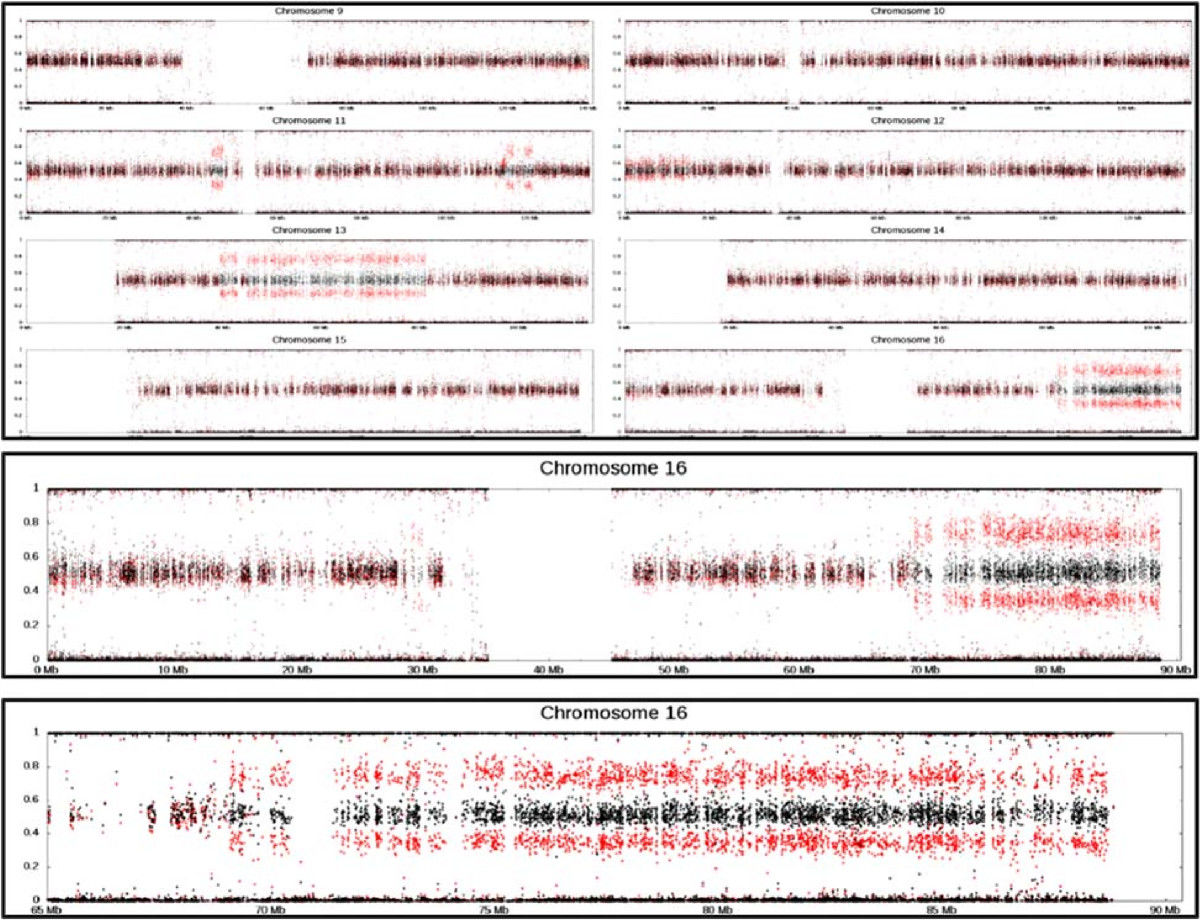
\includegraphics[scale=1.5]{chapters/images/cgtag/fig1-plotter.png}
\caption{\textbf{Generic Genomic data plotting tool.} Output from our generic genomic data plotter used to plot B-allele frequency from Illumina 1M SNParray data. Plot with two tracks; tumour (red) and normal (black). Output can be (top) a whole genome overview (shown here in part), or (middle) a single chromosome, or (bottom) a subregion of a chromosome defined by the user (here chr16, 60MB-end). Many parameters such as the colour and sizes of the data points may be adjusted by the user as required.}
\label{fig:plotter}
\end{figure}


A generic genomic data plotter tool based on GNUplot is available, which takes as input, a tab-delimited file of format chr–start-end–value, and will output either a single chromosome plot, an overview of all chromosome plots in a single image, or a sub-region of a chromosome defined by the user. Additionally, the tool has the option of plotting input from a second file in the same image, which is useful for tumour-normal comparison (\hyperref[fig:plotter]{Figure \ref{fig:plotter}}). B-allele frequency (BAF) is used to determine whether the structural variation junction is homo- or heterozygous. When the data is in the right format, the generic plotter tool can be used to visualise the BAF, and we have also implemented a plot tool to display allele frequencies directly from a CG masterVar file, again with the capability of displaying single-chromosome plots, all chromosomes in a single image, or custom defined regions (\hyperref[fig:plotter]{Figure \ref{fig:plotter}}). The current Complete Genomics analysis pipeline (CGAP v2.5) delivers Circos \cite{url-circos} visualisations with each genome that is sequenced and the code used to generate these images have been made freely available for download \cite{url-cgcircos}. We have modified this code and implemented Galaxy tools to allow for the generation of these images for samples sequenced on earlier CG analysis pipelines (before v2.0), that utilise the junctions file, masterVar file, CNV details and CNV segments files to generate the standard CG Circos report.


To support fusion gene analysis we have created a custom Circos tool which uses CG files, CG junctions file and CG varfile for NGS, and the results from SNP arrays analysis, specifically the B-allele frequency (BAF) and copy number variation (CNV) files. The output is either a whole-genome plot, per-chromosome plots, a single image containing all the per-chromosome plots together, or a plot of a custom region defined by the user (e.g., a plot showing just chromosomes 3, 5, and X, or a plot showing a specific range within a single chromosome). Additionally the user can select an “impacted genes” track for the per-chromosome plots, which will print the names of the genes impacted by SV events along the outer edge of the image (\hyperref[fig:circos]{Figure \ref{fig:circos}}). This custom Circos script is capable of using fusion gene detection results generated from the Illumina platform with the fusion genes detected by an application such as FusionMap \cite{ge2011fusionmap}, and which are reported in custom FusionMap report format, a tab-delimited file similar to that delivered by Complete Genomics.


\begin{figure}[t!]
\centering
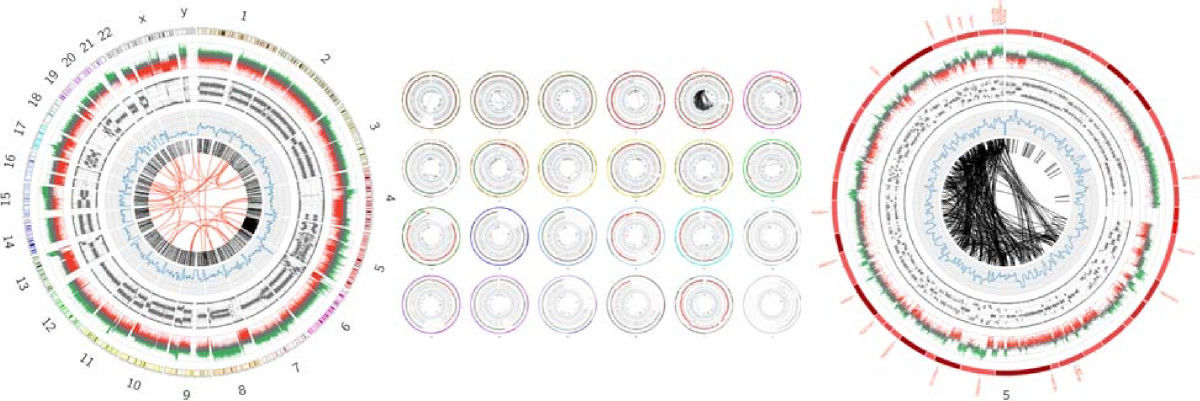
\includegraphics[scale=2]{chapters/images/cgtag/fig2-circos.png}
\caption{\textbf{Circos Integrative Plot Tool.} Circos plots for (left) whole genome, (middle) overview or all chromosomes in single images, and (right) for a single chromosome.  Each chromosome is represented in the outer ring and then from outer to inner rings represent copy number variation (with regions of gain depicted in green and loss in red), B-allele frequency, SNP density and the intra- and interchromosomal rearrangements are on the inside and depicted in black and red lines, respectively.  Impacted genes track (red gene symbols) are displayed outside the outer chromosome ring and only on the single chromosome plot.}
\label{fig:circos}
\end{figure}


In addition to these tools within Galaxy, structural variation files processed using CGtag may be exported to our previously described fusion gene prioritisation tool, iFUSE \cite{url-ifuse} to identify candidate fusion genes and display their representative DNA, RNA and protein sequence.


\subsection*{Auxiliary Tools}

Our suite of tools also includes several auxiliary tools supplied by CG but not available from the Galaxy tool shed which offer the user several file format conversion tools (\hyperref[table:tools]{Table \ref{table:tools}}) that enable users to connect the output from the CGATools analysis to other analytical or annotation workflows by means of standard file formats (e.g., FASTA, VCF). In addition a number of file formatting tools are also included, such as removing of headers from files (required by some tools), adding removing of a chr prefix to a column of a file (i.e., chrX vs. X), concatenation of files, and extracting and rearranging of columns, to help facilitate the flow of data from one tool to the next.

\subsection*{CLOUD Implementation}

NBIC Galaxy is hosted at a high performance computing (HPC) cloud system operated by SURFsara \cite{url-surfsara}. This HPC cloud consists of 19 fast servers with 608 CPUs and almost 5TB of memory. The NBIC Galaxy that operates in this HPC cloud is implemented using the Cloudman framework \cite{afgan} and its adapted version supports the OpenNebula Cloud environment. The advantage of using the Cloudman framework to build NBIC Galaxy is mainly two-fold, firstly Cloudman provides a set of complete scripts to automatically install tools and datasets on a virtual machine image. The installed tools include the Galaxy system itself and all its dependencies. These dependencies include webserver (nginx), database (postgres), cluster job scheduler (SGE), and common NGS tools, such as bowtie, BWA, samtools, and so forth. The installed datasets include most of the common reference genomes (hg18, hg19, mm9, etc) and their tool-specific index files. Thus, the end product of running Cloudman installation script is a fully functional NBIC Galaxy system operating in the HPC Cloud.

The second contribution of Cloudman to our NBIC Galaxy system is its ability to set up a flexible virtual cluster and ability to provide auto-scaling support. The previous NBIC Galaxy was hosted on a dedicate physical server with rather limit resources (4 CPU, 32G memory). Due to this resource limitation, our NBIC Galaxy was never promoted to be a real data analysis server to handle the production level of NGS datasets. On the other hand, because of the sporadic nature of user access, the server was mostly on idle during its 2-year lifespan. Moving to Cloud resolved both issues. The current NBIC Galaxy operates on top of a virtual cluster. This virtual cluster contains one head node and a number of worker nodes. These nodes are all virtual machines that are built using the machine image generated by the Cloudman script. During minimal usage, the cluster will only contain one head node. Once a significant load occurs due to training courses or production level data analysis, the virtual cluster can automatically scale itself upwards. More worker nodes will be added dynamically to this virtual cluster to boost the capacity of NBIC Galaxy. Once the load decreases, the virtual cluster can scale down again to operate with only a limited number of nodes.

The use of shared resources does have drawback as well. We have experienced a more obvious I/O bottleneck in the cloud-based NBIC Galaxy compared to the previous system that ran in a physical machine. In the HPC Cloud, storage is provided through a network file system (NFS) instead of a local hard disk. When more concurrent Cloud users are using the Cloud resource, we observe the extra job time caused by I/O delays. However, we argue that this issue is far outweighed by the benefit of having a dynamic virtual cluster support to the NBIC Galaxy.


\section*{Availability and requirments}

\textbf{Project Name:} CGtag: Complete Genomics Toolkit and Annotation in a Cloud-based Galaxy\\
\textbf{Project home page:} http://galaxy-demo.trait-ctmm.cloudlet.sara.nl\\
\textbf{Operating system:} Linux (Galaxy and CGtag)\\
\textbf{Programming language:} Python (Galaxy and CGtag), R (CGtag), Bash (CGTag) \\
\textbf{Other requirements:} Circos \cite{url-circos}, GNUplot \cite{url-gnuplot}, Complete Genomics open source Toolset \cite{url-cgatools}  and dependencies therein);  see documentation for a comprehensive list of optional dependencies, based on workflow requirements.\\
\textbf{License:} GPL v3\\
\textbf{Any restrictions to use by non-academics:} ANNOVAR license must be obtained before it can be used\\
published page: http://galaxy.ctmm-trait.nl/u/saskia-hiltemann/p/cgtag \\
\textbf{Links to tool shed repositories:}\\
annovar: \url{http://toolshed.nbic.nl/view/saskia-hiltemann/annovar} \\
cgatools: \url{http://toolshed.nbic.nl/view/saskia-hiltemann/cgatools\_v17} \\
circos plotters: \url{http://toolshed.nbic.nl/view/saskia-hiltemann/cg\_circos\_plots} \\
condel: \url{http://toolshed.nbic.nl/view/saskia-hiltemann/condel} \\
file manipulation tools: \url{http://toolshed.nbic.nl/view/saskia-hiltemann/file\_manipulation} \\
generic genomic data plotter: \url{http://toolshed.nbic.nl/view/saskia-hiltemann/genomic\_data\_plotter} \\
mutation assessor: \url{http://toolshed.nbic.nl/view/saskia-hiltemann/mutation\_assessor}\\
NOTE: these tools can be installed to both Cloudman Galaxy instances or non-Cloudman Galaxy instances alike (via the tool shed or manually from the command line).

\section*{Availability and supporting data}

All tools described, as well as example data, are available from the NBIC/CTMM-TraIT Galaxy server (\url{http://galaxy.ctmm-trait.nl}) and the NBIC Galaxy tool shed (\url{http://toolshed.nbic.nl}).

\section*{Notes}

Saskia Hiltemann, Hailiang Mei, Mattias de Hollander, Ivo Palli, Peter van der Spek, Guido Jenster and Andrew Stubbs contributed equally to this work.

\section*{Abbreviations}

\textbf{BAF:} B-allele Frequency \\
\textbf{CG:} Complete Genomics \\
\textbf{CGATools:} Complete Genomics analysis tools \\
\textbf{CGtag:} Complete Genomics Toolkit and Annotation in a Cloud-based Galaxy\\
\textbf{NBIC:} The Netherlands Bioinformatics Center\\
\textbf{NFS:} Network File System \\
\textbf{SNV:} Single Nucleotide Variation\\
\textbf{SV:} Structural Variation\\


\section*{Declarations}

\subsection*{Acknowledgements}

This study was performed within the framework of CTMM, the Center for Translational Molecular Medicine. TraIT project (grant 05T-401).

This work was sponsored by the BiG Grid project for the use of the computing and storage facilities, with financial support from the Netherlandse Organisatie voor Wetenschappelijk Onderzoek (Netherlands Organisation for Scientific Research, NWO)

\subsection*{Note from the Editors}
This paper is part of the GigaScience Galaxy series. We will be hosting some of the computational resources of these papers on our GigaGalaxy server (http://galaxy.cbiit.cuhk.edu.hk).

\subsection*{Competing interests}

The authors declare that they have no competing interests.


\subsection*{Authors contributions}

H, GJ, HM and AS contributed to the design and coordination of CGtag and manuscript preparation. SH, MdH, IP and HM contributed to implementing CGtag.  SH, GJ, PvdS and AS contributed to testing of CGtag. MdH and HM implemented Galaxy Cloudman for the SURFsara/Big-grid HPC cloud. All authors read and approved the final manuscript.


\bibliographystyle{ieeetr}
\bibliography{references}

\begin{savequote}[75mm]
``Humans are allergic to change. They love to say, `We've always done it this way.'' I try to fight that. That's why I have a clock on my wall that runs counter-clockwise.''
\qauthor{Grace Hopper}
\end{savequote}

\chapter{Discussion}\label{discussion}
\setcounter{figure}{-1}
\setcounter{table}{-1}
\setcounter{section}{-1}
\setcounter{NAT@ctr}{-1}

Since the completion of the human reference genome in 2003, the field of molecular biology has been transformed almost beyond recognition, and along with it, the field of bioinformatics has evolved from a niche discipline to an integral part of every biomolecular research question. Where mere decades ago most genomic data analyses could largely be performed by hand, nowadays they often require a supercomputer. Programming knowledge is required to run such analyses, but biologists are not typically trained in these skills, and have thus become reliant on bioinformaticians to carry out this work for them. Similarly, bioinformaticians often lack the increasingly complex biological knowledge required to fully interpret the results~\cite{preeyanon2014reproducible}. Biologist and bioinformatician must therefore work together closely, and each should be trained in the other discipline in order gain awareness of factors that might influence analysis or result interpretation.

Furthermore, data is being generated at an exponential rate (while bioinformaticians are not), and one way to address this gap is to empower researchers and clinicians to run their own day-to-day analyses without the need to consult a bioinformatician at every step. A way towards delivering this is through the creation of accessible analysis tools and platforms and sufficient training resources.


\section{Galaxy for open and accessible research}
The Galaxy project~\cite{giardine2005galaxy,blankenberg2010galaxy,afgan2016galaxy} --with the latest update paper in \hyperref[chapter:galaxy]{Chapter \ref{chapter:general}}-- is a framework that enables the empowerment of researchers to run complex data analysis without programming expertise. The Galaxy project is free and open-source and has an active user and community. Galaxy encourages feedback and code contributions from its users to improve and evolve along with the ever-changing landscape that is bioinformatics. \hyperref[chapter:galaxy]{\textbf{Chapter~\ref{chapter:general}}} outlines the ongoing development in the Galaxy framework.

The set of tools wrapped into Galaxy by both the user community and the core development team continues to increase exponentially, and the number of tools in the tool shed has now surpassed 7200. New core features are also continually incorporated into the Galaxy code base in order to facilitate the needs of users. For example, scalability is an important area of development, and continual efforts are made to ensure the platform can keep up with the current \emph{big data} explosion. To this end, several improvement were made to assist users with the handling of large datasets, such as the introduction of dataset collections and the rule-based uploader. In terms of server scalability, Galaxy supports integration with a multitude of workload managers and compute infrastructures.

Accessibility of the Galaxy platform was improved by the integration of a new help forum, the introduction of interactive tours to faimilarize users with the Galaxy interface, and through the development of a central repository of Galaxy-based training materials (\hyperref[chapter:galaxy]{Chapter~\ref{chapter:training}}). Furthermore, the Galaxy Hub was developed, the one-stop shop for finding all things Galaxy, whether it be events, documentation, training, public Galaxy servers or scientific publications using Galaxy. These efforts to enhance accessibilty of the Galaxy platform appear to be paying off, given the exponentially growing number of scientific publications that refer to Galaxy~\cite{url-zotero-galaxy}.


\section{Training}
Training is an essential component in the dissemination of accessible bioinformatics tools and workflows. The Galaxy platform is especially well-suited for the delivery of bioinformatics training because it provides a layer of abstraction that allows trainees to focus on the bioinformatics \emph{concepts} rather than the implementation details of the tools. Without this separation, trainees would have to simultaneously learn about the UNIX commandline or programming environment, on top of the bioinformatics topics at hand. This would increase the cognitive load and hamper the learning process~\cite{paas2003cognitive}. Given this observation of Galaxy's suitability for use in training, the Galaxy Training Network (GTN)~\cite{url-gtn} was formed; a loosely-defined open group of instructors around the world who use Galaxy for training purposes. Initially there was little coordination between the different instructors in terms of materials used, and thus a lot of duplication of effort. There was a clear need for centralisation of training materials and knowledge sharing within the trainer community. Chapter~\ref{chapter:training} describes the community-driven web-based framework for the delivery of bioinformatics training using the Galaxy platform that we developed in response to this need.

Our aim was to create a fully open and transparent framework that is accessible and easy to use for both learners and trainers. The materials are centered around \emph{research stories}; usually the recreation of results described in published papers. This gives learners the confidence that the tools and pipelines are practically useful and of publication-level quality, as well providing them with the opportunity to dive deeper into the science and informatics behind the training. Since the creation of this training platform, a number of scientific publications have included Galaxy training materials as a form of documentation and illustration of the presented analysis pipelines~\cite{gruning2017rna,blank2018disseminating,batut2017asaim,hiltemann2018galaxy}.

One of the main challenges in designing this framework was to allow easy contributions from instructors, without the need for any web development knowledge. To this end, we used Jekyll templating~\cite{url-jekyll}, which allows tutorials to be written in the simple and accessible markup language called Markdown~\cite{url-markdown} which can be rendered as HTML. Analogous to how Galaxy allows scientists to run analyses while being abstracted away from the implementation layer of the tools, this approach allows instructors to create web pages for their tutorials without being concerned with the the syntax and intricacies of the web application layer.

A further challenge was to enable the materials to be usable both by instructors during workshops, and by individuals learning on their own. This is accomplished by including all materials instructors might provide during a workshop in the GTN training materials framework. This includes introduction slides as well as hand-on materials, input datasets and workflows, further reading suggestions, and an automatically updated list of available Galaxy servers which meet the requirements to run a given tutorial. Furthermore, learning assessments are provided in the form of question boxes, answers to which are included within the materials (in an initially hidden state) for learners to verify their understanding of the materials. If further assistance is required, links to support channels such as a help forum and chat rooms are provided.

The community-driven nature of the training framework is essential for the long-term survival of the project; it allows for the distribution of the maintenance burden and takes advantage of the combined expertise present in the community. All development happens on GitHub~\cite{url-github}, where anybody may suggest additions or changes, and any such proposed changes are thoroughly tested using the Travis continuous integration system~\cite{travis-ci} to ensure functionality and adherence to guidelines. The proposed changes are subsequently reviewed by one or more of the dedicatied topic maintainers, or other volunteers from the community. Once approved, the code is merged into the main code base, and the new website is automatically built and deployed using Travis and GitHub. In order to assess the quality of the tutorials and identify areas of improvement, feedback from both learners and instructors is indispensable. To this end, we integrated evaluation forms at the end of each tutorial, and hold regular community meetings with training developers and trainers.

As Galaxy evolves, so will the associated tutorials; where Galaxy is expanding beyond bioinformatics and is now also being used in fields such as natural language processing and computational chemistry, so have we noticed a steady expansion of topics and tutorials contributed by the community. In the year following the publication of Chapter \ref{chapter:training} , we saw 6 new topics added, 66 new tutorials, and the number of contributors grew from 64 to 137.

While the focus of development in this project initially lay with improving the experience for end-users of the tutorials, our focus is now shifting to increasing support for tutorial contributors and instructors intending to use our materials. The main challenge in the coming years will be the community management; creating and sustaining a close-knit community of Galaxy users and instructors so that the project can survive even when its original developers have moved on.


\section{Visualisation and Reporting}
Galaxy is a highly flexible analysis platform, but this flexibility comes hand-in-hand with complexity. This trade-off is acceptable for researchers still developing their pipelines, but for clinicians who have fixed and validated workflows, the flexibility is no longer required, and in many cases even undesirable. Galaxy in its current form lacks an appealing system of results summation and reporting. While Galaxy sports a plugin system for visualisation of individual datasets, a generic reporting tool for displaying a set of output datasets together does not exist. To this end, we developed iReport (Chapter~\ref{chapter:general}); a fully customizable Galaxy tool for the generation HTML reports capable of displaying any number of workflow outputs.\

iReport is intended to be used as the final step of a workflow; in this manner, end-users need only to open a single workflow output to get a full overview of results. The developer of the workflow can fully tailor an iReport to the needs of their end users, including the ability to add links to datasets and external resources, create searchable and sortable tables, embed images and custom text, and to divide content into different pages.

By adding such a summarizing report at the end of an analysis pipeline, clinicians and other end users are able to run workflows and view results with minimal instruction or knowledge of the Galaxy interface. Going even further, by using the Galaxy API, simplified web front-ends for Galaxy may be created (e.g. Galaksio~\cite{klingstrom2017galaksio} and IRIDA~\cite{matthews2018integrated}), such that only those features needed by the users are exposed in the user interface. In the case of clinical applications, this provides the additional benefit of minimizing the chances of incorrect invocations of the validated workflows by the end user.

\section{Use Cases}

The concepts and tools described in the previous sections were applied to two separate use cases. Chapters~\ref{chapter:fusiongenes} and~\ref{chapter:virtualnormal} describe the creation of analysis tools and pipelines for variant analysis in prostate cancer research. In Chapter~\ref{chapter:microbiota}, Galaxy-based analysis pipelines were developed and tested for the application of NGS-based microbiota profiling for clinical diagnostics.


\subsection{Cancer Analysis: Fusion Gene Detection}
\subsubsection{The Bio}

Prostate cancer is one of the most commonly diagnosed cancer types in men, and while many patients present with an indolent form of the disease, others develop a highly aggressive tumour type, and overall, prostate cancer is among the top 10 leading causes of cancer-related deaths in men~\cite{jemal2010global}. Cancer is a disease of the genome, where accumulation of mutations over time drive the progression of the illness. Genome sequencing approaches can be used to extensively explore these genomic alterations in cancer, including small variants and larger structural variants (SVs), within or ouside genes.

While mutations that affect the protein-coding regions of the genome have been widely studied, the impact of non-coding mutations and structural variants in cancer remain largely undefined~\cite{}. The advent of whole-genome sequencing techniques has enable the characterization of SVs and other mutations not detectable by exome-based approaches. Fusion genes may arise when structural variants (SVs) occur within two different genes, causing the creation of hybrid genes with the potential to produce hybrid proteins that may disrupt vital cell functions.  For example, the presence of the \emph{TMPRSS2-ERG} gene fusion is observed in approximately 50\% of prostate cancer patients and many other less frequent fusions have also been identified~\cite{tomlins2005recurrent}. Detection of fusion genes may aid in the diagnosis or treatment of cancer~\cite{nowell1960chromosome,nowell1961chromosome,druker2001activity,druker2001efficacy}.

Chromothripsis is a phenomenon observed primarily in cancer cells, that involves the shattering and subsequent imprecise repair of one or more chromosomes in a single catastrophic event. Chromothripsis is characterized by the observation of 1) large numbers of chromosomal rearrangements on a localized parts of the genome, 2) alternations between a small number of different copy number states, and 3) alternation between regions displaying a loss of heterozygosity (LOH) and those with preserved heterozygosity~\cite{maher2012chromothripsis}.

Chapter \ref{chapter:fusiongenes} describes the identification of chromothripsis in the 5q arm of the VCaP cell line. A very large number of SVs were detected, and copy number varied primarily between two copy number states states, with only sporadic occurrences of a third state. This alternation between a small number of copy number states suggest the rearrangements were precipitated by a single catastrophic event.

The 573 rearrangements involving this part of chromosome 5 were then investigated for their potential to lead to the formation of fusion genes using the iFUSE application also presented in Chapter \ref{chapter:fusiongenes}. Out of this large number of rearrangements, only 18 were found to occur between two different genes at a consistent orientation. These fusion gene candidates were confirmed via sequencing using custom PCR. This allowed 16 out of 18 fusion candidates to be confirmed on the DNA level, although only 5 of these were also measured on the mRNA level, suggesting instability of the fusion transcripts or down-regulation of the expression of these fusion genes.

Overall, this research has shown that any studies involving this commonly used prostate cancer cell line should take the presence of chromothripsis on chromosome 5q into account. Furhtermore, this study highlights the potential utility of this cell line as a model for research on chromothripsis.

\subsubsection{The Informatics}
Whole-genome sequence experiments typically generate very large output files. Furthermore, in the case of structural variant analysis, the output file formats lack consistency across tools and sequencing platforms, and interpretation is greatly aided by visualisation and annotation with external data resources. To this end, the iFUSE application was developed, creating a visual representation of fusion gene candidates and computing various metrics such as predictions of fusion protein product.

While iFUSE provides valuable aid in interpretation on a per-event basis through its visualisation and annotation, it is less suitable for obtaining a genome-wide overview of structural rearrangements. Large-scale rearrangements such as chromothripsis for instance are easy to miss when examining the raw textual output files or the iFUSE visualisations. In order to evaluate the presence of chromothripsis, a more high-level view of the genome is needed, and to that end, whole-genome visualisations were created using Circos~\cite{circos} for rearrangements, and GNUplot~\cite{url-gnuplot} for the copy number and heterozygosity plots. This approach enabled the instant identification of chromothripsis present in the VCaP sample, which could then be followed up by closer examination of individual rearrangements involving the chromosome 5q using iFUSE.

Both the iFUSE application, the Circos Galaxy wrappers, and the other tools and visualisations created in this chapter are open-source and publicly available on an example server, and are accompanied by extensive documentation to enable re-use by institutes that may have legal restrictions about the use of clinical samples on public servers.

\subsection{Cancer Analysis: Somatic Mutation Determination}
\subsubsection{The Bio}
One of the main challenges in analysis of oncological samples is the identification of those mutations that potentially function as oncogenic drivers, and the large number of passenger mutations or polymorphisms present in the germline of the patient that are typically deemed to be functionally benign~\cite{lawrence2013mutational}. To this end, a sample of normal tissue from the same individual is often sequenced in conjunction with the tumour sample. This allows the subtraction of germline variants from the set of mutations detected in the cancer sample, in order to narrow down the set of potential driver mutations. However, in practice such an associated normal sample may not always be available, for a variety of reasons. In such cases, an alternative approach is required.

Given the observation that the majority of any individuals germline variants are polymorphic and observed frequently throughout the human population~\cite{10002010map,10002012integrated}, in combination with the exponential increase in publicly available genomic datasets, we explored the feasibility of constructing a so-called \emph{virtual normal}, consisting of a reference set of variants found in the population. Chapter \ref{chapter:virtual-normal} describes this investigation.

Our approach used a set of over 900 publicly available whole genomes from healthy, ethnically diverse individuals. We combined this with the customary approach of annotating variants for presences in several online databases of polymorphism in the human population. We tested the performance of our method using 4 different tumour samples with associated normal samples, 2 of which had been sequenced on two different platforms (Complete Genomics and Illumina).

Our results show that while highly unique personal variants cannot be 100\% corrected for, a significant number of variants observed in the tumour sample also occur in the virtual normal set of genomes, and thus can be corrected without the need of an associated normal sample from the same individual. As more and more WGS samples are made publicly available, increasingly rare variants may be corrected for in this manner. Furthermore, we demonstrated that the use of a virtual normal provided a significant improvement over relying solely on annotation with online variant databases. This observation seems counter-intuitive given that these databases often contain variants originating from tens of thousands of sequencing experiments; far more genomes than the virtual normal. However, this result can be explained by noting that the virtual normal approach preserves the genomic context of variants (e.g. adjacent variants in the same sample), while this contextual information is lost when variants are submitted to variant databases. To understand why this contextual information is so important, one must realize that many mutations can be described in multiple different yet equivalent ways, and the only way to resolve this equivalency is to take the genomic neighbourhood of the variants into account. This enables more advanced comparison algorithms to resolve equivalency of variants where routine position-based exact comparison method fall short.

A combination of all 3 correction methods (matched normal, virtual normal, and variant databases) yields optimal results, but when faced with a choice between a virtual normal or a matched normal, both approaches performed roughly equally well. Without an associated normal, personal germline variants may be erroneously deemed somatic, but conversely, omission of the virtual normal led to a roughly equal number of false-positive somatic variants. This can be explained by a combination of sequencing errors or suboptimal variant calls in the associated normal sample, and the general difficulty present in variant comparison analyses.

Depending on the use case, the decrease in power to detect highly personal germline variants may be offset by the decrease in cost from the absence of the necessity of sequencing a matched normal sample with every tumour sample.

\subsubsection{The Informatics}
The samples in this study were sequenced by Complete Genomics~\cite{drmanac}, a sequencing service which delivers both raw sequencing data and post-processed results. Complete Genomics provide a suite of commandline tools for handling and downstream analysis of their often custom file formats. As a first step towards building the virtual normal analysis pipelines, these existing tools were wrapped into Galaxy. On top of these third party tools, several custom analysis components had to be created, as well as several file format conversion steps to function as a \emph{glue} between steps. The full suite of analysis tools has been made publicly available on GitHub, as well as detailed instructions on where to obtain the virtual normal genome set, and how this may be extended with additional normal samples in the future.


\subsection{Microbiota Profiling for Clinical Diagnostics}
\subsubsection{The Bio}
The MYcrobiota project described in Chapter~\ref{chapter:microbiota} was aimed at developing a 16S microbiota profiling pipeline suitable for use in clinical diagnostics. While 16S rRNA sequencing is a relatively well-established technique, there are several obstacles to overcome to enable its use in routine diagnostics. These obstacles include 1) the high prevalence of chimera formation during PCR amplification~\cite{huttenhower2012structure}, 2) the inability to standardize the relative abundance results obtained from 16S profiling across different studies, and 3) the lack of a user-friendly bioinformatics pipeline that can be operated by clinicians without extensive bioinformatics knowledge.

The MYcrobiota platform is the result of a close collaboration with Streeklab Haarlem~\cite{url-streeklab}, a microbial diagnostics lab servicing a large number of GPs and hospitals in the region. In order to facilitate the use of 16S rRNA sequencing in a diagnostic setting, several enhancements to standard procedure were required, both in the wet lab and the bioinformatics pipelines to overcome the aforementioned obstacles.

The MYcrobiota platform utilizes the micelle PCR (micPCR) method~\cite{boers2015micelle,boers2017novel}. In this approach, PCR amplifications of each template 16S template sequence occurs in a physically distinct reaction environment called a micelle, thus greatly reducing the generation of hybrid sequences known as chimeras. This approach has the additional benefit of allowing for the absolute quantification of abundance by eliminating PCR competition induced bias. To further improve the accuracy of the results, each sample was sequenced in triplicate and averaged in order to eliminate any remaining quantification bias in the micPCR protocol. A further correction was performed using a negative extraction control sample that was sequenced with every batch. Finally, and internal calibrator (IC) was used to enable quantification of each resulting OTU in terms of the number of gene copies rather than relative abundances. This IC consisted of a known quantity of a bacterium not present in the natural microbial flora under investigation, and was added to the samples before PCR amplification.

Results were validated through the analysis of 47 clinical samples obtained from patients presenting with a variety of damaged skin conditions, and results were compared to the culture-based methods currently employed for routine clinical microbial diagnostics. The results showed that the vast majority (>95\%) of genera detected by routine culturing were also detected by the MYcrobiota platform. Conversely, the majority of bacterial taxa detected by MYcrobiota were not identified by culture. Many of these additional genera detected were anaerobes consistent with previous studies \cite{TODO}, and included potential pathogens such as \emph{Kingella} not detected in routine culture.

The universality of the MYcrobiota pipeline has been subsequently demonstrated through its application to environmental studies in drinking water distribution systems~\cite{boers2018monitoring} and in a clinical setting involving patients presenting with suspected septic arthritis~\cite{boers2018detection}.

It must be noted however, that certain limitations to the MYcrobiota remain, and further development and extensive clinical validation studies are required before introduction into routine diagnostics. For example, the current methodologies lack the discriminative power to differentiate to the species taxonomic level, which is often essential for clinical diagnostics. However, results could be supplemented with species-specific PCRs. Alternatively, relatively simple alterations to the current MYcrobiota platform could accommodate approaches such as the sequencing of multiple hypervariable regions or full-gene 16S rRNA, as well as other potential genetic markers such as \emph{rpoB}~\cite{adekambi2009rpob}, \emph{gyrB}~\cite{yanamoto1995pcr}, the ITS region~\cite{schoch20012nuclear}, or one of many other potential markers capable of differentiation of prokaryotes at the species taxonomic level \cite{lab2016marker,sabat2017targeted}.

In conclusion, the development of the MYcrobiota platform paves the way for the introduction of culture-free quantitative microbiota profiling methods into clinical diagnostic laboratories. It is capable of providing a highly accurate and comprehensive profile of the microbial composition of clinical samples, even at low biomass, and may provide clinicians with valuable information on potential pathogens not (easily) provided by the standard culture-based methods. Alternatively, the culture-negative status of clinical samples may be confirmed by the absence of 16S rRNA gene copies in the MYcrobiota results.

\subsubsection{The Informatics}

\textbf{Tools}. As a first step to creating the MYcrobiota platform, we incorporated the full suite of 125+ mothur tools~\cite{schloss} into Galaxy, as well as the Krona~\cite{ondov2015krona} tool, and Phinch~\cite{bik2014phinch} display application for visualisation of tools. To facilitate the interoperability of these tools and others already available in Galaxy, we also created some file format conversion tools to function as the \emph{glue} between steps and facilitate the interoperability with existing downstream tools through the support of widely used file formats such as the BIOM format~\cite{mcdonald2012biological}.


\textbf{Workflows}. In order to optimize utility of the tools, several standard pipelines were provided in Galaxy, based on available standard operating procedures (SOPs) defined in the research community. However, for use as clinical pipelines, further customizations were required, for instance to support the experimental setups utilizing such methods as replicates, negative extraction controls, as well as additional alterations necessitated by the use of micPCR protocol such as the use of an IC for quantification. To accommodate these custom requirements, the standard pipelines had to be augmented with additional components and custom parameter settings, arrived at through a lengthy cycle of testing and adjustment, followed by clinical validation. In order to facilitate scaling of these analysis, the pipelines utilize Galaxy collections, enabling analysis sizes from single samples to tens of thousands of samples.

\textbf{Visualisation and Reporting}. The MYcrobiota pipelines generate hundreds of files per run per sample, so a tailor-made web report was configured using the iReport tool described in Chapter \ref{chapter:general} to aid clinicians in the interpretation of results. This report included several integrations with external resources such as BLAST and prokaryotic databases.

\textbf{Open science and bioinformatics best practices}. In order to optimize the utility of the tools and pipelines both now and in the future, all components of the MYcrobiota are open-source and publicly available on GitHub, and under testing using the Travis continuous integration platform. The advantages of this approach are illustrated by the fact that since its release, the tools have received numerous updates and bug fixes from members of the Galaxy community, relieving us, the original authors, of the long term maintenance burden and keeping the tools relevant as the underlying mothur components evolve.

\textbf{Training}. Galaxy training materials were developed to facilitate the dissemination of the MYcrobiota tools and pipelines. These were integrated into the training infrastructure developed in Chapter~\ref{chapter:training}, and have since been used in numerous workshops by a variety of instructors in the Galaxy Training Network, as well as for self-study by individual learners online. Due to the feedback mechanisms built into the Galaxy training framework, learner feedback is collected, and we have received and implemented many suggestions for improvements, enabling incremental development and refinement of the materials.

\section{Future Perspectives: Futuromics}

The field of bioinformatics is in a constant state of flux, with data being generated at an exponential rate, and new sequencing technologies ever on the horizon promising greater biological insight. As such, many of the currently used tools, algorithms and file formats will evolve or be replaced by new ones, and the challenge will be to create and maintain the IT infrastructure required to support these novel tools and techniques and to scale with the exponential rate of data analysis in this era of \emph{big data}.

\subsection{The Bio}
% long reads
As sequencing technologies continue to evolve, so will the entire ecosystem of bioinformatics tools and algorithms surrounding them. Currently, microbiota profiling is usually limited to a single hypervariable region of the 16S rRNA gene, but as long-read technologies such as Nanopore mature, whole-gene sequencing of the 16S gene may increase resolution and allow for taxonomic determination down to the species level, which will greatly increase its utility in clinical applications. Long-read technologies are equally promising in cancer analyses, where they have the potential to span large-scale structural variants and greatly aid in the reconstruction of highly rearranged tumour genomes or even chromosomes affected by chromothripsis. Currently such technologies are limited due to a high error rate as compared to traditional short-read sequencing technologies, but these error rates are quickly approaching competitive levels~\cite{kraft2019long}. Another limitation is the limited availability of tools in the community aimed at the use of such relatively novel technologies, but this is remedied by the simple passage of time, and as the technologies improve, so does the incentive to develop tools capable of analysing the resulting data.

% single cell
Similarly, the advent of single-cell sequencing technologies will greatly aid cancer genetics research by providing a more accurate view of the state of a single cell within a tumour, and allowing for the characterization of clonality and temporal evolution of the tumour by sampling in physically and temporally distinct locations.


\subsection{The Informatics}
% big data
Data are being generated at an exponential rate, with estimates placing the storage capacity needed for human genomes alone as high as 40 exabytes in 2025~\cite{stephens2015}. But storage space is only a small part of the story. The far greater challenge will lie in the data stewardship; the efficient handling of this data in a way that it can be easily searched, accessed, and shared within the worldwide scientific community. Initiatives such as the FAIR data project~\cite{wilkinson2016fair} are aimed at providing the necessary best practice guidelines needed for the efficient management of the genomic big data era.

% Galaxy for the clinic? (reporting, frontends)

% Open science! Open science! Open science!
With new data being generated at exponential rates, the amount of new (biological) knowledge obtained from this data will also increase. Ideally, science should be a collective pursuit, and the sadly still-pervasive attitudes inhibiting the sharing of data for often irrational fears of being scooped should be replaced with attitudes geared toward complete transparency and adherence to open science principles~\cite{nosek2015promoting}. This will require changes in attitudes not only in individual researches, but also academia as a whole, with a vital role for scientific journals. This shift is already underway, as evidenced by the observation that academic journals increasingly are making submission of data to public databases a prerequisite for publication. Not only will this increase the reproducibility of results -- one of the cornerstones of scientific research -- but it will also increase the accuracy of results by allowing for more thorough peer review. Furthermore, it will increase the rate of knowledge acquisition by allowing for the integration of data from research institutes around the world. Similarly, analysis software and tools also greatly benefit from this open science attitude by enabling the entire global community to serve as potential source code reviewers and contributors, which will improve the code quality in ways a single developer in one lab can never hope to compete with.


\begin{center}
\emph{“No man is an island, entire of itself; every man is a piece of the continent, a part of the main.} - John Donne
\end{center}

\bibliographystyle{ieeetr}
\bibliography{references}

\begin{appendices}
    \chapter{Glossary of terms}
\label{AppendixA}

\textbf{\$1,000 genome} In October 2006, the X Prize Foundation, working in collaboration with the J. Craig Venter Science Foundation, established the Archon X Prize for Genomics, intending to award \$10 million to ``the first team that can build a device and use it to sequence 100 human genomes within 10 days or less, with an accuracy of no more than one error in every 1,000,000 bases sequenced, with sequences accurately covering at least 98\% of the genome, and at a recurring cost of no more than \$1,000 per genome''.

\textbf{Aneuploidy} is the presence of an abnormal number of chromosomes in a cell, for example a human cell having 45 or 47 chromosomes instead of the usual 46. It does not include a difference of one or more complete sets of chromosomes, which is called euploidy.

\textbf{Angiogenesis} is the physiological process through which new blood vessels form from pre-existing vessels.

\textbf{BCR-ABL} oncogene found on the Philadelphia Chromosome, a piece of genetic material seen in Chronic Myelogenous Leukemia caused by the translocation of pieces from chromosomes 9 and 22. Bcr-Abl codes for a tyrosine kinase, which is constitutively active, leading to uncontrolled cell proliferation.

\textbf{Carcinogenesis} is the accumulation of multiple genetic alterations that drive a normal cell to malignancy

\textbf{End Sequence Profiling (ESP)} see paired-end mapping.

\textbf{Extracellular Matrix} (ECM) is a collection of extracellular molecules secreted by cells that provides structural and biochemical support to the surrounding cells

\textbf{GWAS} or genome-wide association study, also known as whole genome association study (WGAS), is an examination of a genome-wide set of genetic variants in different individuals to see if any variant is associated with a trait

\textbf{Integrins} are transmembrane receptors that facilitate cell-extracellular matrix (ECM) adhesion. Upon ligand binding, integrins activate signal transduction pathways that mediate cellular signals

\textbf{LOH} stands for loss of heterozygosity, and indicates an event that results in loss of the entire gene and the surrounding chromosomal region

\textbf{MYC} the MYC gene is implicated in Burkitt's Lymphoma, which starts when a chromosomal translocation moves an enhancer sequence within the vicinity of the MYC gene. The MYC gene codes for widely used transcription factors. When the enhancer sequence is wrongly placed, these transcription factors are produced at much higher rates.

\textbf{Oncogene} are mutated forms of normal cellular genes generally involved in promoting cell proliferation.  These mutations result in dominant gain of function.

\textbf{Paired-end sequencing (PEM)}

\textbf{Proto-oncogene} is a normal gene that could become an oncogene due to mutations or increased expression. Examples of proto-oncogenes include RAS, WNT, MYC, ERK, and TRK

\textbf{RAS} is a family of related proteins which is expressed in all animal cell lineages and organs, When Ras is activated by incoming signals, it subsequently switches on other proteins, which ultimately turn on genes involved in cell growth, differentiation and survival. Mutations in RAS genes can lead to the production of permanently activated Ras proteins. As a result, this can cause unintended and overactive signaling inside the cell, even in the absence of incoming signals.

\textbf{SNV} Single Nucleotide Variant, a variant consisting of a mutation of a single nucleotide relative to the reference genome.

\textbf{Stromal cells} are connective tissue cells of any organ, for example in the uterine mucosa (endometrium), prostate, bone marrow, lymph node and the ovary. They are cells that support the function of the parenchymal cells of that organ. *Fibroblasts* and *pericytes* are among the most common types of stromal cells.

\textbf{Transcriptome} TODO: this definition was copied from paper, paraphrase -- the complete set of transcripts in a cell, and their quantity, for a specific developmental stage or physiological condition. Understanding the transcriptome is essential for interpreting the functional elements of the genome and revealing the molecular constituents of cells and tissues, and also for understanding development and disease. The key aims of transcriptomics are: to catalogue all species of transcript, including mRNAs, non-coding RNAs and small RNAs; to determine the transcriptional structure of genes, in terms of their start sites, 5′ and 3′ ends, splicing patterns and other post-transcriptional modifications; and to quantify the changing expression levels of each transcript during development and under different conditions.

\textbf{Tumour Suppressor genes} are genes whose normal function in regulating proliferation is to stop it. Mutation results in recessive loss of function.

    \chapter{Summary}

\newthought{Lorem ipsum dolor sit amet}, consectetuer adipiscing elit. Morbi commodo, ipsum sed pharetra gravida, orci magna rhoncus neque, id pulvinar odio lorem non turpis. Nullam sit amet enim. Suspendisse id velit vitae ligula volutpat condimentum. Aliquam erat volutpat. Sed quis velit. Nulla facilisi. Nulla libero. Vivamus pharetra posuere sapien. Nam consectetuer. Sed aliquam, nunc eget euismod ullamcorper, lectus nunc ullamcorper orci, fermentum bibendum enim nibh eget ipsum. Donec porttitor ligula eu dolor. Maecenas vitae nulla consequat libero cursus venenatis. Nam magna enim, accumsan eu, blandit sed, blandit a, eros.

    \chapter{Samenvatting}

DNA word vaak beschouwd als de \emph{broncode van het leven}; het encodeert
de eiwitten die onze celprocessen beinvloeden, en speelt een belangrijke rol in onze gezondheid.
De publicatie van het humane referentie genoom in 2003, in combinatie met continue technologische vooruitgangen sindsdien, hebben het veld van biomedisch onderzoek volkomen getransformeerd, en hebben geresulteerd in een explosie van de hoeveelheid data die gegenereerd wordt in de biomedische wetenschappen.

Wetenschappers worden echter meestal niet opgeleid in de benodigde vaardigheden om deze efficient om te gaan met deze grote hoeveelheden complexe datasets en ze te analyseren.
Verder zijn bioinformatica tools en pijplijnen vaak erg complex, en zijn programmeervaardigheden meestal benodigd om ze te kunnen gebruiken. Hierdoor onstaat de situatie waarin onderzoekers vaak afhankelijk zijn van gespecialiseerde bioinformatici om hun analyses uit te voeren.
Door deze vaardigheidskloof kan bioinformatica vaak aanvoelen als een \emph{black box} voor de onderzoekers en clinici die de resultaten van deze analyse moeten interpreteren.
Desalniettemin is een basiskennis van de achterliggende computationele concepten vaak essentieel voor de accurate interpretatie van de resultaten.
In dit proefschrift trachtten wij de bioinformatische \emph{black box} te illumineren, en de tools en pijplijnen toegankelijk te maken voor onderzoekers en clinici, zodat ze hun eigen data analyses weer uit kunnen voeren, zonder afhankelijk te zijn van tussenkomst van een bioinformaticus.

Hiervoor hebben we eerst de technische grondslag ontwikkeld, zowel voor het uitvoeren van de data analyses, alsmede het opleiden van onderzoekers en clinici in het gebruik ervan. Vervolgens hebben we dit technische framework toegepast via een set van wetenschappelijke casussen, in het gebied van prostaatkanker en micribiota analyse.

\textbf{Hoofdstuk~\ref{introduction}} geeft een korte algemene introductie tot genomics, waaronder een korte geschiedenis van sequencing technologieen.
Hierbij worden ook de uitdagingen beschreven die we tegenkomen in de bioinformatica bij het analyseren van de resulterende grote en complexe datasets, en geven we een set richtlijnen voor het faciliteren van toegankelijke, reproduceerbare en interoperabele data analyse.
Tot slot wordt hier een korte achtergrond gegeven voor ieder van de casussen.

\textbf{Hoofdstuk~\ref{chapter:general}} beschrijft de technische grondslag die we ontwikkeld hebben om de bioinformatica meer toegankelijk te maken voor de wetenschappelijke experts die de data genereren en de resultaten zullen interpreteren.
Hier introduceren we allereerst Galaxy, een gebruiksvriendelijk data analyse platform waarmee wetenschappers makkelijk hun datasets kunnen analyseren met enkel een web browser. Na het analyseren van de data moeten de resultaten op een gestructureerde en overzichtelijke manier gepresenteerd worden aan de gebruiker. Visualizatie is hierbij cruciaal.
Daarom hebben we als tweede deel van dit hoofdstuk de Circos tool in Galaxy geintegreerd. Circos is een krachtige tool waarmee we genoom-wijde data efficient in een circulair plot kunnen weergeven.
Normaalgesproken vergt deze tool gespecialiseerde kennis van bioinformatica, maar door deze binnen Galaxy beschikbaar te maken kan de tool ook gebruikt worden zonder deze technische kennis.
Tot slot beschrijft dit hoofdstuk de iReport tool, waarmee gebruikers zelf web reports kunnen configureren binnen Galaxy om de resultaten van hun analyses weer te geven, wat precies afgestemd kan woorden op hun behoeften.
Samen zorgen deze 3 componenten ervoor dat NGS analyses toegankelijk worden voor biomedische onderzoekers en clinici.

Met de technische grondslag gelegd, is de volgende belangrijke stap het opleiden van onderzoekers
en clinici om hiermee om te gaan, zowel als de benodigde basiskennis op te doen over de achterliggende computationele concepten die een effect kunnen hebben op de interpretatie van de resultaten.
In \textbf{Hoofdstuk~\ref{chapter:training}} hebben we een de Galaxy Training Repository ontwikkeld, in nauwe samenwerking met de Universiteit van Freiburg.
In dit project hebben we een centrale repository ontwikkeld voor het verzamelen en onderhouden van wetenschappelijke training materialen die begruik maken van het Galaxy platform.
Door de grootschalige aard van dit project, is het zo opgezet dat gebruikersgemeenschap rond Galaxy het project samen draaiend kan houden, en gebruik gemaakt kan worden van de gecombineerde expertise van wetenschappers en opleiders over de hele wereld.

Vervolgens hebben we deze aanpak toegepast op een aantal casussen. In \textbf{Hoofdstuk~\ref{chapter:fusiongenes}} hebben we fusie genen in een prostaatkanker cellijn onderzocht. Hiervoor hebben we eerst een applicatie ontwikkeld (\emph{iFUSE}) voor het visualiseren van structurele varianten en het identificeren van fusiegen kandidaten.
Door gebruik van deze applicatie, in combinatie met de Circos tool, waren we in staat een groot aantal potentiele fusie genen te identificeren in de VCaP cellijn, en hebben we deze bevindingen in het lab kunnen bevestigen.
Verder hebben we zo ook kunnen vaststellen dat de q arm van chromosoom 5 \emph{chromothripsis} vertoonde, een phenomeen waarbij een deel van het genoom verbrijzeld wordt, waarna het genetische materiaal vervolgens op inaccurate wijze weer aan elkaar geplakt wordt door de reparatiemechanismen van de cel.

Een tweede casus binnen het prostaat kanker domein beschrijven we in \textbf{Hoofdstuk~\ref{chapter:virtualnormal}}. Wanneer we een tumor sequencen, wordt er normaal gesproken meestal ook gezond weefsel van dezelfde patient gesequenced.
Hierdoor kunnen we de tumorcellen vergelijken met gezonde cellen, om zodoende de kanker-specifieke varianten te onderscheiden van de germline cellen.
Echter, zo'n geassocieerd normaal sample is niet altijd beschikbaar.
In zulke gevallen wilden we achterhalen of deze aanpak gesimuleerd kon worden door het gebruiken van een grote set van monsters afkomstig van gezonde, ongerelateerde, ethnisch diverse individuelen.
Hiervoor hebben we eerst een set analyse tools geidentificeerd en ontwikkeld, en deze in Galaxy beschikbaar gemaakt, en ze gecombineerd tot een pijplijn.

Naast deze twee onderzoeks georienteerde toepassingen, beschrijven we in \textbf{Hoofdstuk~\ref{chapter:microbiota}} een derde, clinisch georienteerde casus. Hier hebben we het MYcrobiota platform ontwikkeld voor de profilering van microbiota via 16S rRNA sequencing voor gebruik binnen de diagnostiek.
Deze applicatie is ontwikkeld in samenwerking met het Streeklab Haarlem, als aanvulling op hun traditionele diagnostiek, wanneer de resultaten daarvan geen uitsluitsel geven.

Hiervoor hebben we eerst de complete mothur toolkit van 125+ tools in Galaxy geintegreerd, en een workflow gemaakt die precies afgestemd is op de exacte experimentele setup van het Streeklab.
Hiervoor moesten ook een aantal nieuwe tools gescherven worden als aanvulling op de standaard analyse procedure.
Deze tools, in combinatie met reeds bestaande Galaxy tools, hebben we samengevoegd tot een pijplijn, met een iReport aan het eind voor het presenteren van de resultaten aan de clinici.
Deze pijplijn is grondig gtest en gevalideerd in samenwerking met de experts op het Streeklab, alvorens in gebruik genomen te worden.
Om het mogelijk te maken om MYcrobiota binnenshuis te draaien op het Streeklab, hebben we Docker images ontwikkeld met alle benodigdheden om de applicatie gemakkelijk overal te kunnen draaien.

Voor al deze toepassing hebben we ons gehouden aan de richtlijnen die we hebben beschreven in de introducite, en alle code is compleet open en voor iedereen vrij te gebruiken. Ook hebben we voor iedere casus training materialen ontwikkeld, en ondergebracht in de Galaxy training repository beschreven in \textbf{Hoofdstuk~\ref{chapter:training}}, waardoor ze niet alleen beschikbaar zijn voor onze eigen onderzoekers en clinici, maar voor de wereldwijde gebruikersgemeenschap.



    \chapter{List of publications}
\label{AppendixD}

\begin{enumerate}
\item Stubbs A, McClellan EA, Horsman S, \textbf{Hiltemann S}, Palli I, Nouwens S, Koning AHJ, Hoogland F, Reumers J, Heijsman D, Swagemakers S, Kremer A, Meijerink J, Lambrechts D, van der Spek PJ. {\color{chaptergrey}{Huvariome: a web server resource of whole genome next-generation sequencing allelic frequencies to aid in pathological candidate gene selection.}} \textit{Journal of Clinical Bioinformatics.} 2012;2:19. doi:10.1186/2043-9113-2-19.

\item \textbf{Hiltemann S}, McClellan EA, van Nijnatten J, Horsman S, Palli I, Teles Alves I, Hartjes T, Trapman J, van der Spek P, Jenster G, Stubbs A. {\color{chaptergrey}{iFUSE: integrated fusion gene explorer.}} \textit{Bioinformatics.} 2013 Jul 1;29(13):1700-1. doi: 10.1093/bioinformatics/btt252.

\item Teles Alves I, \textbf{Hiltemann S}, Hartjes T, van der Spek P, Stubbs A, Trapman J, Jenster G. {\color{chaptergrey}{Gene fusions by chromothripsis of chromosome 5q in the VCaP prostate cancer cell line.}} \textit{Hum Genet.} 2013 Jun;132(6):709-13. doi: 10.1007/s00439-013-1308-1.

\item \textbf{Hiltemann S}, Mei H, de Hollander M, et al. {\color{chaptergrey}{CGtag: complete genomics toolkit and annotation in a cloud-based Galaxy.}} \textit{GigaScience.} 2014;3:1. doi:10.1186/2047-217X-3-1.

\item Teles Alves I, Hartjes T, McClellan E, \textbf{Hiltemann S}, Böttcher R, Dits N, Temanni MR, Janssen B, van Workum W, van der Spek P, Stubbs A, de Klein A, Eussen B, Trapman J, Jenster G. {\color{chaptergrey}{Next-generation sequencing reveals novel rare fusion events with functional implication in prostate cancer.}} \textit{Oncogene.} 2015 Jan 29;34(5):568-77. doi: 10.1038/onc.2013.591.

\item \textbf{Hiltemann S}, Hoogstrate Y, der Spek P van, Jenster G, Stubbs A. {\color{chaptergrey}{iReport: a generalised Galaxy solution for integrated experimental reporting.}} \textit{GigaScience.} 2014;3:19. doi:10.1186/2047-217X-3-19.

\item Moorhouse MJ, van Zessen D, IJspeert H, \textbf{Hiltemann S}, Horsman S, van der Spek PJ, van der Burg M, Stubbs AP. {\color{chaptergrey}{ImmunoGlobulin galaxy (IGGalaxy) for simple determination and quantitation of immunoglobulin heavy chain rearrangements from NGS.}} \textit{BMC Immunology.} 2014;15:59. doi:10.1186/s12865-014-0059-7.

\item \textbf{Hiltemann S}, Jenster G, Trapman J, van der Spek P, Stubbs A. {\color{chaptergrey}{Discriminating somatic and germline mutations in tumor DNA samples without matching normals.}} \textit{Genome Research.} 2015;25(9):1382-1390. doi:10.1101/gr.183053.114.

\item Hoogstrate Y, Böttcher R, \textbf{Hiltemann S}, van der Spek PJ, Jenster G, Stubbs AP. {\color{chaptergrey}{FuMa: reporting overlap in RNA-seq detected fusion genes.}} \textit{Bioinformatics.} 2016 Apr 15;32(8):1226-8. doi: 10.1093/bioinformatics/btv721.

\item Youri Hoogstrate, Chao Zhang, Alexander Senf, Jochem Bijlard, \textbf{Saskia Hiltemann}, David van Enckevort, Susanna Repo, Jaap Heringa, Guido Jenster, Remond J.A. Fijneman, Jan-Willem Boiten, Gerrit A. Meijer, Andrew Stubbs, Jordi Rambla, Dylan Spalding and Sanne Abeln. {\color{chaptergrey}{Integration of EGA secure data access into Galaxy.}}  \textit{F1000Research.} 2016;5:ELIXIR-2841. doi:10.12688/f1000research.10221.1.

\item Chao Zhang, Jochem Bijlard, Christine Staiger, Serena Scollen4, David van Enckevort, Youri Hoogstrate, Alexander Senf, \textbf{Saskia Hiltemann}, Susanna Repo, Wibo Pipping, Mariska Bierkens, Stefan Payralbe, Bas Stringer, Jaap Heringa, Andrew Stubbs, Luiz Olavo Bonino Da Silva Santos, Jeroen Belien, Ward Weistra, Rita Azevedo, Kees van Bochove, Gerrit Meijer, Jan-Willem Boiten, Jordi Rambla, Remond Fijneman, J. Dylan Spalding, Sanne Abeln. {\color{chaptergrey}{Systematically linking tranSMART, Galaxy and EGA for reusing human translational research data.}}  \textit{F1000Research.} 2017, 6:1488 (doi: 10.12688/f1000research.12168.1).


\item Björn Grüning, Ryan  Dale, Andreas  Sjödin, Brad  Chapman, Jillian  Rowe, Christopher  Tomkins-Tinch, Renan  Valieris, Adam  Caprez, Bérénice  Batut, Mathias  Haudgaard, Thomas  Cokelaer, Kyle  Beauchamp, Brent  Pedersen, Youri  Hoogstrate, Anthony  Bretaudeau, Devon  Ryan, Gildas  Le Corguillé, Dilmurat  Yusuf, Sebastian  Luna-Valero, Rory  Kirchner, Karel  Brinda, Thomas  Wollmann, Martin  Raden, Simon  van Heeringen, Nicola  Soranzo, Lorena  Pantano, Zachary  Charlop-Powers, Per  Unneberg, Matthias  De Smet, Marcel  Martin, Greg  Von Kuster, Tiago  Antao, Milad  Miladi, Kevin  Thornton, Christian LU   Brueffer, Marius  van der Beek, Daniel  Maticzka, Clemens  Blank, Sebastian  Will, Kévin  Gravouil, Joachim  Wolff, Manuel  Holtgrewe, Jörg  Fallmann, Vitor  Piro, Ilya  Shlyakhter, Ayman  Yousif, Philip  Mabon, Xiao-Ou  Zhang, Wei  Shen, Jennifer  Cabral, Cristel  Thomas, Eric  Enns, Joseph  Brown, Jorrit  Boekel, Mattias  de Hollander, Jerome  Kelleher, Nitesh  Turaga, Julian  de Ruiter, Dave  Bouvier, Simon  Gladman, Saket  Choudhary, Nicholas  Harding, Florian  Eggenhofer, Arne  Kratz, Zhuoqing  Fang, Robert  Kleinkauf, Henning  Timm, Peter  Cock, Enrico  Seiler, Colin  Brislawn, Hai  Nguyen, Endre  Bakken Stovner, Philip  Ewels, Matt  Chambers, James  Johnson, Emil  Hägglund, Simon  Ye, Roman  Valls Guimera, Elmar  Pruesse, Augustine  Dunn, Lance  Parsons, Rob  Patro, David  Koppstein, Elena  Grassi, Inken  Wohlers, Alex  Reynolds, MacIntosh  Cornwell, Nicholas  Stoler, Daniel  Blankenberg, Guowei  He, Marcel  Bargull, Alexander  Junge, Rick  Farouni, Mallory  Freeberg, Sourav  Singh, Daniel  Bogema, Fabio  Cumbo, Liang-Bo  Wang, David  Larson, Matthew  Workentine, Upendra  Kumar Devisetty, Sacha  Laurent, Pierrick  Roger, Xavier  Garnier, Rasmus  Agren, Aziz  Khan, John  Eppley, Wei  Li, Bianca Katharina  Stöcker, Tobias  Rausch, James  Taylor, Patrick  Wright, Adam  Taranto, Davide  Chicco, Bengt  Sennblad, Jasmijn  Baaijens, Matthew  Gopez, Nezar  Abdennur, Iain  Milne, Jens  Preussner, Luca  Pinello, Avi  Srivastava, Aroon  Chande, Philip Reiner  Kensche, Yuri  Pirola, Michael  Knudsen, Ino  de Bruijn, Kai  Blin, Giorgio  Gonnella, Oana  Enache, Vivek  Rai, Nicholas  Waters, \textbf{Saskia Hiltemann}, Matthew Bendall, Christoph  Stahl, Alistair  Miles, Yannick  Boursin, Yasset  Perez-Riverol, Sebastian  Schmeier, Erik  Clarke, Kevin  Arvai, Matthieu  Jung, Tomás  Di Domenico, Julien  Seiler, Helena  Rasche, Etienne  Kornobis, Daniela  Beisser, Sven  Rahmann, Alexander  Mikheyev, Camy  Tran, Jordi  Capellades, Christopher  Schröder, Adrian Emanuel  Salatino, Simon  Dirmeier, Timothy  Webster, Oleksandr  Moskalenko, Stephen, Gordon and Köster, Johannes {\color{chaptergrey}{Bioconda: A sustainable and comprehensive software distribution for the life sciences.}}

\item Stefan A. Boers, \textbf{Saskia D. Hiltemann}, Andrew P. Stubbs, Ruud Jansen and John P. Hays. {\color{chaptergrey}{Development and evaluation of a culture-free microbiota profiling platform (MYcrobiota) for clinical diagnostics}}, March 2018, doi: 10.1007/s10096-018-3220-z

\item Bérénice Batut, Kévin Gravouil, Clémence Defois, \textbf{Saskia Hiltemann}, Jean-François Brugère, Eric Peyretaillade, Pierre Peyret {\color{chaptergrey}{ASaiM: a Galaxy-based framework to analyze raw shotgun data from microbiota.}} \textit{GigaScience} 2018, doi: 10.1101/183970
June 2018, doi:10.1093/gigascience/giy057


\item Bérénice Batut, \textbf{Saskia Hiltemann}, Andrea Bagnacani, Dannon Baker, Vivek Bhardwaj, Clemens Blank, Anthony Bretaudeau, Loraine Guéguen, Martin Čech, John Chilton, Dave Clements, Olivia Doppelt-Azeroual, Anika Erxleben, Mallory Freeberg, Simon Gladman, Youri Hoogstrate, Hans-Rudolf Hotz, Torsten Houwaart, Pratik Jagtap, Delphine Lariviere, Gildas Le Corguillé, Thomas Manke, Fabien Mareuil, Fidel Ramírez, Devon Ryan, Florian Sigloch, Nicola Soranzo, Joachim Wolff, Pavankumar Videm, Markus Wolfien, Aisanjiang Wubuli, Dilmurat Yusuf, Rolf Backofen, Anton Nekrutenko, Björn Grüning {\color{chaptergrey}{Community-driven data analysis training for biology.}} 2018, doi: 10.1101/225680
%TODO: update with cell systems doi when published

\item Helena Rasche, \textbf{Saskia Hiltemann}. {\color{chaptergrey}{Galactic Circos: User-friendly Circos plots within the Galaxy platform.}} GigaScience 9, no. 6 (2020): giaa065. doi: 10.1093/gigascience/giaa065



\item nanogalaxy paper [in submission]
\item myFAIR paper [in preparation]
\item Training Update paper [in preparation]

\end{enumerate}

    \chapter{Curriculum Vitae}
\label{AppendixB}

    \chapter{Phd Portfolio}
\label{AppendixE}

\tiny

\begin{table}
    \begin{tabular}{lp{4cm}r}
        \textbf{Name PhD student}      && Saskia Hiltemann \\
        \textbf{PhD period}            && 2012-2016 \\
        \textbf{Erasmus MC Department} && Urology and Bioinformatics \\
        \textbf{Research School}       && MolMED \\
        \textbf{Promotor}              && Prof. Guido Jenster and Prof. Peter van der Spek \\
        \textbf{Supervisor}            && Prof. Guido Jenster and Dr. Andrew Stubbs \\
    \end{tabular}
\end{table}

\vspace{1cm}
\small

\begin{table}
    \begin{tabular}{lll}
        \textbf{1. PhD training} \\
        \\
        \multicolumn{3}{l}{\textit{General  and Specific courses (ECTS)}} \\
        2012 & NCSB Tutorial: Statistics with R                       & VU \\
        2012 & NBIC Genomic Resequencing                              & Nijmegen \\
        2012 & EBI Roadshow                                           & EMC \\
        2012 & A first Encounter with Next-generation Sequencing Data & EMC \\
        2013 & NBIC Advanced de novo Assembly                         & Wageningen \\
        2014 & SURFSara Grid computing MOOC                           & Online \\
        2015 & Molmed Basic and Translational Oncology                & EMC \\
        \\
        \textit{Seminar Series} \\
        2012-2016 & NBIC programmers meeting       & Utrecht \\
        2012-2016 & Bridge meetings                & EMC \\
        2012-2016 & JNI meetings                   & EMC \\
        \\
    \end{tabular}
\end{table}

\begin{table}
    \begin{tabular}{llp{1.4cm}lr}
        \textbf{2. Presentations} \\
        2012-2016 & Urology Lab meeting              && EMC         & (t) \\
        201?      & Bridge meeting                   && EMC         & (t) \\
        201?      & JNI meeting                      && EMC         & (t) \\
        201?      & NBIC/DTL programmers meetings    && Utrecht     & (t) \\
        \\
        \multicolumn{4}{l}{\textit{National and international conferences}} \\
        2012-2015 & TraIT annual meeting                   && Utrecht         & (p,s) \\
        2013,2014 & NBIC Conference                        && Lunteren        & (p) \\
        2012 & Unanswered Questions in Cancer Sequencing   && Cambridge, UK   & (p) \\
        2012 & Benelux Bioinformatics Conference           && Nijmegen        & (p) \\
        2013 & Galaxy Community Conference                 && Oslo, Norway    & (p) \\
        2014 & Molecular Medicine Day                      && EMC             & (p) \\
        2014 & 2016 Daniel den Hoed Day                    && EMC             & (p) \\
        2014 & Benelux Bioinformatics Conference           && Luxemburg, LU   & (p) \\
        2014 & Galaxy Community Conference                 && Baltimore, USA  & (t,p,w) \\
        2015 & Galaxy Community Conference                 && Norwich, UK     & (p,h,t,w) \\
        2015 & 25th MGC symposium                          && Leiden          & (t) \\
        2016 & Galaxy Community Conference                 && Indiana, USA    & (p,h,w,o) \\
        2017 & Galaxy Community Conference                 && Montpellier, FR & (p,h,w x3) \\
    \end{tabular}
    \caption*{(p=poster, t=talk, s=software demo, w=workshop, h=hackathon, o=organizer)}
\end{table}

\begin{table}
    \begin{tabular}{lll}
        \textbf{3. Teaching} \\
        \textit{Supervising Master’s theses} \\
        2012-2016 & Jos, Daniel, Jeroen, Rick, .. (?) \\
        \\
        \multicolumn{3}{l}{\textit{Workshops and Courses}} \\
        2013 & Galaxy Toolshed                                 & NBIC programmers meeting \\
        2014 & Introduction to Galaxy                          & TraIT Consortium \\
        2014 & RNAseq Data analysis                            & LUMC \\
        2014 & RNA-seq analysis                                & Galaxy Community Conference \\
        2015 & Introduction to Galaxy                          & EMC \\
        2015 & Introduction to Galaxy                          & BSc course Delft \\
        2015 & RNAseq Data analysis                            & LUMC \\
        2015 & RNA-seq analysis                                & Galaxy Community Conference \\
        2015 & Genomic Resequencing in Medical Diagnostics     & EMC \\
        2016 & RNA-seq analysis                                & Galaxy Community Conference \\
        2017 & Elixir Galaxy Developers Workshop               & Strassbourg \\
        2017 & Visualization of BIG DATA                       & Galaxy Community Conference \\
        2017 & Visualization development in Galaxy             & Galaxy Community Conference \\
        2017 & Metagenomics: the full picture                  & Galaxy Community Conference \\
    \end{tabular}
\end{table}

\normalsize

\end{appendices}

\acknowledgments
\singlespacing

% the back matter
\clearpage
\bibliography{references}
%\addcontentsline{toc}{chapter}{References}
%\bibliographystyle{apalike2}
\bibliographystyle{plain}

% If you do want an image in the colophon:
\begin{figure}
  \vspace{50pt}
  \centering
    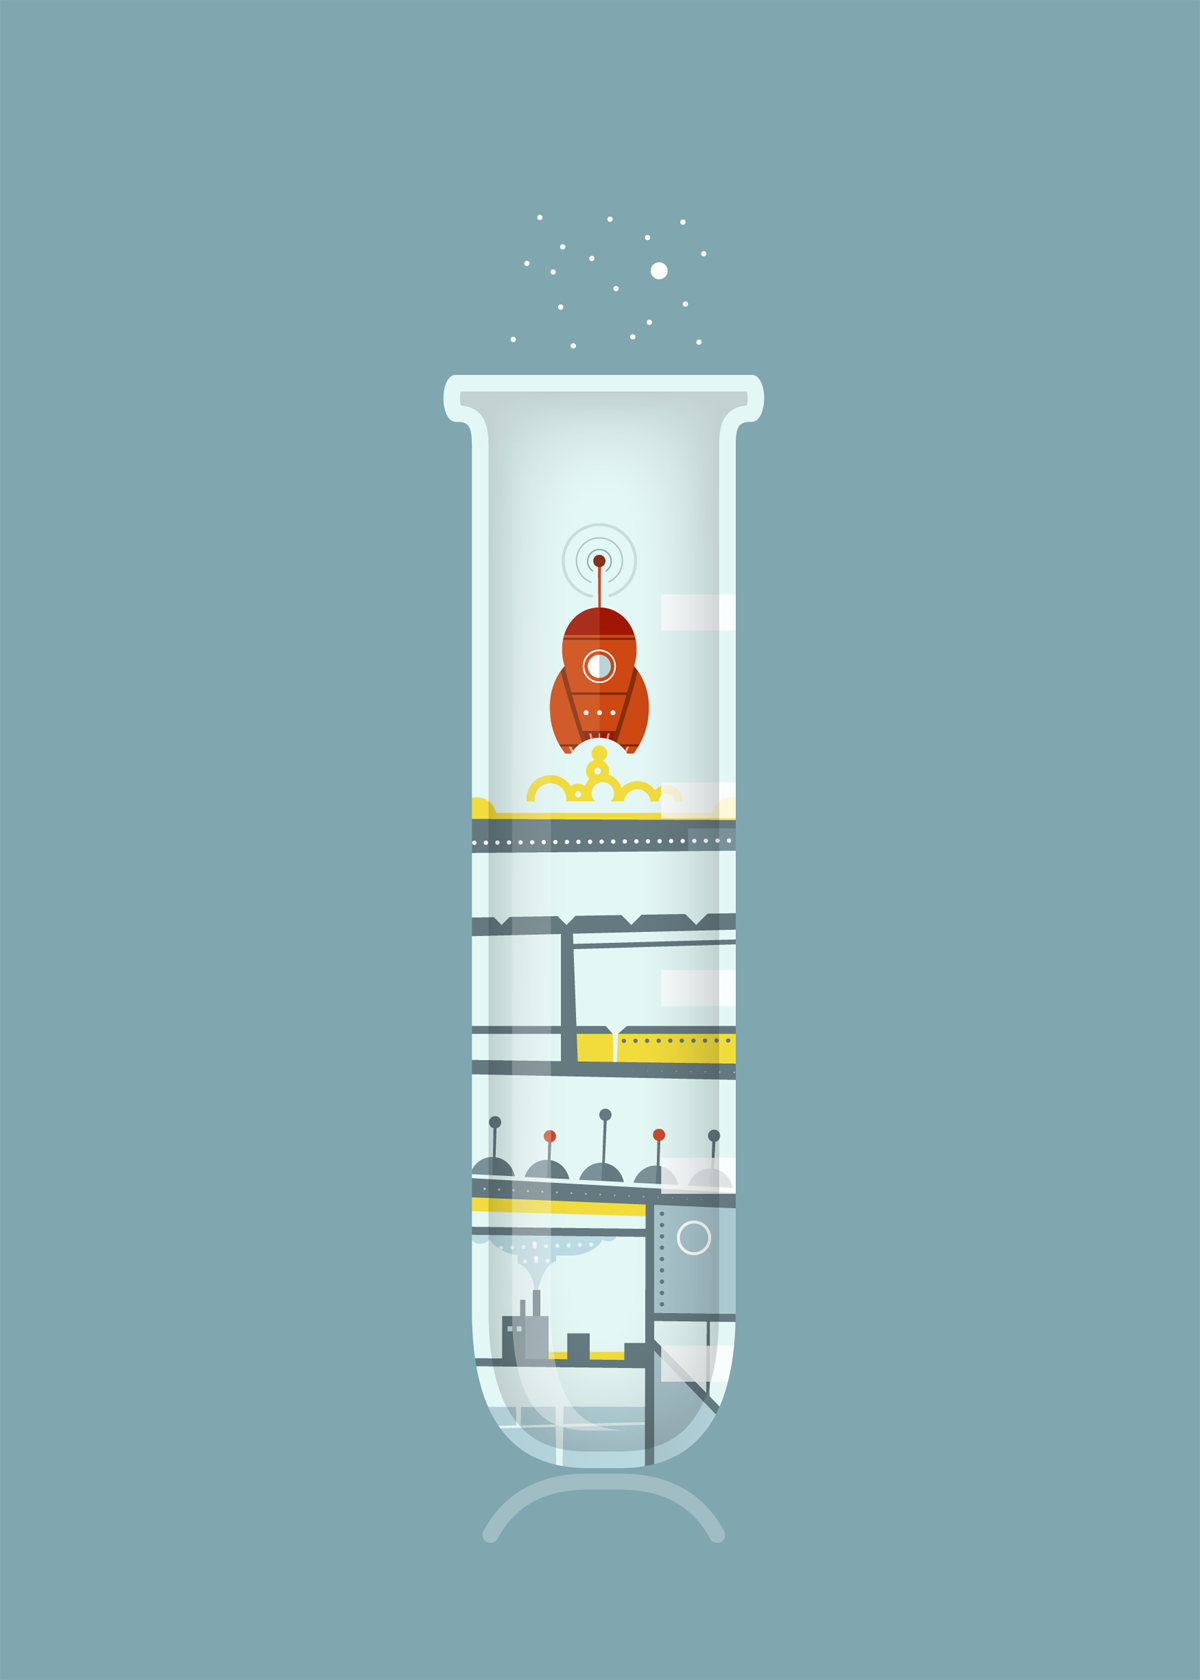
\includegraphics[width=180pt]{endmatter/colophon.png}
\end{figure}

% If you don't want an image in the colophon:
% \vspace*{200pt}

\begin{center}
\parbox{200pt}{\lettrine[lines=3,slope=-2pt,nindent=-4pt]{\textcolor{SchoolColor}{T}}{his thesis was typeset} using \LaTeX, originally developed by Leslie Lamport and based on Donald Knuth's \TeX. The body text is set in 11 point Egenolff-Berner Garamond, a revival of Claude Garamont's humanist typeface. The above illustration, ``Science Experiment 02'', was created by Ben Schlitter and released under \href{http://creativecommons.org/licenses/by-nc-nd/3.0/}{\textsc{cc by-nc-nd 3.0}}. The cover was designed by the amazing Helena Rasche and myself.

\ \\
Hint for the puzzles on the back cover: esoteric programming languages. }
\end{center}


\end{document}
